\documentclass[12pt]{report}

\usepackage{urcsthesis}
%\usepackage{urcsbiblio}

\usepackage[square]{natbib}

\usepackage{amsmath}
\usepackage{amssymb}
\usepackage{amsthm}
\usepackage{graphicx}
\usepackage{subfigure}
\usepackage{boxedminipage}
%\usepackage{cite}
\usepackage{balance}
\pagestyle{plain}
\usepackage{comment}
\usepackage{algorithmic}
\usepackage{algorithm}
\usepackage{hyperref}

\widowpenalty10000
\clubpenalty10000

\begin{document}

\title{A Higher Order Theory of Locality and Its Application in
  Multicore Cache Management}
\author{Xiaoya Xiang}
\thesissupervisor{Chen Ding}

\maketitle

\newtheorem{theorem}{\sc \bf Theorem}[section]
\newtheorem{lemma}[theorem]{\sc \bf Lemma}
\newtheorem{fact}[theorem]{\sc \bf Fact}
\newtheorem{corollary}[theorem]{\sc Corollary}
\newtheorem{definition}[theorem]{\sc Definition}


% no long needed after including amsthm package
%
\begin{comment}
\newenvironment{proof}[1][\sc \bf Proof]{\begin{trivlist}
\item[\hskip \labelsep {\bfseries #1}]}{\end{trivlist}}
\newenvironment{definition}[1][\sc \bf Definition]{\begin{trivlist}
\item[\hskip \labelsep {\bfseries #1}]}{\end{trivlist}}
\newenvironment{example}[1][\sc \bf Example]{\begin{trivlist}
\item[\hskip \labelsep {\bfseries #1}]}{\end{trivlist}}
\newenvironment{remark}[1][\sc \bf Remark]{\begin{trivlist}
\item[\hskip \labelsep {\bfseries #1}]}{\end{trivlist}}

\newcommand{\qed}{\nobreak \ifvmode \relax \else
      \ifdim\lastskip<1.5em \hskip-\lastskip
      \hskip1.5em plus0em minus0.5em \fi \nobreak
      \vrule height0.75em width0.5em depth0.25em\fi}
\end{comment}


\begin{curriculumvitae}
The author was born in Jingmen, Hubei, China. She graduated in 2005 from
Huazhong University of Science and Technology with a Bachelor of
Science degree in Computer Science and Technology and at the same time from
Wuhan University with a Bachelor of Science degree in Finance. She
continued studying Computer Science at the Institute of Computing
Technology, Chinese Academy of Sciences, and got a Master of Science
degree in 2008. Then she joined the graduate program at the
University of Rochester, focusing on program locality models and
program corun penalty analysis. She was supervised by Professor Chen
Ding during her doctoral study. She interned at IBM Toronto in the
summers of 2009 and 2010 and at Google in the summer of 2011. Her main
research progress was published as below.

\begin{itemize}
\item Xiaoya Xiang, Bin Bao, Tongxin Bai, Chen Ding, and Trishul
  M. Chilimbi, All-window profiling and composable models of cache sharing.
In Proceedings of the 16th ACM SIGPLAN Symposium on Principles and Practice
of Parallel Programming, San Antonio, Texas, USA, 2011, pages 91-102.
\item Xiaoya Xiang, Bin Bao, Chen Ding, and Yaoqing Gao, Linear-time
  modeling of program working set in shared cache. In Proceedings of
  the 20th International Conference on Parallel Architectures and
  Compilation Techniques, Galveston Island, Texas, USA, 2011, pages 350-360.
\item Xiaoya Xiang and Bin Bao, How to Fit Program Footprint
  Curves. In ACM SIGPLAN Workshop on Memory Systems Performance and
  Correctness, San Jose, California, USA, 2011.
\item Xiaoya Xiang, Bin Bao, Chen Ding, and Kai Shen. Cache conscious
  task regrouping on multicore processors. In Proceedings of the 12th
  IEEE/ACM International Symposium on Cluster, Cloud and Grid
  Computing, Ottawa, Canada, 2012, pages 603-611.
\item Xiaoya Xiang, Chen Ding, Hao Luo, and Bin Bao, HOTL: a Higher
  Order Theory of Locality. In Proceedings of the 18th International
  Conference on Architectural Support for Programming Languages and
  Operating Systems, Houston, Texas, USA, 2013.
\end{itemize}

\end{curriculumvitae}

\begin{acknowledgments}
I would like to thank my advisor, Professor Chen Ding, for his
guidance during my doctoral study. From him, I learned not only
research skill but also research attitude. He is intelligent, erudite,
nice, and tolerant. Most important, he is very supportive whenever I
face challenges. There were a couple of times that I felt hopeless
about the research topic I worked on and wanted to give up. Chen worked
closely with me to explore the potential of my work until it was widely 
recognized. Chen also helped me a lot with English writing. 

I appreciate the help from my committee members, Michael Scott, Sandhya
Dwarkadas, and Michael Gage. They did a great job of keeping me on the right
track and widening my knowledge. The high-level suggestions they gave
saved me a lot of time on unnecessary details and repeating other
people's work. I would like to thank Kai Shen and Yaoqing Gao. Kai
gave me a lot of support when we were working on task grouping. Yaoqing was my mentor when I interned at IBM Toronto. The idea
of using average footprint was developed when I worked with Yaoqing. 

Special thanks to my teammates, Tongxin, Xiaoming, Bin, Hao,
and Jake. I learned a lot from the discussions with them, especially
Bin. In addition to theoretical suggestions, Bin also gave me a hand
collecting experiment results.

I am very grateful to my friends in Rochester, especially the ones
in the Computer Science department, Katie (for all the parties celebrating
Chinese Festivals), Kyle and his wife Kristy (for the concerts and
books), Licheng, Hongzhou and his wife Shang, Rongrong, Yi, Xiao and
his wife Yang, Xu, Zhuan, Li and his girlfriend Ran, and Yu. Sorry
that I am not able to list you all because of the limited
space. Thanks for adding more colors to my life in Rochester!
Especially, thanks to Zhuan for teaching me how to drive, and thanks to Yuzhe
for teaching me how to swim. I would also like to thank JoMarie, Marty
and Pat. Thanks for your support in many aspects to make my life
abroad much easier.

Last and most important. I would like to thank my parents, who taught
me how to face the world with love and smile. Thanks to Ximing for pushing
me finish this thesis. 
\end{acknowledgments}

\begin{abstract}
  As multi-core processors become commonplace and cloud computing is
  gaining acceptance, applications are increasingly run in parallel
  over a shared memory hierarchy.  While the traditional machine and
  program metrics such as miss ratio and reuse distance can precisely
  characterize the memory performance of a single program, they are
  not composable and therefore cannot model the dynamic interaction
  between simultaneously running programs.

  This dissertation presents an alternative metric called program
  footprint.  Given a program execution, its footprint is the amount
  of data accessed in a given time period.  The footprint is
  composable --- the aggregate footprint of a set of programs is the
  sum of the footprint of the individual footprints.  The dissertation
  presents the following techniques

  \begin{itemize}
  \item \emph{Near real-time footprint measurement}, first by using two novel
    algorithms, one for footprint distribution and the other footprint
    average, and then by run-time sampling.
  \item \emph{A higher order theory of cache locality}, which shows
    that traditional metrics can be derived from the footprint and
    vice versa.  (As a result, previous locality metrics can also be
    obtained in near real time.)
  \item \emph{Composable model of cache sharing}, by footprint
    composition, which is faster and simpler to use
    than previous reuse-distance based models.
  \item \emph{Cache-conscious task regrouping}, which reorganizes a
    parallel workload to minimize the interference in shared cache.
    \end{itemize}

Through these techniques, the dissertation establishes the thesis that
\emph{program interaction in shared cache can be efficiently and accurately
modeled and dynamically optimized}.

\end{abstract}

\begin{contributors}
This work was supervised by a dissertation committee which consists of
Professor Chen Ding, Michael Scott, and Sandhya Dwarkadas from the
Department of Computer Science, Professor Michael Gage from the
Department of Mathematics. The comparison with the working set theory
was done in collaboration with Professor Peter Denning and Chen
Ding. Professor Chen Ding contributed to the idea of both lifetime
sampling and higher order theory of locality and also contributed many
beautiful sentences to this thesis.  Profiling tools used
throughout the paper was built based on Pin, a dynamic binary
instrumentation tool developed by Intel. Part of the footprint and
reuse distance traces were collected using the parallel collecting
script written by Bin Bao. Bin also helped running the script for some
experiments. The bin-mapping library used for plotting histograms were
provided by Tongxin Bai. All other work covered in the dissertation
was completed by the student independently. The student is supported
by IBM Center for Advanced Studies Fellowships. The research is also
supported by the National Science Foundation (Contract No. CCF-1116104,
CCF-0963759, CNS-0834566). 
\end{contributors}

\tableofcontents

\listoftables

\listoffigures

\chapter{Introduction}
\label{chap:intro}

\section{Problem Statement}

Computing is ubiquitous, in science, engineering, business and
everyday life; and in cloud, desktop, and handheld.  Most of today's
programs run on multicore processors, and as a result they interact and
interfere.  It is important to control the
interaction and reduce the interference, for achieving not just
good performance, but also stable performance in a
dynamic environment; not just for parallel code, but also sequential
applications running in parallel.

Cache sharing is the primary cause of program interference.  Modern
applications spend most of the time accessing memory, and
most memory accesses, over 99\% typically, happen in cache.  On a
commodity system today --- 2 to 8
processors  (sockets), 2 to 6 physical cores per processor, and 2 to 4 hyperthreaded logical cores per physical core --- nearly a hundred programs
can run together in parallel.  

Partitioned cache solves the interference problem by program
isolation. However, cache partitioning is wasteful when only one program is
running and inefficient when co-run programs share data.  Current
multicore processors use a mix of private and shared cache. For
example, Intel Nehalem has 256K L2 cache per core and 4MB to 8MB L3
cache shared by all cores. IBM Power 7 has 8 cores, with 256KB L2
cache per core and 32MB L3 shared by all cores.

Depending on which CPU they are using, programs
interact in different ways.  Physical cores have private
cache at the first and second levels but share the last level cache.
Logical cores share the cache at all levels.  Different processors do
not share cache.  However, they share the memory bandwidth, and the
demand of memory bandwidth depends entirely on the performance of the
cache.  In addition, some caching policies, e.g. inclusive cache on
Intel machines, may induce indirect interaction, where a program may lose data in
its private cache due to the data access by another program in the shared
cache.

% eviction in the shared cache necessitates the eviction in the
% private  cache, 

The advent of cache sharing is reminiscent of the dawn of memory
sharing in early days of computing when time sharing was
invented.  The problem of memory management has been well studied
and solved, and modern operating systems manage memory for a large number of programs as a matter of course.
However, cache is managed by hardware not the operating system.

The problem of cache sharing is more complex.  Cache has multiple
levels and varying mixes of exclusivity and sharing.  Events of cache
accesses and replacements are orders of magnitude more frequent than memory
access and paging.  A single program may access cache a billion times
a second and can wipe out the entire content of the cache in less than
a millisecond.  The intensity multiplies when more programs are run
in parallel.  Furthermore, the size of cache is fixed on a given machine.
One cannot get online and buy more cache as one can with memory.

Cache interference is asymmetrical, non-linear, and circular.  The
asymmetry was shown in early experiments by \cite{Zhang+:EuroSys09} at
Rochester and confirmed by later studies.
In a pair-run experiment we conducted using Zhang's setup, one program
becomes 85\% slower, while its partner is only 15\% slower.  The
interference changes from program to program.  The effect depends not
as much on how many programs are running as on which programs are
running.  Finally, the interference has self feedback because the behavior of
one program affects the peer programs which affect itself.

\section{All-window Footprint}

Locality is a basic property of a computing system.  \cite{Denning:TSE80}
defined locality as ``a concept that a program favors a subset of its
segments during extended intervals (phases).'' 
There is a difference between the data that a program has
and the data that the program is actively using.  The latter is a
subset of the former.  \cite{Denning:CACM68} coined the widely used term \emph{the working set}
to refer to the active data subset.

The performance depends on how fast a computer system
provides access to the active data subset.  The access time of 
the other data is irrelevant.  
Locality analysis, as it
quantifies the active data usage, is naturally a pre-requisite to
memory system design, for the oft quoted reason``we cannot improve
what we cannot measure.''

This dissertation measures the active data usage by a concept we call
the \emph{footprint}.  A footprint is the amount of data accessed in a
time window.  It is the size of the active data.  

As an illustration, let's use the
word ``footprint'' as a short trace and treat its 9 occurrences of 7 letters
as 9 accesses to 7 data blocks.  Every sub-string is a time window in the trace.  Its footprint is the number of
distinct letters in the sub-string.  

\begin{figure}[h]
\centering
\includegraphics[width=14cm]{figures/intro/footprintfp}
\caption{The footprint of 36 windows in the contrived 9-element trace ``footprint''}
\label{fig:fpfp}
\end{figure}

There are 45 windows in the 9-element trace (9 choose 2 plus 9).  The 45 footprints are
plotted in Figure~\ref{fig:fpfp}.  As the window size (x-axis) increases from
1 to 9, and the footprint (y-axis) grows from 1 to 7.  Take for example the extreme cases.  The shortest
windows have a unit length.  There are 9 such windows, and their
footprint is obviously 1.  The longest
window is the whole trace, and the footprint is 7.  

It is natural that a longer period of execution accesses 
a greater amount of data.  The footprint quantifies the relation by showing the size of active data in all periods of
execution, as shown in the plot in Figure~\ref{fig:fpfp} for
the example trace.  

In practice, the footprint is too numerous to enumerate.  The
number of time windows is quadratic to the length of the
trace.\footnote{If the trace length is $n$, the number of windows (and
  hence footprints) is ${{n}\choose{2}} + n = \frac{n*(n+1)}{2}$ or $O(n^2)$ asymptotically.}
Assuming a program running for 10
seconds on a 3GHz processor, we have $3E10$ CPU cycles in
the execution and $4.5E20$
distinct windows.  

\begin{figure}[]
  \centering
  \includegraphics[width=11cm,height=8cm]{figures/intro/WindowSizes2}
  \caption{The scale of the problem shown by the number of footprint
    windows in a program execution, compared to the size of a galaxy and the universe.  Reproduced from \cite{Brock+:BDAW13}.}
  \label{fig:bigdata}
\end{figure}

\cite{Brock+:BDAW13} described program analysis as a Big Data problem, 
and showed the scale of the problem by the number of time
windows in an execution.
Figure~\ref{fig:bigdata} shows that as the length of execution increases from 1
second to 1 month, the number of CPU cycles ($n$) ranges from $3E9$ to
$2E15$, and the number of distinct execution windows $n \choose 2$
from $4.5E18$ to $5.8E29$, that is, from 4 sextillion to over a half
nonillion.  

As a dynamic analysis problem, the scale 
quickly reaches the size of any static problem.  As a comparison, 
the figure shows the radius of the Milky Way in centimeters, 48 sextillion,
and the radius of the observable universe, 44 octillion.

The purpose of a footprint theory is to overcome the enormity of the
analysis problem, characterize the active data usage in all windows
and make it useful for system analysis and optimization.

\begin{comment}
``footprint''

% Ruby script for generating (x,y) coordinates for the footprint plot

afp = {}
afp[1] = [1,1,1,1,1,1,1,1,1]
afp[2] = [2,1,2,2,2,2,2,2]
afp[3] = [2,2,3,3,3,3,3]
afp[4] = [3,3,4,4,4,4]
afp[5] = [4,4,5,5,5]
afp[6] = [5,5,6,6]
afp[7] = [6,6,6]
afp[8] = [7,7]
afp[9] = [7]

# frequency count
freqs = Hash.new{ 0 }

def perturb( wfp, freqs, delta = 0.05 ) 
  freq = freqs[wfp]
  freqs[wfp] = freq + 1
  wfp.collect{ |i| i + freq*delta }
end

xs, ys = [], []
afp.each do |ws, fps|
  fps.each do |fp| 
     x, y = perturb([ws,fp], freqs)
     xs << x.to_s
     ys << y.to_s
  end
end
puts "x = c( #{xs * ', '} )\ny = c( #{ys * ', '} )"

% R script for plotting, pch=3 is +, 4 is cross, see http://sphaerula.com/legacy/R/plotSymbols.html

dev.new(width=6, height=4)
plot( x, y, pch=3, cex=2, col="blue", xlab = "window size", ylab = "footprint", main = "all-window 'footprint' footprint" )
axis(1, seq(9), seq(9))
dev.copy2pdf(file="footprintfp.pdf")
dev.off()

\end{comment}

\section{A New Locality Theory}
\label{sec:intro:theory}

For locality analysis, the basic unit of information is a data access,
and the basic relation is a data reuse.  The theory of locality is
concerned with the fundamental properties of data accesses and reuses,
just as the graph theory is with nodes and their links.

The core of the dissertation is a new locality theory consisting of a
set of formal definitions, algorithms and properties based on the
concept of the footprint.  This section introduces the four components of the theory and their supporting techniques.

\paragraph{Footprint Measurement}
The enormous scale of all-window analysis is tackled by a series of
three algorithms.  Each is two orders of magnitude more efficient than
the previous one.

\begin{itemize}
\item \emph{Footprint distribution analysis}, which enumerates 
  all $O(n^2)$ footprints in $O(n \log m)$ time, where $n$ is the 
  length of the trace and $m$ the maximal footprint.
\item \emph{Average footprint analysis}, which reduces the cost to
  linear time $O(n)$ by computing the average without enumerating all
  footprints.
\item \emph{Footprint sampling}, which samples limited-size windows and reduces the cost to sub-linear.
\end{itemize}

The distribution analysis is the first algorithm to measure
all-window footprint.  As it actually enumerates all footprints, it
finds the largest, smallest, median, average, and any percentile
footprint for each window length.  However, the cost is sometimes
thousands of times slowdown.

The second algorithm computes just the average footprint, and the
cost is reduced from a thousand times slowdown to about 20 times.  Being a linear time
algorithm, it is scalable in that the cost increases proportionally to
the length of the program execution.

The cache on a real machine has a finite size, so an analysis does
not have to consider windows whose footprint is greater than the cache
size.  In addition, the behavior of a long running
program tends to repeat itself.  Furthermore, on modern
processors, the analysis can be carried out on a separate core in
parallel with the analyzed execution.
Footprint sampling specializes and parallelizes the
analysis for a specific machine and program.  The average
cost is reduced to 0.5\% of the running time of the unmodified execution.

The algorithmic development attains immense gains in both
computational complexity and implementation efficiency.  As the baseline, the first algorithm is
already a breakthrough since there was no previous viable solution for
all-window analysis.  The second and the third algorithm each
improves efficiency by another
orders of magnitude, eventually making it fast enough for
real-time analysis.  This has a beneficial impact elsewhere, because
the footprint can be used to compute other locality
metrics, as we will see in the next part of the footprint theory.

\paragraph{Composability}
As a locality metric, footprint is unique because it is composable.  
Let the average footprint of a program be $prog.fp(x)$ for window
length $x$.  If we have $k$ programs $prog_1, prog_2, \dots,
prog_k$ actively sharing the cache, the aggregate footprint is
the sum of the individual footprints.

$$ corun.fp(x) = \sum_{i=1}^k prog_i.fp(x) $$

In comparison, the miss ratio is not composable.  Consider two
programs sharing the cache.  The co-run miss ratio will change
compared to the solo-run miss ratio since each program has
now a fraction instead of the whole cache.  The change in miss ratio, as mentioned
earlier, is asymmetrical, non-linear and affected by circular
feedback.  As a result, we cannot directly add the solo-run miss ratio 
to compute the co-run miss
ratio, as we can with the footprint. 

Another locality metric is reuse distance.  Reuse distance does
not depend on cache parameters but as we will explain
in Section~\ref{sec:back:rd}, it is also not composable.

% two bodies of water can be composed into a bigger body but two bags
% cannot be composed into a bigger bag.

As mentioned earlier, we can measure the average as well as
the distribution of footprints.  
The average footprint is immediately composable.  The distribution, although composable, requires
a convolution which is expensive to compute and difficult
to visualize.  In this thesis except in Section~\ref{sec:all-fp}, 
the term footprint when unqualified means the average
footprint.

The next question is whether the composability from the footprint 
can help in analyzing the miss ratio and other locality metrics in
shared cache.  This is solved in
the third part of the new theory.

\paragraph{Locality Metrics Conversion}
The footprint is convertible with a number of other metrics,
as we will show in Chapter~\ref{chap:model}.  For example, let $mr(c)$ be the miss ratio
for cache size $c$.  The conversion formula we will derive is the
following:

$$\textit{mr}(c) = \frac{\textit{fp}(x+\Delta x) - fp(x)}{\Delta x}$$

\noindent where $c = \textit{fp}(x)$.  If these are continuous
functions, we would say that the miss ratio is the derivative function
of the footprint.  

The higher order mathematics implies stricter
properties.  The derived metric, the miss ratio, should be
non-decreasing.  For this to hold in all cases, the source function 
must be not just non-decreasing but also
concave.  We will prove that the average
footprint has this stronger property.  

The conversion is reversible.  If we have the miss ratios of all cache
sizes, we can reverse the formula and compute the average
footprint.  The reverse process is the analogous of integration for
a discrete function.  

% Let the inter-miss time for cache size $k$ be $im(k) =
% \frac{1}{mr(k)}$, the reciprocal of the miss rate.  The window length
% of footprint of size $c$

Combining footprint composition and metrics conversion, we can see immediately that if 
we treat co-run programs as one composite task, the
co-run miss ratio can be computed from the aggregate footprint.
Figure~\ref{fig:conversion} shows the derivation by adding
the individual footprints and then converting the sum to the miss ratio.  

\begin{figure}[h]
\centering
\includegraphics[width=10cm]{figures/intro/conversion}
\caption{The joint use of two theoretical properties: composition (dotted line) and conversion (solid lines)}.
\label{fig:conversion}
\end{figure}

Since the conversion formula is reversible, we can switch 
between the footprint and the miss ratio and compose the latter indirectly through the former.  
First, we compute the individual
footprint from the individual miss ratios (of all cache sizes).  Then 
we 
add the individual footprints and finally compute the co-run miss
ratio in the shared cache (of all sizes).  Figure~\ref{fig:conversion}
shows this type of deduction and others that are made possible by
composition and conversion.  In particular, the figure shows how to compose another locality
metric, the reuse distance.  We use the terms private reuse distance (PRD)
and concurrent reuse distance (CRD), as introduced by \cite{WuY:PACT11,Wu+:ISCA13}.

The solution of composition raises the problem of decomposition.
The co-run miss ratio does not tell us the contribution from each
program.  To see the individual effects, we need more elaborate models.

\paragraph{Composable Locality Models}
We say a model is composable if the co-run result can be computed from
solo-run results, not just for the co-run group as a whole but also
for the co-run effect on each individual program.  In other words,
a composable model must be both composable and decomposable.

First, let's summarize the three reasons that footprint-based models
are general and efficient for composition.  The footprint is

\begin{itemize}
\item \emph{Machine independent.}  The analysis is based on data
  accesses, not cache misses.  It takes a single pass to analyze a
  trace for all cache sizes, and the result is not affected by program
  instrumentation.  In comparison, it is inescapable for direct measurement to be
  affected by instrumentation.
\item \emph{Clean-room statistics.}  The
  footprint of one program can be measured in a co-run environment, unperturbed by
  other programs.  The clean-room effect solves the chicken-or-egg
  problem of direct measurement: the behavior of one program depends on 
  its peer, but the peer behavior in turn depends on itself.
\item \emph{Peer independent.}  Locality metrics are
  defined on and for a program itself, independent of co-run peers.
  The analysis of cache sharing does not require actual cache 
  sharing.  The co-run effect is computed rather than measured.
\item \emph{Static composition.}  There are $2^P$ co-run combinations
  for $P$ programs.  The footprint model can predict the interference
  in these $2^P$ runs by testing $P$ single-program runs.  For the $P$
  sequential runs, one can choose to run them one by one or some of
  them in parallel to increase speed. The composition is static if
  there is no actual co-run; otherwise we say the composition is
  dynamic.  Here dynamic composition means parallel testing.  Static
  composition does not need parallel testing at all.
\end{itemize}

To compute the co-run effect on each individual program, the
dissertation describes three models.  The models solve the decomposition
problem as a composition problem: how one program is affected
by its peers.

% formalism must work out so the sum of the predicted individual
% effects gives the same result as the predicted overall effect.

\begin{itemize}
\item \emph{Composition by reuse distance and footprint} 
Variations of this model were invented by
  \cite{ThiebautS:TOCS87} and \cite{Suh+:ICS01} for time-sharing systems (time-switched cache sharing) and \cite{Chandra+:HPCA05} for multicore (continuous cache sharing).  With fast
  footprint measurement, we will show that the cost of the model is limited by the time
  required for reuse distance measurement.
\item \emph{Composition by footprint only} The second model converts the
  footprint into reuse distance, so it no longer needs to measure 
the reuse distance and can be
  hundreds of times faster.
\item \emph{Composition by program pressure and sensitivity} The last
  model is as fast as the second model but more intuitive and easier
  to use.  It characterizes the behavior of a program
  by two factors, pressure and sensitivity.  The two can be
  visualized as two curves.  Performance composition is as simple as
  looking up related values on the two curves.
\end{itemize}

Using the composable models, the thesis will answer a number of
long-standing questions about shared cache, including:

\begin{itemize}
\item Is there a machine independent way to compare programs by their
  shared cache behavior?  How do programs differ within and
  between application domains?
\item How does the interference correlate with the miss ratio?  If a
  program has a higher miss ratio, does it always exert a higher interference?
\item Can the shared cache be viewed as a confederation of per-program
  partitions?  In the shared cache, the division of space is dynamic and
  demand driven.  Does the dynamism provides an inherent advantage
  for cache sharing over cache partitioning?
\end{itemize}

These models are theoretical.  They are appealing due to the
generality.  The footprint is defined on a program trace without
knowing co-run peers or machine parameters (other than having shared
cache).  There are many sources of error due to the fact that the
basic models do not consider the effect of cache associativity,
program phase behavior, the time dilation due to interference, the
filtering effect in a multi-level cache hierarchy, and the impact of
the prefetcher.  A theory must be validated to be practically
relevant.  The thesis will show evaluate these model on real systems
and compare theoretical predictions with actual miss counts measured
by hardware counters.  It will also show extensions of the models to
consider time dilation, cache associativity, and program phases.
 
By developing and validating the new theory, this thesis will
quantify the essential aspects of program behavior in shared cache and
as a result enhance our ability to understand and manage program
interaction on multicore systems.


\section{Thesis Statement and Organization}

{\bf Thesis statement}  
\emph{The interaction of computer programs in shared cache can be
efficiently and accurately modeled and dynamically optimized using 
a footprint theory of locality that includes footprint measurement,
conversion, and composable modeling.}

The technical content is organized in five chapters as follows. 

\begin{itemize}
\item Chapter~\ref{chap:background} gives the background of locality
theories and techniques, including locality metrics and measurements
and previous cache sharing models. 

\item Chapter~\ref{chap:fp} presents the three algorithms for
  footprint measurement.  The first measures the footprint
  distribution, the second the average footprint.  The first two
  algorithms are precise and asymptotically efficient.  The third
  algorithm improves the practical efficiency through footprint
  sampling.

\item Chapter~\ref{chap:model} presents a higher order theory for the
  mutual conversion between five locality metrics.  It shows
  the correctness condition for the conversions.  Theoretically, it extends
  the work-set theory and confirms Denning's Law of Locality.
  Empirically, it enables near real-time locality analysis.

\item Chapter~\ref{chap:corun} describes the pressure-sensitivity
  model where the behavior of a program in shared cache is completely
  characterized by just two factors.  The model is built from the new
  theory, the calculation (of miss ratios) extremely simple, and the
  result consistently accurate.

\item Chapter~\ref{chap:regroup} presents a cache-conscious task
  regrouping framework, which uses the new models to minimize cache
  interference on multicore processors. 
\end{itemize}

The style of the work is mixed, so is the presentation: formal and
algorithmic for footprint measurement, mathematical for metrics
conversion, and experimental and scientific for performance
calibration and validation.


\chapter{Background on Metrics, Models and Management}
\label{chap:background}

Fast development of multi-core processing brings resource usage into a
cloudy world.  Performance metrics and models are prerequisites for
scientific understanding and optimization.  This chapter introduces
the area of locality analysis and optimization and reviews the
research work leading to this thesis.  It divides the material into
metrics and their measurement, metrics conversion, locality and
performance models of shared cache, and other related techniques.

% While task co-locating and cloud computing explore the potential
% synergy of resource utilization, there are many ways the performance
% is compromised due to conflicts. Either cache sharing or partitioning
% may cause performance problems.

\section{Core Metrics and Measurement}
\label{sec:bg-locality}

Locality was started as an observation that programs do not use all
their data at all times~\citep{Denning:TSE80}.  After decades of
research, it has developed into an important scientific field.  At its
foundation are locality metrics, so the concept and its effect can be
measured.  Among the basic problems are the measurement speed and
accuracy of these metrics.

\subsection{Miss Ratio and Execution Time} 
The performance of a single or a group of programs can be
observed directly.  The hardware performance counters on modern
machines enable a tool to measure program speed and count cache misses
in real-time with little costs.  However, direct observation
has difficulties in characterizing the locality cleanly due to 
dependences to the observation environment.

\begin{itemize}
\item \emph{Machine dependence.}  Different machines have different
  memory hierarchies and processors, so we cannot compare the locality
  in different programs entirely based on their performance.
\item \emph{Instrumentation dependence.}  The analysis code itself consumes
  processor and cache resources.  It may not be
  possible to completely separate the effect of the instrumentation.
\item \emph{Peer dependence.}  It is unknown how the performance
  has changed due to cache sharing.  It would have required another
  test on an unloaded system.  It is also unknown how the
  performance will change if the peer programs change.
\end{itemize}

The effect of cache on performance is often disruptive.  
Chilimbi once compared the phenomenon to ``strolling until suddenly falling over a
cliff.''\footnote{Trishul Chilimbi made this analogy in a
  presentation in 2002~\citep{ChilimbiH:PLDI02}.}  The danger is
greater in a shared environment.  As more programs are added, the
combined working set grows.  When it exceeds the size of the shared
cache, sharp performance drops would ensue.  Being peer and machine
dependent, direct testing cannot foresee a pending calamity.  Worse,
it cannot even tell whether a given parallel mix is efficient or not
without testing them individually first.

\subsection{Reuse Distance}
\label{sec:back:rd}

Instead of direct observation, off-line trace profiling can be more thorough and
can not just evaluate but also optimize a program.  % identifying causes
The most commonly used
metric is the reuse distance.  For each memory access in a
single-task execution, the reuse distance (i.e. LRU stack
distance defined by \citet{Mattson+:IBM70}) is the number of distinct data
elements accessed between this and the previous access to the same
data.  \citep{JiangZ:SIGMetrics02} also called it the inter-reference recency
(IRR).  

The reuse distance quantifies the locality of every memory access.
The locality of a program, or a loop and function inside it, is the
collection of all its reuse distances.  The collective result can be
represented as a distribution.  It is called a \emph{locality
  signature} by \citep{Zhong+:TOPLAS09} and \emph{locality profile} by
\citep{Wu+:ISCA13}.  It can be viewed as a discrete probability
density function, showing the probability of a memory access having a
certain locality.

\subsubsection{Relation with Cache Performance}

In the absence of cache sharing, the capacity miss ratio can be
written as the fraction of the reuse distance that exceeds the cache
size~\citep{Mattson+:IBM70}.  Let the test program be $A$ and cache
size be $C$, we have

\begin{equation*}
\begin{array}{l}
  P(\mbox{capacity miss by A})  = P(\mbox{A's reuse distance $>C$})
\end{array}
\end{equation*}

The reuse distance is machine independent but can give the capacity
miss ratio for cache of all sizes, as the formula shows.  More
elaborate models have been developed to estimate the miss ratio in not
just fully-associative but also direct mapped and set-associative
cache~\citep{Smith:ICSE76,HillS:TOC89,MarinM:SIGMETRICS04}.

% and for not just the tested but also all inputs of a
% program~\citep{Zhong+:TOPLAS09,Zhong+:TOC07,MarinM:SIGMETRICS04}.

\subsubsection{Miss Ratio Curve (MRC)}

The miss ratio curve (MRC) shows the miss ratio of all its cache sizes
as a discrete function.  It is easy to visualize and shows directly
the trade-off between performance and cache size.  For fully
associative LRU cache, the miss ratio curve is equivalent to the reuse
distance distribution, as the preceding formula shows.  The problem is
equivalent in theory whether it is measuring the miss ratio curve or
the reuse distance.  In practice, the miss ratio curve is defined for
only practical cache sizes, i.e. powers of two between some range,
e.g. 32KB and 8MB.  The reuse distance has the full range between 1
and the size of program data.

The full range of reuse distance represents the complete temporal
locality.  The miss ratio curve is a projection of the full
information on a subset of cache sizes.  The two would be equivalent if the
miss ratio is defined for all cache sizes between 1 and infinity.  The
unbounded size of the representation is consistent with the
theoretical result of \citet{SnirY:locality05}, who showed that
we cannot represent the temporal locality with just one or a few
numbers.  There are other metrics that represent similar information.
Chapter~\ref{chap:model} will discuss formal properties and place the
reuse distance and the miss ratio curve in relation with other
locality metrics.  In this section, we review prior work on the
measurement of the reuse distance and the miss ratio curve
together.

\subsubsection{Locality Characterization and Optimization}

% Reuse distance has found many uses in workload characterization
% and program optimization. 

Reuse distance has found many uses in workload characterization
and program optimization. The signature shows quantitatively how the
locality changes with the program input, and
the changes can be predicted as in whole-program locality analysis
\citep{Zhong+:TOPLAS09,MarinM:SIGMETRICS04,Fang+:CC06}, which is used to predict the miss ratio of all
inputs and cache sizes\citep{Zhong+:TOC07}.  The signature can be
also modeled for each memory reference and used to find critical
memory loads and important program paths, as shown by Fang et
al.~[\citeyear{Fang+:PACT05,Fang+:CC06}] \citet{MarinM:SIGMETRICS04}
models the locality signature at reference, loop, and function levels
to predict performance across different computer architectures.
Beyls and D'Hollande [\citeyear{BeylsD:HPCC06,BeylsD:CF06}] builds a
program tuning tool \emph{SLO}, which identifies the cause of long
distance reuses and gives improvement suggestions for restructuring the
code.  In addition to cache misses, reuse distance has been used to predict
cross-architecture performance (profiling on one machine and
predicting for another) \citep{MarinM:SIGMETRICS04},
response time in server systems~\citep{Kelly+:HP04}, and
usage patterns in web reference streams~\citep{Almeida+:PDIS96}. 
\citet{Zhong+:TOPLAS09} classifies these and other uses of reuse
distance as ``Five Dimensions of Locality'' and reviews the analysis
techniques for program input, code, data, execution phase and program
interaction.  

\bigskip

Reuse distance provides a common foundation to model behavior, predict
machine performance, and guide program optimization. 
Locality analysis is to summarize and decompose reuse distances.
Locality optimization is to shorten long reuse
distances.  In addition, it is free of the machine, instrumentation
and peer dependences.  The downside, however, is the complexity
of measuring reuse distance.  Next we review the existing work on
the measurement problem.

\subsubsection{Precise Measurement}
Reuse distance is one of the stack distances defined in the seminal
paper in 1970 by \citet{Mattson+:IBM70}. The stack
algorithm in the paper needed $O(nm)$ to profile a trace with $n$ accesses to $m$
distinct data.  The efficiency has been steadily improved over the
past four decades.  In 1975, \citet{BennettK:IBM75} organized
the trace as a tree and reduced the cost to $O(n \log
n)$.  In 1980, \citet{Olken:LBL81} made the
tree compact and reduced the cost further to $O(n\log m)$.  Till
today, the Olken algorithm is the most efficient asymptotic solution
for precise measurement.

There are practical improvements to the basic algorithms.  {\em Cheetah}
implemented the Olken algorithm using a
splay-tree~\citep{Sugumar:Dissertation}.  It became part of the
widely used SimpleScalar simulator~\citep{BurgerA:TR97}.
\citet{Almasi+:MSP02} used a different tree representation to further
improve the efficiency.
 
Ding and Zhong gave an approximation algorithm, first published in
2003~\citep{DingZ:PLDI03,Zhong+:TOPLAS09}.  It guarantees a relative
precision, e.g. 99\%, and takes $O( n \log \log m)$, which is
effectively linear to $n$ for any practical values of data size $m$.
Zhong et al. also gave an algorithm that guarantees a constant error
bound and does not reduce the asymptotic cost~\citep{Zhong+:LCR02}.
In an independent implementation, \citet{Schuff+:PACT10} reported that the average cost of the
$O(n \log \log m)$ method is as high as
several thousand times slowdown.

Zhong et al. gave a lower bound result showing that the space
cost of precise measurement is at least $O(n \log n)$, indicating that
reuse distance is fundamentally a harder problem than streaming, i.e. 
counting the number of 1's in a sliding window, which can be done
using $O(n)$ space~\citep{Zhong+:TOPLAS09}.  

Cache locality depends on cache management.  Reuse distance shows the
locality in the LRU cache.  For random
replacement cache, \citet{Zhou:NPC10} developed a one-pass
deterministic profiling algorithm to compute the average miss rate
(instead of simulating many times and taking the average).

% This thesis can parallelize the analysis.

\subsubsection{Approximation by Reuse Time}
While the reuse distance counts the number of distinct memory
accesses, the reuse time counts all accesses.  It is simply the difference in logical
time between the previous access and the current reuse and can be measured
quickly in $O(n)$ time.  The 
working set theory used the reuse time (inter-reference gap) to compute the time-window miss
rate~\citep{DenningS:CACM72}.  If we take time-window miss rate as an approximation of the LRU miss
rate, we may say that the working set theory is the first
approximation technique.  

Two series of more recent studies have used the reuse time
to compute the reuse distance.  The first is StatCache and StatStack
by Hagersten and his
students~\citep{BergH:ISPASS04,BergH:SIGMETRICS05,EklovH:ISPASS10,Eklov+:HiPEAC11},\footnote{Berg and
  Hagersten used the term reuse distance for what we mean by reuse
  time~\citep{BergH:ISPASS04}.}
and the second is time-based locality approximation by Shen et
al.~\citep{Shen+:POPL07,ShenS:LCPC08,Jiang+:CC10} 
While the former 
computes the average miss
rate over time range (assuming that the miss probability function does
not change over time), 
the latter calculates the reuse signature to
infer the miss rate.  Although both using statistical analysis,
the precise formulation is different.

In \citet{BergH:ISPASS04},
each access is represented by a random
variable $X_i$, which is assigned 1 if the access $i$ is a miss and 0
otherwise.  Let accesses $i,j$ be two consecutive accesses to some
data.  The reuse time is $j-i$.  Let $P(k)$ be the probability that a
cache block is replaced after $k$ misses.  The following equation
holds

$$E[X_j] = P(X_{i+1}+X_{i+2}+...+X_{j-1})$$

By solving the equation, the goal is to infer the number of cache
misses in every time window.  The problem is actually one of
all-window analysis.  The equation, however, has just $O(n)$
variables.  To produce an estimate, Berg and Hagersten assumed
constant miss rate over time and random cache replacement,\footnote{Zhou studied random cache replacement policy and gave a
one-pass deterministic trace-analysis algorithm to compute the average
miss rate (instead of simulating many times and taking the
average)~\citep{Zhou:NPC10}.} first for
private cache~\citep{BergH:ISPASS04,BergH:SIGMETRICS05} and then for
shared cache~\citep{EklovH:ISPASS10,Eklov+:HiPEAC11}.  

In \citet{Shen+:POPL07}, the key measure is the \emph{interval access
probability} $p(\Delta)$, which is the probability of a randomly chosen
datum $v$ being accessed during a time interval $\Delta$.  It
is computed from the reuse time signature $p_{{}_T}$.

\begin{equation*}
p(\Delta) = \sum_{\tau=1}^\Delta \sum_{\delta=\tau+1}^T
{1\over{N-1}}p_{{}_T}(\delta)
\label{eq:pDelta}
\end{equation*}

\noindent In the derivation, Shen et al. assumed a Bernulli process and LRU
cache replacement, first for sequential
code~\citep{Shen+:POPL07,ShenS:LCPC08} and then for multi-threaded
code~\citep{Jiang+:CC10,Jiang+:HiPEAC10}.  

To model graph algorithms, \citet{Yuan+:ICPP12} defined the notion
\emph{vertex distance} and used statistical analysis to derive the
reuse distance.  The study examines random graphs and scale-free
graphs.  It shows the dual benefits of domain-specific analysis.  On
the one hand, the structure of a graph facilitates locality analysis.
On the other hand, locality analysis reveals the relation between the
properties of a graph, e.g.  edge density, and the efficiency of its
computation.

% These methods have been evaluated experimentally for accuracy (and
% shown effective for miss rate prediction) but in theory do not
% guaranteed to be correct or have a bounded error.

By solving the all-window analysis problem, this thesis provides a
third solution.  In Chapter~\ref{chap:fp}, we will show how to
compute the average footprint using the reuse time.  In
Chapter~\ref{chap:model}, we will how to compute the reuse distance
from the footprint.  Taking together, the two steps give a new
solution of time-based approximation.  Like previous methods, the new
solution is not guaranteed correct.  However, Chapter~\ref{chap:model}
will formalize the condition under which the approximation is correct.

\subsubsection{Sampling Analysis}
Sampling is usually effective to reduce the cost of profiling.  By
choosing a low sampling rate, it may reduce the amount of profiling
work by factors in hundreds or thousands.  
In program analysis, bursty
tracing is widely used, where the execution alternates between short
sampling periods and long hibernation
periods~\citep{ArnoldR:PLDI01,HirzelC:FDDO01,ChilimbiH:PLDI02}.  During
hibernation, the execution happens in the original code and has no
analysis overhead.

Locality sampling, however, is tricker.  Locality is about the time of
data reuse, but the time is unknown until the access actually happens.
The uncertainty has two consequences.  First, the length of the
sampling period cannot be bounded if it is to cover a sampled data
reuse pair.  Second, the analyzer has to keep examining every data
access.  Complete hibernation is effectively impossible.

The problem of locality sampling is addressed by a series of studies, including the
publicly available SLO tool~\citep{BeylsD:HPCC06}, continuous program
optimization~\citep{Cascaval+:PACT05}, bursty reuse distance
sampling~\citep{ZhongC:ISMM08}, and multicore reuse distance
analysis~\citep{Schuff+:PACT10}.
Sampling can drastically reduce the cost if sampled windows 
accurately reflect the behavior of other
windows~\citep{BergH:SIGMETRICS05,EklovH:ISPASS10,Eklov+:HiPEAC11}. 

SLO is developed by \citet{BeylsD:HPCC06}.
It instruments a program to skip every $k$ accesses and take the next
address as a sample.  A bounded number of samples are kept in a sample
reservoir---hence the name reservoir sampling. To capture the reuse,
it checks each access to see if it reuses some sample data in the
reservoir.  The instrumentation code is carefully engineered in GCC to
have just two conditional statements for each memory access (one for
address and the other for counter checking).  Reservoir sampling
reduces the time overhead from 1000-fold slow-down to only a factor of
5 and the space overhead to within 250MB extra memory.  The sampling
accuracy is 90\% with 95\% confidence.  The accuracy is measured in
reuse time, not reuse distance or miss rate. 

To accurately measure reuse distance, a record must be kept to count
the number of distinct data appeared in a reuse window. \citet{ZhongC:ISMM08} developed the bursty reuse distance sampling, which divides a
program execution into sampling and hibernation
periods.  In the sampling period, the counting
uses a tree structure and costs $O(\log\log M)$ per access.  If a
reuse window extends beyond a sampling period into the subsequent
hibernation period, counting uses a hash-table, which reduces the cost
to $O(1)$ per access.  Multicore reuse distance analysis by
\citet{Schuff+:PACT10} uses a similar scheme
for analyzing multi-threaded code.  Its fast
mode improves over hibernation by omitting the hash-table access at
times when no samples are being tracked.  Both methods track
reuse distance accurately.

StatCache by \citet{BergH:SIGMETRICS05} is based on unbiased uniform
sampling.  After a data sample is selected,
StatCache puts the page under the OS protection (at page granularity)
to capture the next access to the same datum.  It uses the hardware
counters to measure the time distance till the reuse.  OS protection
is limited by the page granularity.  Two other systems, developed by
\citet{Cascaval+:PACT05} and \citet{Tam+:ASPLOS09}, used the special support on IBM processors
to trap accesses to specific data addresses.  To reduce the cost,
these methods used a small number of samples.
\citet{Cascaval+:PACT05} used
the Hellinger Affinity Kernel to infer the accuracy of
sampling.  \citet{Tam+:ASPLOS09} predicted the miss rate
curve in real time. 

\subsubsection{Parallel Analysis}
\citet{Schuff+:PACT10} combined sampling and parallel analysis for
parallel code on multicore.  In the IPDPS conference in 2012, three
groups of researchers have made the analysis of even sequential
programs many times faster with parallel algorithms.
\citet{Niu+:IPDPS12} parallelized the analysis to run on a computer
cluster, while \citet{Cui+:IPDPS12} and \citet{Gupta+:IPDPS12}
parallelized it for GPU.

\subsubsection{Compiler Analysis}
Reuse distance can be analyzed statically for scientific code.
\citet{CascavalP:ICS03} used the dependence
analysis~\citep{AllenK:Book01}, and \citet{BeylsD:JSA05} defined
\emph{reuse distance equations} and used the Omega
solver \citep{PughW:PLDI92}.  While they analyzed conventional loops,
\citet{ChauhanS:ICS10} analyzed MATLAB scripts using dependence
analysis.  Unlike profiling whose results are usually input specific,
static analysis can identify and model the effect of program
parameters.  \citet{BeylsD:JSA05} used the reuse distance equations
for cache hint insertion, in particular, conditional hints, where the
caching decision is based on program run-time parameters.  Static and
lightweight reuse analysis was used by~\citet{Shen+:ICS05} in the IBM
compiler for array regrouping and structure splitting.

\subsubsection{Discussion}

Reuse distance is a powerful tool for program analysis.  It quantifies
the locality of every program instruction.  For a single sequential
execution, the metric is composable.  For example, the composition can
happen structurally to show the locality of larger program units such
as loops, functions and the whole program, or it can happen temporally
to show program executions as (integer valued) signals.

% The reuse distance is affected by the data access of peer
% programs. To model the effect, we need a new locality metric, the footprint.

There are at least two limitations.  First, reuse distance is
insufficient to analyze program interaction.  While programs interact
at all times in the shared cache, reuse distance provides locality
information for only reuse windows, not all windows.  Second, precise reuse
distance is still costly to measure.  Despite of the advances in sampling
and parallelization, the asymptotic cost is till more than linear.
These problems will be addressed indirectly through the study of
another locality metric, the footprint.

% OSU's study on object placement

\subsection{Footprint}
\label{sec:back:fp}

Measuring footprint requires counting distinct data elements, and the
result depends on observation windows.  The problem has long been
studied in measuring various types of reuse distances as discussed
before. However, footprint measurement is a problem more difficult
than reuse distance measurement. Given a trace of length $n$, there is
only $O(n)$ reuse windows but in total $O(n^2)$ footprint windows.
This section focuses on the measurement problem, which prior work solved
by either selecting a window subset to measure or
constructing a model to approximate.

% Intuitively, the active data usage in a time window is the working
% set, a term coined by \citep{Denning:CACM68}.

\paragraph{Direct counting for subset windows} 
\citet{Agarwal+:TOCS88} counted the number of cold-start misses for all windows
starting from the beginning of a trace ({\em cumulative cold misses}).  
Cumulative cold miss, together with warm-start region 
misses, were used to evaluate cache performance degradation
caused by operation system and multiprogramming activity. 

The footprint in single-length execution windows can be computed in
linear time.  On time-shared systems, the window of concern is the
scheduling quantum.  On these systems, the cached data of one process
may be evicted by data brought in by the next process.  Thiebaut and
Stone computed what is essentially the single-window footprint by
dividing a trace by the fixed interval of CPU scheduling quantum and
taking the average amount of data access of each
quantum~\citep{ThiebautS:TOCS87}.

\citet{DingC:PPOPP08} gave a sampling solution.  At each access,
it measures the footprint of a window ending at the current access. 
The length of the measured window is chosen at random.

For an execution of length $n$, direct counting measures the footprint
in $O(n)$ windows.  If we use direct counting to estimate all-window
footprint, we have a sampling rate $O(\frac{1}{n})$.  The sampling
rate may be too low to be statistically meaningful, or it may be
sufficient in practice.  Without a solution for all-window analysis,
we would not have a way to evaluate.

\paragraph{Footprint equations}
In a parallel environment such as today's multicore systems, programs
interact continuously, and the interference happens over all-length
windows.  \citet{Suh+:ICS01} and \citet{Chandra+:HPCA05} used a
recursive equation to estimate the footprint.  As a window of size $w$
is increased to $w+1$, the change in the footprint depends on whether
the new access is a miss.  The equation is as follows.  Consider a
random window $w_t$ of size $t$ being played out on some cache of
infinite size.  As we increase $t$, the footprint increases with every
cache miss.  Let $E[w_t]$ be the expected footprint of $w_t$, and
$M(E[w_t])$ be the probability of a miss at the end of $w_t$.  For
window size $t+1$, the footprint either increments by one or stays the
same depending on whether $t+1$ access is a cache miss.

$$E[w_{t+1}] = E[w_t](1-M(E[w_t]) + (E[w_t]+1)M(E[w_t])$$ 


The term $M(E[w_t])$ requires simulating sub-traces of all size $t$
windows, which is impractical.  \citet{Suh+:ICS01} solved it as a
differential equation and made the assumption of linear window growth
when the range of window sizes under consideration is small.
\citet{Chandra+:HPCA05} computed the recursive relation bottom up.
Neither method can guarantee a bound on the accuracy, i.e. how the
estimate may deviate from the actual footprint.

In addition, their approach produces the average footprint, not the
distribution. The distribution can be important.  Considering two sets
of footprints, A and B.  One tenth of A has size $10N$ and the rest
has size 0.  All of B has size $N$.  A and B have the same average
footprint $N$ but their different distribution can lead to very
different types of cache interference. Without the all-window
footprint distribution, we cannot tell for sure average footprint is
sufficient to model cache sharing.

The past solutions on reuse distance often make similar
estimates since the reuse distance is the footprint in a reuse window.
These techniques
~\citep{BergH:SIGMETRICS05,Shen+:POPL07,ShenS:LCPC08,DingC:MSR09,Jiang+:CC10}
were mentioned in Section~\ref{sec:back:rd}.  None of them can
guarantee the precision of the estimation.

\subsection{Analytical Models}

Instead of measuring the reuse distance or footprint, a mathematical
model may be used to characterize the cache performance.  Apex-Map
uses a parameterized model and a probe program to quickly find the
model parameter for a program and a machine\citep{StrohmaierS:CCPE07}.
\citet{IbrahimS:ICPP10} compared the result of synthetic probing and
that of reuse distance profiling.  \citet{He+:IPDPS12} used a fractal
model to estimate the miss rate curve through efficient online
analysis.

There was much work earlier on analytical models for memory paging
performance.  An extensive survey can be found in
\citet{Denning:TSE80}.  One simple formula was given by
\citet{Saltzer:CACM74}, a designer of the Multics system.  He
explained that ``Although it is only occasionally that a
mathematically tractable model happens to exactly represent the
real-world situation, often an approximate model is good enough for
many engineering calculations. The challenge ... is to maintain
mathematical tractability in the face of obvious flaws and limitations
in the range of applicability and yet produce a useful result.''
Saltzer's formula has been used by \citet{Strecker:TOCS83} in cache
modeling.

Another type of analytical models is the \emph{independent reference
  model}.  Given a program with $n$ pages, and each has an independent
access probability $p$ that adds to 1, \cite{King:IFIP71} showed that
steady miss rate exists for fully associative caches managed by LFU,
LRU, and FIFO replacement policies.  Later studies gave efficient
approximation methods for LRU and FIFO
\citep{FaginP:SIAMJC78,DanT:SIGMETRICS90}.
\citet{GuD:TR930} proved a simple relation between random access and
the reuse distance distribution (which is uniform).  The method of
\citet{DanT:SIGMETRICS90} can be used to analyze a more general
case where data is divided into multiple groups and has different
(random access) probabilities.  It is a type of composable model.

\section{Metrics Conversions and Denning's Law}

Footprint is a form of working set.  The working set theory is the
scientific basis as much for memory management as it is for cache
management.  A breakthrough is a simple formula revealed by
\citet{DenningS:CACM72} that shows the relation between the
working set, which is difficult to measure, and the frequency and
interval of data reuses, which are easy to measure.  The formula
converts between two locality metrics.  Metrics conversion is at
the heart of the science of locality, because it shows that memory
behavior and performance are just different displays of the same
underlying property.

While the proof of \citet{DenningS:CACM72} depended on idealized
conditions in infinitely long executions, subsequent research has
shown that the working set theory is accurate and effective in
managing physical memory for real applications.

% In cache analysis, a key concept is the footprint, which is the
% average amount of data a program accesses in a time period.  

There are three ways to quantify the working set: as a limit
value in Denning's original paper~\citeyear{Denning:CACM68}, the time-space product
defined by \cite{DenningS:CACM78}, and the all-window footprint just
defined in Section~\ref{sec:back:fp} (initially \cite{DingC:PPOPP08}).  The
equation Denning discovered holds in all three cases.  In our 2013
paper \citep{Xiang+:ASPLOS13}, we stated it as a law of locality and named it after its
inventor: 

\newtheorem*{law}{Denning's Law of Locality}

\begin{law}
  The working set is the second-order sum of the reuse frequency, and
  conversely, the reuse frequency is the second-order difference of
  the working set.
\end{law}

We will show the formal derivation and discuss its significance in
Chapter~\ref{chap:model}.  The footprint theory in this thesis
subsumes the infinitely long case in the original working set theory
and proves Denning's law for all executions.  It gives a
theoretical explanation to the long observed effectiveness of the
working set theory in practice.

Another important formula was given by \citet{EastonF:CACM78} for the
conversion between the cold-start and warm-start miss ratios.  The
authors called it their ``recipe''.  The recipe reveals that the
(cold-start) lifetime in cache size $C$ is the sum of the inter-miss
times of the (warm) cache for sizes smaller than $C$.  They found that
their ``estimate was almost always within 10-15 percent of the
directly observed average cold-start miss ratio.''  They further
quoted the analysis of \cite{ShedlerT:SIAMJC72} as corroborating
evidence.  In these studies as in \citet{DenningS:CACM72}, a program
is assumed to be a stationary stochastic process.  In
Chapter~\ref{chap:model}, we will show the Easton-Fagin conversion as
a natural result of a systematic theory, prove its correctness for all
program executions, and evaluate the accuracy on modern computers.

\section{Locality Models of Shared Cache}
\label{sec:locality:sharing}

\subsection{Early Models}
% before 2000

There are two types of cache sharing.  The first is time-switched
cache usage between processes.  \citet{EastonF:CACM78} studied the
difference between cold-start and warm-start miss ratios and computed
the effect of task interruptions as a weighted average of expected
cold-start miss ratios.  \citet{ThiebautS:TOCS87} defined a precise
measure called the \emph{reload transient}.  For a departing process,
the reload transient is the amount of its cached data lost when it
returns after another process is run.  To compute the reload
transient, \citet{ThiebautS:TOCS87} defined \emph{cache footprint},
which is the number of data blocks a program has in cache.  Given two
programs $A,B$, the reload transient of $A$ after $B$ is the overlap
between their cache footprints.

To compute footprints and their overlap, \citet{ThiebautS:TOCS87}
assumed that a program has an equal probability accessing any cache
block.  The probability is independent and identically distributed.
The overlap is then computed from expectations of binomial
distributions.

Instead of discrete probabilistic models, \citet{Strecker:TOCS83} put
forward an intuitive notion that a program is a \emph{continuous flow}
and fills the cache at the rate that is the product of two
probabilities: the chance of a miss and the chance that the miss
results in a new location in the cache being filled.  
A differential equation was constructed since the fill rate
is the derivative of the footprint over time.  To compute
the miss ratio, \citet{Strecker:TOCS83} used an analytical formula by
\citet{Saltzer:CACM74}.  \citet{Saltzer:CACM74} computed the inter-miss
time which he called the \emph{headway} as the number of hits between successive
misses.

The second type of sharing happens between the instruction and the
data of a program.  \citet{Stone+:TOC92} investigated whether LRU
produces the optimal allocation.  Assuming that the miss rate
functions for instruction and data are continuous and differentiable,
the optimal allocation happens at the points ``when miss-rate
derivatives are equal'' \citep{ThiebautS:TOC92}.  The miss rate
functions, one for instruction and one for data, were modeled instead
of measured.  The authors showed that LRU is not optimal, but left
open a question whether there is a bound on how close LRU allocation
is to optimal allocation.  The pressure model in
Chapter~\ref{chap:model} can be used to compute the cache allocation
and therefore answer the open question for any group of programs.

As a component of the Wisconsin Wind Tunnel (WWT) project,
\citet{FalsafiW:TOMACS97} developed a performance model for cache.
They used the formulation of \citet{ThiebautS:TOCS87} but computed the
overlap using a queuing model.  In implementation, they measured the
cold-start miss rate and used a reverse mapping to estimate the
footprint.  Since WWT ran the concurrent processes of a parallel
program, the instruction code was shared between processes.  The
sharing was modeled as the shared footprint in the overall process
footprint.

\citet{FalsafiW:TOMACS97} revised the terminology of \citet{ThiebautS:TOCS87}
and redefined the \emph{footprint} as the set of unique data blocks a
program accesses.  The \emph{projection} of the footprint is the set
of data blocks that the program leaves in cache.  Viewed in another
way, the footprint is the program data in an infinite cache, and the
projection is the data in a finite cache.  It is in their sense this
thesis used the word footprint.

\subsection{Reuse Distance in Parallel Code}

Reuse distance measures the locality of a program directly and does
not rely on the assumptions that were necessary for analytical models.
In a parallel program, we have two types of reuse distance.  One
considers only the accesses of a single task, and the other considers
the interleaved accesses of all tasks.  Using the terminology of
\citet{WuY:PACT11}, we call them private reuse distance (PRD) and
concurrent reuse distance (CRD).  The new problem in analyzing the parallel
locality is the relation between PRD and CRD.

Recent work has studied several solutions.  \citet{DingC:MSR09} built
models of data sharing and thread interleaving to compose CRD.
\citet{Jiang+:CC10} tackled the composition problem using probabilistic
analysis, in particular, the interval access probability based on
\cite{Shen+:POPL07}, discussed in Section~\ref{sec:back:rd}.

Multicore reuse distance by
\citet{Schuff+:PACT10} measured CRD directly using improved algorithms
made efficient by sampling and parallelization.  For loop-based code,
Wu and Yeung gave a scaling model to predict how the reuse distance,
both PRD and CRD, changes when the work is divided by a different
number of threads~\citep{WuY:PACT11}.  These modeling techniques have
found uses in co-scheduling~\citep{Jiang+:HiPEAC10} and multicore
cache hierarchy design~\citep{WuY:MSPC12,WuY:PACT11,Wu+:ISCA13}.

\subsection{A Limitation of Reuse Distance}
\label{sec:rd:limit}

A model is composable if the locality of a parallel execution can be
computed from the locality of individual tasks.  The reuse distance is
insufficient to build composable models.  

% In a multithreaded execution, PRD cannot be directly composed to
% obtain CRD.  This thesis focuses on the parallel execution of
% independent programs.  This section shows that just knowing the reuse
% distance is not enough.

We illustrate this limitation by a counter example, first published in \citep{Xiang+:PPOPP11}.
Figure~\ref{intro_rdft_comp} shows three short
program traces.  Programs $A,B$ have the same set of reuse distances.
However, when running with a third program $C$, the pair $A,C$ has no
capacity miss but the pair $B,C$ has one.  The example also shows the
same limitation for miss ratio.  With identical reuse distances,
$A,B$ have the same number of misses in the private cache.  
But in the shared cache co-running with the same program $C$,
they incur a different number of cache misses.  This shows
that knowing PRD alone is not enough to compute CRD accurately.

\begin{figure}[t!]
\centering
\includegraphics[width=11cm]{figures/intro/rdft_comp}
\label{intro_rdft_comp}
\caption{Programs $A,B$ have the same reuse distances ('-' means $infty$) and hence capacity miss
  ratio. $A,C$ co-run incurs no capacity miss in shared cache, but
  $B,C$ co-run does.  The difference is caused not by the footprint.}
\end{figure}

The reason is the different interaction based on the time span of 
a reuse.  Consider the data accesses to $a$ in $A,B$.  They
have the same private reuse distance, $2$, but very different
(logical) reuse times, $3$ in $A$ and $7$ in $B$.  When co-running with
$C$, the reuse distance is lengthened because of the data accesses by
$C$.  Since the reuse in $B$ spans over a longer time, it is affected
more by cache sharing.  As a result, the concurrent reuse distance for
$a$ is 4 in the $A,C$ but 5 in the $B,C$ co-run.

\citet{Chandra+:HPCA05} described three models of cache sharing.  A
simple one is the composition of reuse distance, called \emph{ (LRU)
  stack distance competition} (SDC).  Since the model uses the reuse
distance as the only input, it would have given the same prediction in
our example for $A,C$ and $B,C$.  Therefore, it is a flawed model.  A
number of earlier studies have found the same conclusion through
experiments \citep{Fedorova+:CACM10,Zhuravlev+:ASPLOS10,Blagodurov+:TOCS10}.

\subsection{The Classic Composition Model}
\label{sec:back:classic}

Let $A,B$ be two programs share the same cache but do not shared data,
the effect of $B$ on the locality of $A$ is:

\begin{eqnarray*}
P(\mbox{capacity miss by A when running with B}) \\
= P(\mbox{ A's reuse distance + B's footprint $\ge$ cache size})
\end{eqnarray*}

In this model, the cache interference (i.e. CRD) is computed by
combining the footprint, i.e. the interference, and the reuse
distance, i.e. the per-task locality.  Specialized versions of
this model is first developed by \citet{Suh+:ICS01} for time-sharing
systems and \citet{Chandra+:HPCA05} for multicore cache sharing.  
While \citet{Chandra+:HPCA05} described and evaluated the composition
for two programs, \citet{ChenA:HPCA09} improved the accuracy when
analyzing more programs with a greater number of cache conflicts.
A later study by \citet{Jiang+:HiPEAC10} gave the general form of
the classic model not tied to cache parameters such as associativity.  

In \citet{Suh+:ICS01} and \citet{Chandra+:HPCA05}, the footprint
equation is iterative
(see Section~\ref{sec:back:fp}).  In \citet{Jiang+:HiPEAC10}, 
the footprint equation is statistical (see Section~\ref{sec:back:rd}).
Another footprint equation is the
conversion formula by \citet{DenningS:CACM72}.
These equations are not completely constrained, so the solution
is not unique and depends on modeling assumptions.  

The classic model is not simple as presented in the previous
publications.  In \citet{Chandra+:HPCA05}, hardware and program
factors were considered together.  \citet{XieL:MSI08} noted that the
model by Chandra et al. ``is fairly involved; the large number of
complex statistical computations would be very difficult to directly
implement in hardware.''  In addition, the model has a high cost.  It
was not used in the comparison study of \citet{Zhuravlev+:ASPLOS10},
because it was not ``computationally fast enough to be used in the
robust scheduling algorithm.''  

There is another weakness in usability.  The two inputs, reuse distance and
footprint, do not have a simple effect on the composed output.  The
complexity hinders the use of composable model in practice.  As introduced in
Section~\ref{sec:intro:theory}, the new locality theory will derive
the classic model as a special case.  The theory defines the footprint
as a type of all-window statistics that have precise and real-time
solutions.  It gives a host of other composition methods for easier use
in performance analysis.


\section{Performance Models of Shared Cache}

% measurement, characterization, prediction, optimization

Direct measurements, either by testing or simulation, is often
necessary to identify hardware and timing dependent effects.

\subsection{Performance Monitoring and Analysis}

Performance analysis for parallel code has a long history \citep{Meira+:Carnival96,Reed+:ICPPW96,Darema+:Metrics87}.
Modern processors provide hardware counters to monitor hardware events
with little or no run-time cost.  The events related to memory
performance include the frequency of cache misses, cache coherence
misses, and various cycle counts including stalled cycles.  
When many events are being monitored in a large system over a long
execution, the large volume of results presents two problems.  The
first is the time and space cost of collecting and storing these
results.  The second is analysis---how to identify high-level
information from low-level measurements.  

These problems are solved by monitoring and visualization tools
including commercial ones such as Intel VTune Amplifier, AMD
CodeAnalysist, and CrayPat, and open-source projects such as PAPI
library \citep{Browne+:JHPCA00}, HPCToolkit \citep{Adhianto+:CCPE10},
TAU \citep{ShendeM:IJHPCA06}, and Open$|$SpeedShop
\citep{Schulz+:SP08}.  The aggregation of information is usually code
centric, which shows performance in program functions and
instructions.  Vertical profiling identifies performance problems
across a software stack \citep{Hauswirth+:SPE10}.  Continuous program
optimization (CPO) not just finds performance problems but also
optimizes performance
automatically \citep{Cascaval+:PACT05,Tam+:ASPLOS09,Childers+:IPDPS03,Cascaval+:JRD06}.  In recent work,
data-centric aggregation is used to pin-point locality problems more
effectively, for issues of not just cache misses but also non-uniform
memory access (NUMA) latency
\citep{McCurdyV:ISPASS10,LiuM:CGO11,LiuM:PPOPP14}.


% Memphis 

% Kale+:FGCS06

\subsection{Optimal Co-scheduling}

% Need exhaustive testing.  SDC is not a valid model since reuse
% distance is not composable.

Given a set of programs, co-scheduling is to divide them into co-run
groups, where each group is run together.  The goal is to minimize the
interference within these groups, so to maximize resource utilization
and co-run throughput.  The interference depends mostly on the
memory hierarhcy, and the effect is non-linear and
asymmetric.  

While a locality model may predict the cache interference, the impact
on performance depends on many other factors including the CPU speed,
the effect of prefetching, the available memory bandwidth, and if a
program is I/O intensive, the speed of the disk or the network.
Direct testing can most accurately measure the performance
interference.  Complete testing, however, has an exponential cost
since the number of subsets in an $n$-element set is $2^n$.
Note that solo executions are needed so to compute the slowdown
in group executions.

For pairwise co-runs, the interference can be represented by a
complete graph where nodes are programs and edges have weights equal to
pair-run slowdowns. \citet{Jiang+:TPDS11}\footnote{first published in
  \citet{Jiang+:PACT08}.} showed that the optimization is min-weight
perfect matching, and the problem is NP-hard.  They gave an
approximation algorithm that produces near-optimal schedules.

The throughput is often not the only goal.  Other desirable properties
include fairness, i.e. no program is penalized disproportionally due
to unfair sharing, and quality of service (QoS), i.e. a program must
maintain a certain level of performance.

As inputs, an optimal solution requires accurate prediction of co-run
degradation.  Prior solutions are either locality based (see
Section~\ref{sec:locality:sharing}) or performance based (this
section).  It is difficult for them to produce accurate prediction
without expensive testing.  For co-run miss rates, the new footprint
theory enables near real-time prediction, with an accuracy similar
to exhaustive testing (see Section~\ref{sec:iter-rank}).

\subsection{Characterization of Interference}

\citet{XieL:MSI08} gave an animalistic classification of program
interference.  Based on the behavior in shared cache, a program
belongs to one of the four animal classes.  A turtle has little use of
shared cache.  A rabbit and a sheep both have a low miss rate.  A
rabbit is sensitive and tends to be affected by co-run peers, but a
sheep does not.  Both programs have small impacts on others.  The last
class is devil, which has a high miss rate, impairs the performance of
others, but is not affected by others.  

Other classifications include coloring of miss intensity, dual metrics
of cache partitioning, and utility of cache space to performance.
These are reviewed in \citet{XieL:MSI08}.

\citet{Jiang+:HiPEAC10} classified programs along two locality
dimensions.  The \emph{sensitivity} is computed from the classic
composition model (Section~\ref{sec:back:classic}).  It shows how a
program is affected by others, The \emph{competitiveness} is distinct
data blocks per cycle (DPC), which is equivalent to the average
footprint.  If we divide each locality dimension into two halves, we
have four classes, which may call \emph{locality classes}.  Locality
classes are not the same as animal classes.  For example, a program
can be extremely competitive, i.e.  devilish, but may be either
sensitive or insensitive.  The phenomenon is observed by
\citet{Zhuravlev+:ASPLOS10}, who showed that the animalistic
classification is incomplete because ``devils were some of the most
sensitive applications.''  

The experimental data in this thesis also confirms the locality model
and will show that the program behavior in shared cache is
characterized by the two dimensions given by \citet{Jiang+:HiPEAC10}.
In Chapter~\ref{chap:model}, these two dimensions are called
shared-cache \emph{sensitivity} and \emph{pressure}.  

% However, the evaluation in this work will be based on the miss rate,
% not execution time.

\subsection{Predictive Performance Models}

In symbiotic scheduling (SOS), \citet{SnavelyT:ASPLOS00} used a
sampling phase to test a number of possible co-run schedules and
select the best one from these samples for the next (symbiosis) phase.
They showed that a small number of possible schedules (instead of
exhaustive testing) is sufficient to produce good improvements.  The
system was designed and tested for simultaneous multi-threading.
Symbiotic scheduling assumes that program co-run behavior does not vary
significantly over time, so the sampling phase is representative of
performance in the remaining execution.  Testing does not require
program instrumentation.

% read the papers VaswaniZ:SOSP91 and related on memory locality
% scheduling

\citet{Fedorova+:PACT07} addressed the problem of performance
isolation by suspending a program execution when needed.  They gave a
cache-fair algorithm to ensure a program runs at least at the speed
with fair cache allocation.  The technique is based on the assumption
that if two programs have the same frequency of cache misses, they
have the same amount of data in cache.  In locality modeling, the
assumption means uniform distribution of the access in cache.  While
the assumption is not always valid, the model is efficient for use in
an OS scheduler to manage cache sharing in real time.

The two techniques are dynamic and do not need off-line profiling.
However, on-line analysis may not be accurate and cannot predict
interference in other program combinations. Furthermore, non-symbiotic
pairing (during sampling) and throttling (for fairness) do not
maximize the throughput.

%Cache-fair scheduling protects fairness but does not maximize CPU
% utilization since not all programs are run at all times.

\citet{Blagodurov+:TOCS10}\footnote{Journal version of
  \citep{Zhuravlev+:ASPLOS10,Fedorova+:CACM10}.} developed \emph{Pain}
classification.  The degree of pain that application A suffers while
it co-runs with B is affected by A's cache sensitivity, which is
computed using the reuse distance profile (PRD), and B's cache
intensity, which is measured by the number of last level cache
accesses per million instructions.  The Pain model is similar to the
classic composition model described in Section~\ref{sec:back:classic}
except that Pain uses the miss frequency rather than the footprint.
The choice is partly for efficiency.  Other online techniques also use
the last-level cache miss rate as cache use intensity
\citep{Shen:ASPLOS10,knauerhase2008micro}. 

Pain is an offline solution.  The idea is extended into an online
solution called Distributed Intensity (DI), which uses only the miss
rate.  An application is classified as intensive if it is above the
average miss rate and nonintensive otherwise.  The scheduler then
tries to group high-resource-intensity program(s) with
low--resource-intensity program(s) on a multicore to mitigate the
conflicts on shared resources \citep{Blagodurov+:TOCS10,Zhuravlev+:ASPLOS10,Fedorova+:CACM10}.

Cache misses represent only a (small) subset of program accesses.  In
comparison, the footprint includes the effect of all cache accesses.
Furthermore, the miss frequency depends on co-run peers and has the
effect of circular feedback since the peers are affected by self.  The
result of counter-based modeling is specific to one grouping situation
and may not be usable in other groupings.  In comparison, footprint
analysis collects ``clean-room'' statistics, unaffected by co-run
peers program instrumentation or the analyzer code
and usable for interference with any peers (which may be
unknown at the time of footprint analysis).  With the new theory in
this thesis, footprint can be obtained with near real-time efficiency.

% proportional to the expectation of its reuse distance distribution

In an offline solution, \citet{Jiang+:TPDS11} defined the concept of
\emph{politeness} for a program as ``the reciprocal of the sum of the
degradations of all co-run groups that include the job.''  The
politeness is measured by the effect on the execution time, not just
the miss ratio, and is used to approximate optimal job scheduling.

In an online solution, the high cost of co-run testing is addressed in
a strategy called Bubble-Up~\citep{Mars+:IEEEM12}.  The strategy has
two steps.  First, a program is co-run against an expanding bubble to
produce a sensitivity curve.  The bubble is a specially designed probe
program.  In the second step, the pressure of the program is reported
by another probe and probing run.  Bubble-Up is a composable strategy
since each program is tested individually without testing all program
combinations.  The Bubble-Up pressure and sensitivity are factors of a
program's run-time.  In Chapter~\ref{chap:model}, we define cache
pressure and sensitivity are factors of the program's behavior in
shared cache. 

% The time factors are useful for task scheduling, while the cache
% factors for program locality optimization.

Two recent solutions used machine learning.
\citet{DelimitrouK:ASPLOS13} built a data center scheduler called
Paragon.  The design of Paragon identifies 10 sources of interference.
It uses offline training (through probe programs) to build
parameterized models on their performance impact.  During online use,
Paragon feeds the history information to a learning algorithm called
collaborative filtering.  Collaborative filtering supports sparse
learning.  Based on a small number of past data, it can predict
application-application interference and application-machine match.

\citet{Zhao+:PACT13} developed a model of pressure that includes both
cache and memory bandwidth sharing.  The model is not peer specific.
The same pressure may be caused by one program or a group of programs.
The model is built using regression analysis.  

Statistical techniques have had many uses in performance analysis of
parallel code, including clustering, factoring and correlation
\citep{AhnV:SC02}, linear models (with non-linear
components) \citep{Rodriguez+:EuroPar04}, queuing
models \citep{Jacquet+:IPDPS03}, directed
searches \citep{Miller+:Computer95}, and analytical models
\citep{Kerbyson+:IPS03}.

Machine learning is general and can consider different types of
resources together.  It is also scalable as more factors can be added
by having additional learning.  In comparison, this thesis aims not to
generalize but to specialize, with the sole focus on locality and cache
sharing.  It develops mathematically tractable models that can derive
co-run results.  In comparison, Paragon's learning technique observes
the co-run results but has to be given the solo-run speed to compute
the co-run slowdown.  The cache model complements performance models,
which can include the specialized model as a component.  Locality
metrics such as the footprint can be used as an input to a learning
algorithm.

% theoretically sound, empirically accurate (for miss rate prediction)

% need to know the solo run speed.

Using the PRD/CRD model \citep{WuY:PACT11}, \citet{Wu+:ISCA13}
conducted experiments on a wide range of symmetric multithreaded
benchmarks on modest problem size and core counts and used their
scaling framework to study the performance (average memory access time
AMAT) over cache hierarchy scaling for large problem sizes on
large-scale (LCMP)s.  The study focused on the effect of hardware
characteristics such as core counts, cache sizes and cache
organizations on different programs and program inputs, but not
hardware independent program characterization.


\section{Other Techniques}

\paragraph{Cross-run inference}

As a measure of locality, reuse distance is not tied to particular
code path, data address, or code layout.  It has been used to compare
the locality between different executions to identify cross-run
characteristics.  Earlier work includes whole-program
locality \citep{Zhong+:TOPLAS09,DingZ:PLDI03,Shen+:LACSI03}, 
cross-architecture performance
prediction \citep{MarinM:SIGMETRICS04,MarinM:LACSI05},
miss-rate prediction across inputs \citep{Zhong+:TOC07},
and locality phases \citep{ShenD:LCPC05,Shen+:ASPLOS04,Shen+:JPDC07}.

More recently, a series work shows how to predict the loop trip count
using cross-run learning.  A number of learning techniques such as 
classification trees have been used \citep{CavazosM:PLDI04,MaoS:CGO09}.
\citet{MaoS:CGO09} defined an extensible 
input characterization language (XICL).  One application 
of input-centric learning is to improve the JIT optimization in Java
JVM \citep{Arnold+:OOPSLA05,Tian+:OOPSLA10,Tian+:OOPSLA11}.
Another type of behavior correlation is between
different loop trip counts within an execution and between different
types of values.  \citet{Jiang+:CGO10} could automatically identify
a small set of values that can predict the overall program behavior.
\citet{Wu+:OOPSLA12} expanded the correlation analysis to include
sequence patterns.  

Profiles from different inputs are routinely used in feedback-driven
program optimization (FDO) and iterative compiler optimization.
The effect of compiler optimization depends on the quality of profiles.  The
dependence has been examined using statistics \citep{Chen+:PLDI10,Wu+:ECOOP13}.

\paragraph{Bursty Sampling}
Arnold and Ryder pioneered a general framework to sample Java code,
i.e. the first few invocations of a function or the beginning iterations of a
loop~\citep{ArnoldR:PLDI01}.  It has been adopted for hot-stream
prefetching in C/C++ in bursty sampling~\citep{ChilimbiH:PLDI02} and
extended to sample both static and dynamic bursts for calling context
profiling~\citep{Zhuang+:PLDI06}.  Shadow profiling pauses a program at
preset intervals and forks a separate process to profile in parallel
with the base program~\citep{Moseley+:CGO07,WallaceH:CGO07}. The 
reuse distance analysis is not a good target for these techniques because
of the uncertain length of the reuse windows.  However, we will
show that the footprint is easily measured using shadow profiling.
Reuse distance can then be computed using the conversion theory.

% cite Bond

\paragraph{Trace compression} To profile all-window footprint
efficiently without window sampling, trace compression is introduced
into this context. 
Kaplan et al. studied the problem of optimal trace compression to generate the
shortest possible trace that still preserves same LRU behavior in
large cache~\citep{Kaplan+:TOMACS03}. Two algorithms, {\em Safety
  Allowed Drop(SAD)} and {\em Optimal LRU Reduction(OLR)}, were
proposed. $SAD$ compressed the trace by removing references which
affect the order that data was fetched 
into or evicted from an $LRU$(or $OPT$) memory. The guideline for 
reference removing was stated as: for any three references 
to the same page in a trace, if the LRU distance between the first and
third reference is less than k, then removing the middle reference 
does not affect the outcome of $LRU$ and $OPT$ simulation on memories 
of size no greater than k ~\citep{Kaplan+:TOMACS03}.

Despite significant amount of references removed from actual traces 
by $SAD$, it does not guarantee to give optimal(shortest) reduced 
trace for $LRU$ and $OPT$ simulation. Instead of removing
useless references for simulation purpose, $OLR$ is proposed to 
achieve the optimal reduced trace. $OLR$ solved the problem from 
an opposite direction. $OLR$ scans the input trace, tags each references,
and then keeps the references that are necessary for $LRU$ or 
$OPT$ simulation.

One of our footprint algorithms, which will be introduced in
Chapter~\ref{chap:fp},  uses similar trace compression.
Both techniques use intervals as the basic unit in analysis 
and ignore the references that do not effect the analysis result.


% The miss count is measured in real time to be hardware specific and
% peer dependent.



\begin{comment}
Current performance models focus on parallelism, memory demand, and
communication pattern.  The prevalence of two-level parallelism on
multicore systems is widely recognized.  A recent example is Singh et
al., who characterized a multicore machine as an SMP of CMPs and
showed the importance of modeling the two levels in predicting the
performance and scalability in multithreaded HPC
applications~\citep{Singh+:EuroPar10}.  In their study, the cache
performance was measured by counting the L1 cache misses.  Sancho et
al. evaluated the performance impact on large-scale code from shared
and exclusive use of memory controllers and memory
channels~\citep{Sancho+:LSPP10}.  A fundamental limitation in
performance scaling is memory bandwidth, which depends on how programs
share cache on a CMP.  Hao et al. proposed a novel processor design
that used data migration in shared L2 cache to mitigate the NUMA
effect~\citep{Hao+:HPCC08}.  Cache migration, although reduces latency,
does not directly change the bandwidth demand of a group of tasks.

Most HPC performance tools gather hardware counter results.  An
example is Open$|$SpeedShop, which provides a real-time display while
an MPI program is running~\citep{Schulz+:SP08}.  The emphasis is
measurement rather than prediction.  HPCView uses a collection of
program metrics including the reuse distance and can predict cache
performance for different cache sizes and configurations but does not
predict the effect of cache sharing~\citep{MC+:JS02}.  HPCToolkit can
analyze optimized parallel code with only a few percent
overhead~\citep{Adhianto+:CCPE10}.  To control the cost, HPCToolkit
does not instrument program data access.

The time sharing system is the first co-run environment.  There
programs time share the processor and do not actually run at the same
time.  Cache sharing models were invented by the studies on the effect
of time sharing in cache.  In particular, Thiebaut and
Stone~\citeyear{ThiebautS:TOCS87} and Suh et al.~\citeyear{Suh+:ICS01}
computed the cache interference by the impact of the peer footprint on
the self locality.  Thiebaut and Stone coined the term \emph{cache
  footprint}.  The cache footprint is for a single window size, the
length of the time quanta.  

Chandra et al.~\citeyear{Chandra+:HPCA05} is the first to use such
model in a multicore environment where programs co-run continuously.
They had to solve the footprint problem for all window sizes, for which
they use statistical solutions (see Section~\ref{sec:fp-measure}) and show accurate miss ratio prediction.

Cache sharing in multi-threaded code is affected by two additional
factors: data sharing and thread interleaving.  The effect can be
characterized by extending the concept of reuse
distance~\citep{Schuff+:PACT10,Schulz+:CF05} or inferred using a
composable model~\citep{DingC:MSR09,Jiang+:CC10}. 

According to the extended definition~\citep{Schuff+:PACT10}, the reuse
distance of a reference is infinite if the reference accesses an
address that has not been accessed before or that has been overwritten
by other threads;  Otherwise, the reuse distance is the number of
distinct data accessed by all threads which shared memory with current
thread within the reuse window. Shared reuse buffer was used to
measure this  extended reuse distance. Experiments validated the
success of  introducing multicore-awareness to locality analysis. The
accuracy of locality-based miss ratio prediction was improved by 70\%
for per-core cache and 90\% for shared caches on average of several
OpenMP and transaction-based benchmarks. 

The compositional model ~\citep{DingC:MSR09}, used an iterative method
and a sampling method to estimate all-window footprint. The sampling
rate was O(1=N), and there was no guarantee in the result. 

The miss rate curve has been used for memory partitioning to ensure
fairness or maximize throughput in a parallel
workload~\citep{Zhou+:ASPLOS04}.  Similarly, reuse distance has been
used for cache partitioning among data
objects~\citep{Lu+:PACT09}. Recently, Zhuravlev et al. reviewed four
models based on the miss rate and the reuse
distance~\citep{Zhuravlev+:ASPLOS10}.  As on-line models, these
techniques did not consider the working set metrics because of the
cost.  For example, Zhuravlev et al. considered a less accurate model
from Chandra et al. because for efficiency it did not require all-window footprints~\citep{Chandra+:HPCA05}.  Zhuravlev et al. showed that cache sharing is one
of the factors but not necessarily the major factor~\citep{Zhuravlev+:ASPLOS10}.
Still, an accurate and fast solution may help to quantify the
contribution from cache sharing in the overall interference.

Chandra et al. also gave a model that used only the reuse
distance~\citep{Chandra+:HPCA05}.  Zhuravlev et al. used it and two
other such models and found that in task scheduling, they did not
significantly outperform a simple model that used only the miss
rate~\citep{Zhuravlev+:ASPLOS10}.

Cache sharing is only one factor in performance.  Others include the
sharing of memory interface and the CPU
scheduler~\citep{Zhuravlev+:ASPLOS10}.

To estimate the fair allocation, the paper uses the balls
and bins model, where cache is a bin, and different programs throw
different color balls into the cache upon misses.  Assuming a uniform
distribution in cache access, co-run programs with the same miss rate
would have the same amount of data in cache, hence a fair allocation.
\citet{Fedorova+:PACT07} developed a highly efficient scheduler
and showed strong performance isolation on a range of benchmark
programs.  

Since the Pain model is based on
reuse distance only so it has the limitation described in
Section~\ref{sec:rd:limit}.  In practice, however, it could achieve
performance close to the best possible
\citep{Blagodurov+:TOCS10,Zhuravlev+:ASPLOS10,Fedorova+:CACM10}.

\subsection{Program co-scheduling}

Since online scheduling requires low overhead, existing approaches utilize hardware 
event counters, which can be read at little cost.  

Pain is a composable model.  It differs from paw in the notion of
cache intensity.  It is defined using a single window size.  In
computing B's interference of A, $all-footprint analysis$ considers
all window sizes in B since a reuse window in A may have an arbitrary
length.

For instance, a program may incur substantially more cache misses
after the peers change because its share of cache space in the new
grouping becomes too small for its working set.  In contrast, the
lifetime sampling approach in this paper properly models the cache
sharing in all (hypothetical) program grouping situations.  

\subsection{Shared Cache Optimization and Scheduling}

QoS-Compile from Tang et al.~\citep{Tang+:CGO12} is a compiler solution
to mitigate memory hierarchy contention for independent co-run
programs. The optimization first requires a profiling pass to identify
contentious code regions.  % ASPLOS

The miss count has been used to model the cache
fairness~\citep{Fedorova+:PACT07}.  The model assumes that the cache
access is uniformly distributed.  The miss count is measured in real
time to be hardware specific and peer dependent.  The requirements of
QoS compile, fairness and optimal scheduling are opposite to the needs
of offline program optimization, for which the metrics should be
hardware and peer independent.

\paragraph{Program Tuning Tools}
Continuous program
optimization (CPO) uses the special support in an experimental IBM
system to mark exact data addresses~\citep{Cascaval+:PACT05}.
Subsequent accesses to marked data are trapped by hardware and
reported to software.  Similar hardware support has been used to
predict the miss-rate curve~\citep{Tam+:ASPLOS09} and quantify
data locality~\citep{LiuM:CGO11}.   Hardware sampling, however,
is necessarily sparse or short in order to be efficient.  StatCache and CPO use a
small number of samples.   HPCToolkit is constrained by the hardware
limit of 64K events on the AMD machine~\citep{LiuM:CGO11}.  
Lifetime sampling is based on the locality theory described in Section~\ref{sec:back}.
It instruments and
collects the data access trace as long as needed based on the cache
lifetime.  The current implementation is entirely software, which is
portable.  Lifetime sampling may take advantage of special
hardware and OS support if they are available.

A similar algorithm may be used to collect other types of all-window statistics
such as all-window miss rates or all-window thread
interleaving~\citep{DingC:PPOPP08}.

Time-based conversion is used
in reuse distance profiling~\citep{Shen+:POPL07} and recently modeling
cache sharing~\citep{Eklov+:HiPEAC11,EklovH:ISPASS10}.
Another approach, more efficient but not entirely data driven, is to
assume common properties in data access and distinguish
programs through parameter
fitting~\citep{IbrahimS:ICPP10,He+:IPDPS12}.


\end{comment}


\chapter{Footprint}
\label{chap:fp}

In this chapter, we investigate the difficulty of measuring footprint
completely and efficiently. Previous techniques either profile
only a small subset of windows to guarantee measurement efficiency or profile all
windows with impractical overhead. We propose two techniques, all-footprint
analysis and average-footprint analysis, to overcome the
challenge. These two techniques improve the overhead of previous
all-window measurements drastically without sacrificing
measurement accuracy. To further reduce/hide measuring overhead and
make footprint an on-line measurable metrics, we apply shadow sampling
on average-footprint analysis. With all efforts introduced
later in the following sections, we are able to get all-window
footprint statistics for target programs, such as SPEC2000/SPEC2006
benchmark suites, with almost zero time cost.

The techniques introduced in this chapter serves as the foundation of
this dissertation. With full footprint information available, we are
able to build connections between footprint and other locality
metrics(Chapter~\ref{chap:model}), set up footprint based cache
sharing models(Chapter~\ref{chap:corun}), and explore potentials of
footprint in various related fields.

\section{Introduction}
Many techniques are based on the notion of working set, which is
the volume of data accessed in a time window. The program working set is
known as the program footprint. Since program footprint shows active
data usage, it has been used to model resource sharing among
concurrent tasks, either in sharing memory among multiprogrammed
workloads or more recently in sharing cache among multicore workloads.
Various notions of working set and footprint have been studied extensively
for improving fairness and performance of concurrent executions
over shared cache and memory.

Let $n$ be the length of a trace and $m$ the number of distinct
data in the trace. A trace of $n$ data accesses has ${{n}\choose{2}} = \frac{n (n-1)}{2}$
distinct windows and therefore $\frac{n (n-1)}{2}$ footprints.
We consider so-called ``on-line'' profiling, which
traverses the trace element by element but does not store the
traversed trace.  Instead it stores a record of the
history.  The naive algorithm works as follows.  At each element, it
counts the footprint in all the windows ending at the current element.
This process is viewed as one step.
$O(n)$ windows will be measured in single step. There are $n$ elements
in the trace, which means $n$ steps. As a result, the cost of the
naive algorithm is $O(n^2)$.  This does not include the cost
of measuring the footprint in each window, which is up to $n$ in size.

Windows can be grouped by their lengths, valued from 1 to $n$. Early
studies, which measured program footprints in the shared cache of time-sharing
systems, consider just the windows of a single length---the length of
a scheduling quantum~\cite{ThiebautS:TOCS87,Stone+:TOC92}. It is
sufficient because applications interact between time quanta.
On today's multicore systems, however, programs interact continuously
within arbitrary window lengths. Windows of all possible lengths have
to be taken into account. A number of techniques were developed to estimate the footprint in
all-length windows, but they did not guarantee the precision of the
estimation~\cite{Suh+:ICS01,Chandra+:HPCA05,BergH:SIGMETRICS05,Shen+:POPL07,ShenS:LCPC08,DingC:MSR09}.

The fastest technique proposed before our work is the NlogM algorithm.
It was first described in a 2-page poster paper in PPOPP
2008~\cite{DingC:PPOPP08}. In  this algorithm, two techniques are used
to improve the measurement efficiency. 

\paragraph{Counting by footprint size rather than window length} Different footprint
sizes, instead of different windows, are measured at each step. The
footprint size in a window is up to $m$, the size of data.  Although
there are up to $n$ windows ending at each element, there are at most $m$ different footprint sizes.  By counting $m$ footprint sizes rather
than $n$ windows, the algorithm reduces the counting cost from
$O(n^2)$ to $O(nm)$.

Consider the example in Figure~\ref{fig:fp-illus1}.  Take the trace till the
second access of $b$ (before $|$).  It is the 6th access, so there
are 6 windows ending there.  Only 3 distinct elements are accessed, so
the 6 windows have at most 3 different footprint sizes.  From small to large, the 6 windows
have a length 1 to 6 and footprints 1,2,3,3,3,3 respectively.

\begin{figure}[h!]
  \centering
  \includegraphics[width=0.7\textwidth]{figures/fp/pact09-illustration1}
  \caption{There are 3 different footprints for the 6 windows ending
    at the second $b$, so the 6 windows can be counted in 3 (instead of 6) steps.}
\label{fig:fp-illus1}
\end{figure}

\paragraph{Relative precision footprint size} By measuring data sizes
with a relative precision, for example, 99\% or 99.9\%, the number of
different footprint sizes becomes $O(\log m)$ instead of $m$ at each
step. Hence, the cost of the algorithm is reduced to $O(n\log m)$. This
approximation is acceptable because the use of large cache is affected
mostly by large footprints. For a large footprint, in most cases we
care about only the first few digits not the exact footprint.

The O(NlogM) algorithm improves the theorical time complexity of
footprint measurement. However, when we tried to apply it into
practical use, the profiling overhead turned out to be far more than
what we can afford in practice. It takes about 4 hours to get the
all-window footprint distribution for a 3 second run with O(NlogM)
algorithm. For a regular run of a typical SPEC2006 benchmarks which
takes about half an hour, the profiling run with O(NlogM) algorithm
will not have any results until three months later. We need techniques
that tell us results within hours or days, rather than months.

In this chapter, two techniques are proposed to efficiently measure
the program footprint. The first technique is called
\emph{all-footprint analysis}, because it measures the size of every
footprint. It can accomplish the measurement in $O(CKlogM)$ time,
where $CK$ is linear to the length of the trace and $M$ is the volume
of data accessed in the trace. The analysis is not fully accurate but
guarantees a constant precision, e.g. 99\%. The second technique is
called {\em average-footprint analysis}. For each window length, the
analysis shows the average size of footprints in all windows of this
length.  While the analysis gives the accurate average, it does not
measure the range or the distribution. We show that the average
footprint can be measured accurately in linear time $O(n)$ for a trace
of length $n$, regardless of the data size. Both techniques
significantly reduce measurement time of footprint. We apply shadow
sampling to average-footprint analysis to further reduce the time
overhead and make footprint an online measurable metric. We have
implemented both all-footprint analysis and average-footprint analysis
in Pin binary instrumentation tool and measured their performance with
SPEC2000 and SPEC2006 benchmark suites. The exciting results of speed
improvements are presented at the end of this Chapter.


\section{All-Footprint Analysis}
\label{sec:all-fp}

All-footprint analysis is a technique that applies trace compression
to O(NlogM) algorithm~\cite{DingC:PPOPP08}. It
takes the advantage of program locality to minimize computation steps,
reducing steps from O(N) to O(CK) where $C$ is a user specified
parameter and $K$ is a variable that highly depends on program locality and
$C$. The computational complexity of all-footprint analysis is
O(CKlogM), as introduced in detail in this section.

\subsection{Trace Compression: The CKM Algorithm}

Trace compression is proposed here to overcome the limitation of
existing techniques and further reduce the profiling overhead.
The basic idea is to analyze windows ending within a group of elements
in a cost similar to analyzing windows ending at a single element.
A user sets a threshold $c$.  The trace is divided into a
series of $k$ intervals called \emph{footprint intervals}.  Each
interval has $c$ distinct elements (except for the last interval,
which may have fewer than $c$ distinct elements). This is known as
trace compression.  It has been used by Kaplan et al. to shorten a
trace while still preserving the miss rate behavior~\cite{Kaplan+:TOMACS03}.
In footprint analysis, it allows us to traverse the trace interval by
interval rather than element by element.  The length of the trace is
reduced from $n$ to $k$. Next we describe the concepts and the
algorithm and show that this use of compression does not lose
precision in footprint analysis.

\begin{definition} {\em The footprint interval.}  Given a start point
  $x$ in a trace and a constant $c$, the footprint interval is the
  \emph{largest time window} from $x$ that contains accesses to
  exactly $c$ distinct data elements.
\end{definition}

Figure~\ref{fig:fp-illus2} (b) shows an example trace and its division into
footprint intervals.  The division is unique.  It maximizes the length
of each interval in order to minimize the number intervals.  We define
the length of an interval as the number of elements it has.  In this
example, the length is 9 for the first interval $I_1$ and 8 for the
second interval $I_2$.

We denote the series of footprint intervals by \emph{$I_i$},
data accesses by \emph{$\pi$}, the first access \emph{s} and the number
of footprint intervals \emph{K}. The trace partition is:

\[
I(\pi,s,c)=\cup_{i=1}^K I_i
\]

\noindent where $\forall i$, $I_i$ is a footprint interval
of size $c$; and $\forall i\ne j$, $I_i$ and $I_j$ do not overlap. 

Windows contained within a footprint interval have a footprint size
between 1 and $c$ and can be easily measured.  The more difficult
question is how to measure the footprint of a window that spans more
than one interval.  To show the algorithm, we first introduce some new
terms.  Assuming the current point is the start of the current
interval, we define

\begin{definition} {\sc Next-First-Accesses}, the first
  accesses to distinct data after the current point.
\label{cna}
\end{definition}

\begin{definition} {\sc Previous-Last-Accesses}, the last
  accesses to distinct data before the current point.
\label{cla}
\end{definition}

\begin{definition} {\sc Sub-intervals.} The current interval is divided
by the next-first-accesses into sub-intervals.
\end{definition}

\begin{definition} {\sc Past-Partitions.} The trace before the current
  point is divided by the previous-last-accesses into past partitions.
\end{definition}

\noindent Figure~\ref{fig:fp-illus2} shows for the first element in the
second interval, the 3 next-first-accesses, the 3
previous-last-accesses, the 3 sub-intervals, and the 3 past
partitions.  A past partition may span multiple intervals.

\begin{figure}[ht]
  \centering
  \includegraphics[width=0.7\textwidth]{figures/fp/pact09-illustration2}
\caption{Illustrations of the definitions used in the CKM algorithm}
\label{fig:fp-illus2}
\end{figure}

To count distinct footprint sizes in all windows, it is sufficient to count
between sub-interval and past partition markers, as is stated by the
following theorem.  Note that the footprint count for windows spanning
multiple intervals is precise regardless of the choice of $c$.

\begin{theorem} All windows starting within the same past-partition
  and ending within the same sub-interval have the same footprint.
\label{th1}
\end{theorem}

\begin{proof}
Suppose a time window starts from the past-partition $p$ and ends at
the sub-interval $s$. Suppose the successive data accesses within $p$
are $p_a,p_{a-1},...,p_1$ and the successive data accesses within $s$
are $s_1,s_2,...,s_b$. By definition, the previous-last-access in $p$
is $p_1$.  The next-first-access in $s$ is $s_1$.  Let $w^*$ be the
window from $p_1$ to $s_1$.  Let the footprint of $w^*$ be $fp^*$.

Fix the start position at $p_1$ and consider the window $w1$
that ends at $s_2$.  Since each sub-interval has only one
next-first-access, $s_2$ is not a first access and does not add to the
footprint.  The footprint of $w1$ is $fp^*$.  Similarly, we see that
all windows starting at $p_1$ and ending at $s_i, i=2,...,b$ have the
footprint $fp^*$.

Now let's fix the end position at $s_1$ and consider the window $w1$
that starts at $p_2$.  Since each past-partition has only one
previous-last-access, $p_2$ cannot be a previous-last-access and
therefore does not add to the size of the footprint.  The footprint of
$w1$ is $fp^*$.  Similarly, we see that all windows starting at
$p_a,...,p_2,p_1$ and ending at $s_1$ have the footprint $fp^*$.
Composing these two cases, we have the stated conclusion.  \qed

\end{proof}

By Theorem~\ref{th1}, the measurement of all-window footprints is
reduced to measuring the footprint in windows between every past
partition and every sub-interval.  The number of past-partitions is up
to $m$.  The number of sub-intervals is $c$.  Therefore, the number of
distinct footprints for windows ending at each footprint interval is
at most $cm$.  Since the number of the footprint intervals is $k$, the
time cost is then $O(ckm)$, hence the CKM algorithm.

We define the \emph{compression factor} as $\frac{n}{k}$, which is the
length of the trace over the number of intervals.  The compression
factor is minimal when $c=1$ and $k=n$ and maximal when $c=m$ and
$k=1$.  When $c$ increases from 1 to $m$, the compression factor
changes monotonically, as shown by the following lemma.

\begin{lemma} $k$ is a non-increasing function of $c$.
\end{lemma}

\begin{proof}
Suppose $e_i$ is the end position of footprint interval $I_i,
i=1,...,k$. We will prove by induction on $i$ that $e_i$ will never
move backward when $c$ is increased to $c*$.

In the base case, $I_1$ starts at the beginning of the trace, and
$e_1$ moves only forward in time when $c$ is increased.  Therefore,
the start position of $I_2$ does not move backwards.

Suppose start position of $I_i, i\geq 2$ does not move backwards,
and the next interval starting with the new start position and ending
with previous $e_i$ has a footprint of no more than $c$. As a
result, the new $e_i$ will only move forward in time when $c$ is
increased to $c^*$. \qed
\end{proof}

\begin{comment}
Figure~\ref{code:CKM} shows the design of the CKM algorithm.  Three
global variables are used to maintain interval states--the start time
of the current interval, the current size of interval, and the start
time of current sub-interval.  They are initialized to 1, $c$ and 0
correspondingly.

\newlength{\movinc}
\setlength{\movinc}{0.3cm}
\newcommand{\move}[1]{\hspace{#1\movinc}}
\begin{figure}[h!]
  \subfigure{
    \begin{minipage}[b]{0.4\textwidth}
      % \centering
      \begingroup \tt \footnotesize
      \begin{tabular}{l}
        {\bf data declarations}\\
        \move{1}cur\_interval\_size = C\\
        \move{1}cur\_interval\_start = 1\\
        \move{1}cur\_sub\_start = 0\\
        \move{1}//current sub-interval start time\\
        \vspace{0.2cm}\\
        {\bf algorithm} Footprint(last, current)\\
        \move{1}//inputs are last and current access time\\
        \move{1}if (last<cur\_interval\_start)\\
        \move{2}//new data access for current interval\\
        \move{2}//that is, current sub-interval ends\\
        \move{2}CalcSubinterval(cur\_sub\_start,\\ 
        \move{3}current-1, cur\_interval\_size)\\
        \move{2}cur\_sub\_start = current\\
        \move{2}if (last==0)\\
        \move{3}M++\\
        \move{2}endif\\
        \move{2}if (current\_interval\_size != C)\\
        \move{3}current\_interval\_size++\\
        \move{2}else//current interval ends\\
        \move{3}K++\\
        \move{3}UpdatePastPartitions()\\ 
        \move{3}cur\_interval\_size = 1\\
        \move{2}endif\\
        \move{3}TraceSearchDelete(last)\\
        \move{1}endif\\
        {\bf end algorithm}\\
      \end{tabular}
      \endgroup
    \end{minipage}
    \label{part1}
  }\hfill
  \subfigure{
    \begin{minipage}[b]{0.4\textwidth}
      % \centering
      \begingroup \tt \footnotesize
      \begin{tabular}{l}
        {\bf subroutine} \\
        CalcSubinterval(start, end, base\_fp)\\
        \move{1}fp = base\_fp\\ 
        \move{1}foreach p in past partition \\
        \move{2}//ordered from most recent\\ 
        \move{2}//to least recent\\
        \move{2}fp += size(p)\\
        \move{2}foreach w in windows starting in \\
        \move{2}current past partition and ending \\
        \move{2}in current subinterval\\
        \move{3}ws = length(w)\\
        \move{3}//Footprints and windows are organized\\
        \move{3}//in bins according to their size.\\ 
        \move{3}//bin\_idx function is used to\\ 
        \move{3}//return the index of bin corresponding\\
        \move{3}//to the input.\\
        \move{3}data[bin\_idx(ws)][bin\_idx(fp)]++\\
        \move{2}end foreach w\\
        \move{1}end foreach p\\
        {\bf end subroutine}\\
        \vspace{0.2cm}\\
        {\bf subroutine} UpdatePastPartitions\\
        \move{1}new\_list <- past-partitions \\
        \move{4}within current region\\
        \move{1}append new\_list to existing \\
        \move{4}past-partitions list\\
        {\bf end subroutine}
        % \vspace{0.2cm}\\
      \end{tabular}
      \endgroup
    \end{minipage}
  }\\
  \caption{CKM Algorithm for All-Footprint Analysis}
  \label{code:CKM}
\end{figure}


For each data access, we record the current time as its access time
and find its last access time (most recently accessed time) using a
hash-table. The cost of finding the last access time is not considered
in our discussion. The main algorithm is called to check whether any
calculations of footprints are need here. If the last access time of
current data access is bigger than the start time of current
footprint-interval, then the current data access must have been accessed
somewhere within the current footprint-interval before the current time stamp,
which means, the current data access is not a current-next-access for
the current interval by definition~\ref{cna}. We do not have to
care about this access and can just move to the next data
access. Otherwise if last access time of current data access is
smaller than the current region start time, then current data access
is new to current footprint interval, which means, current data access
is a current-next-access for current interval. Since sub-intervals are
divided by current-next-accesses, the arrival of new
current-next-access implies the ending of current sub-interval. With
the start time and end time of current sub-interval, we can calculate
the footprints of windows which are ending at current
sub-interval. After the calculation, a new sub-interval is started.

Notice that if a data access is new to the current interval, it may
also be the first access in the trace. If the last access time is 0,
we should increase the total data size correspondingly. If current
interval size is less than the upper bound $c$ (the capacity of each
footprint interval defined by the algorithm), we simply add current
access into current interval and increase the interval
size. Otherwise, if current interval size is no smaller than $c$, then
current data access cannot be added to current interval any more,
which means, current data access starts a new interval. In this case,
we should update the number of existing intervals, convert current
interval into past-partitions, and build a new current interval.
\end{comment}


\subsection{Further improvement: The CKlogM Algorithm}

We combine the relative precision NlogM algorithm and the trace
compression CKM algorithm as follows.  Instead of using
previous-last-accesses in the CKM algorithm, we use the the relative
precision footprint sizes described in ~\cite{DingC:PPOPP08}.
The approximation divides the past
trace into $O(\log m)$ past partitions.  The number of
next-first-accesses is still $c$, and the number of intervals is $k$.
The total cost becomes $O(ck\log m)$, hence the CKlogM algorithm.

\paragraph{CKlogM algorithm compared with NlogM algorithm} In extreme
case, CK could be as large as N. While CKlogM does not improve the
theoretical time complexity of NlogM algorithm, it has great gain in
practice because of program locality. With $C$ carefully chosen, the
CKlogM algorithm improves the measurement by a factor of 100 or
more. We will include a more detailed discussion in
Section~\ref{subsec:fp-eval-all-fp} with supporting experimental results.

\section{Average Footprint Analysis}
\label{sec:avg-fp}

With all-footprint analysis, we get most detailed information of all window
footprint distribution. With full distribution serving as the
reference, we are now able to try different approximation approaches
and evaluate their accuracy. Average statistics turns out to be a good
approximation that is presentative and easy to
measure. In this section, we first define average footprint and
then introduce a linear time algorithm that measures the average
statistics without losing any precision.

\subsection{Definitions}

Let $W$ be the set of ${{n}\choose{2}}$ windows of a length-$n$ trace.
Each window $w = <t, v>$ has a length $t$ and a footprint $v$.  Let
$I(p)$ be a boolean function returning 1 when $p$ is true and 0
otherwise.  The footprint function $\overline{fp}(t)$ averages over
all windows of length $t$:

$$\overline{fp}(t) = \frac{\sum_{w_i \in W} v_i I( t_i = t
  )}{\sum_{w_i \in W} I(t_i = t)} = \frac{\sum_{w_i \in W} v_i I( t_i = t
  )}{ n - t + 1} $$


For example, the trace ``abbb'' has 3 windows of length 2: ``ab'',
``bb'', and ``bb''.  The corresponding footprints are 2, 1, and 1, so
$\overline{fp}(2) = (2+1+1)/3 = 4/3$.  

\subsection{O(n) Algorithm}

There is a linear-time algorithm that calculates the precise average
footprint for all execution windows of a trace.  Let $n,m$ be the
length of the trace and the number of distinct data used in the trace.  The
algorithm first measures the follow three quantities: 

\begin{itemize}
  \item the distribution of the time distances of all data reuses ($n-m$ distances)
  \item the first-access times of all distinct data ($m$
  access times)
\item the last-access times of all distinct data (exact definition
  later, $m$
  access times)
\end{itemize}

The three quantities can be measured by a single pass over the
trace using a hash table with one entry for each distinct
data.  The cost is linear, $O(n)$ in time and $O(m)$ in space.

The three measures are the inputs to a formula $\overline{fp}(w)$.
For any window size $w (0< w \le N)$, $\overline{fp}(w)$ computes the average
footprint for all windows of size $w$.  In other words, the formula computes
the average footprint for windows of all sizes without having to
inspect the trace
again.  In the rest of the section, we derive the formula and discuss
its complexity.

The main idea of the formula is \emph{differential counting}, which
counts the difference in the footprint between consecutive windows.  For
any window size $w$, we start with the footprint in the first window
and then compute its increase or decrease as the window moves forward
in the trace.  The first-access times are sufficient to compute the
footprint of the first window.  The change in later windows depends on two metrics on
each trace element $d_i$: the forward time distance $fwd(d_i)$
and the backward time distance $bwd(d_i)$.  Let datum $x$ be accessed
at $d_i$.  Let the closest accesses of $x$ be
$d_j$ before $d_i$ and $d_k$ after $d_i$.  Then $fwd(d_i) = k - i$ and
$bwd(d_i) = i - j$.

% fwd and bwd are labels on automatic shifts in cars: forward and
% backward.  Here the middle w also reminds a reader that we are
% talking about a window of size w.

The forward and backward time distances determine the change 
of footprint between consecutive windows.  The relation is shown
in Figure~\ref{fig:illus-aver-fp}.  

\begin{figure}[h!]
\centering
\includegraphics[width=7.8cm]{figures/fp/di_fig}
\caption{An illustration how the forward and backward (reuse) time
  distance influences the change in footprint between consecutive
  windows}
\label{fig:illus-aver-fp}
\end{figure}

Let the footprint of a $w$-size window starting at $i$ be $fp(i)$.
Each element $d_i$ in the trace affects the footprint of $w$ windows:
$fp(i-w+1), fp(i-w+2), \dots, fp(i)$.  In differential counting, we
consider only the effect of $d_i$ on two pairs of windows: the change
from $fp(i-w)$ to $fp(i-w+1)$ when $d_i$ enters into its first window
and the change from $fp(i)$ to $fp(i+1)$ when $d_i$ exits from its
last window of influence.   Figure~\ref{fig:illus-aver-fp} shows $d_i$ and 
the two pairs of windows where $d_i$ enters between the first pair and
exits between the second pair.

When $d_i$ enters, it does not increase the footprint $fp(i-w)$ if the
same datum was previously accessed within $fp(i-w+1)$, which means
that its backward time distance is no greater than $w$ ($bwd(d_i) \le
w$).  This is the case illustrated in Figure~\ref{fig:illus-aver-fp}.  Otherwise,
$d_i$ adds 1 to the footprint $fp(i-w)$.  Similarly, when $d_i$ exits
from $fp(i)$, the departure does not change $fp(i+1)$ if $fwd(d_i) \le
w$; otherwise, it subtracts 1 from $fp(i+1)$, as the case
illustrated in Figure~\ref{fig:illus-aver-fp}.

The footprint $fp(i+1)$ depends on three factors: the footprint
$fp(i)$, the contribution of the entering $d_{i+w}$,
and the detraction of the exiting $d_i$.  The footprint of all windows
is then computed by adding these differences.  Next we formulate
this computation.  We use the following notations.

\begin{itemize}
\item $n, m, w$: the length of the trace, the size of data, and the
  window size of interest
\item $d_i$:  the $i$-th trace access
\item $fp(i)$: the footprint of the window from $d_i$ to $d_{i+w-1}$
  (including $d_i$ and $d_{i+w-1}$)
\item $bwd(d_i)$: the backward reuse time distance of $d_i$, $\infty$ if
  $d_i$ is the first access.
\item $fwd(d_i)$: the forward reuse time distance of $d_i$, $\infty$ if
  $d_i$ is the last access.
\item $I(p)$: a boolean function that returns 1 if $p$ is true and 0
  otherwise.  For example, $I(bwd(d_i)>w)$ gives the contribution by
  $d_i$, which is 1 if $bwd(d)>w$ and 0 otherwise.  Similarly,
  $I(fwd(d_i)>w)$ gives the detraction of $d_i$, 1 if $fwd(d)>w$ and 0
  otherwise.
\end{itemize}

The total size of the footprints in all windows of length $w$, when divided by the
number of windows $n-w+1$, is the average footprint, as shown next
in Equation~\ref{eq2}.

\begin{equation}
\label{eq2}
\small
\overline{fp}(w)= \frac{1}{n-w+1}\sum_{i=1}^{n-w+1}fp(i)
\end{equation}

\noindent Since 

\begin{equation}
\label{eq3}
fp(i+1) = fp(i)+I(bwd(d_{i+w})>w)-I(fwd(d_i)>w)
\end{equation}

\noindent Expanding Equation~\ref{eq2} using Equation~\ref{eq3},
we have three components in the average footprint:

\begin{eqnarray}
\label{eq4}
\small
&\overline{fp}(w) = & fp(1) + \frac{1}{n-w+1} (\sum_{i=w+1}^{n}(n-i+1)I(bwd(d_i)>w)  \nonumber \\
& & - \sum_{i=1}^{n-w}(n-i+1-w)I(fwd(d_i)>w) )
\end{eqnarray}

Next we compute each component separately. The footprint of the first
window of length $w$ is 
 
\begin{equation}
\label{eq5}
fp(1)=\sum_{i=1}^{w}I(bwd(d_i)=\infty)
\end{equation}

In the next component, we split the forward time distances into two
groups: finite and infinite distances.  The summation order of the 
finite distances can be changed from 1 to $n$ instead of from $w+1$ to
$n$.

\begin{eqnarray}
\label{eq6}
&\ &\sum_{i=w+1}^{n}(n-i+1)I(bwd(d_i)>w) \\
&=& \sum_{i=w+1}^{n}(n-i+1)I(w<bwd(d_i)<\infty)+\sum_{i=w+1}^{n}(n-i+1)I(bwd(d_i)=\infty)\nonumber\\
&=&
\sum_{i=1}^{n}(n-i+1)I(w<bwd(d_i)<\infty)+\sum_{i=w+1}^{n}(n-i+1)I(bwd(d_i)=\infty)\nonumber
\end{eqnarray}


\noindent Similarly, we decompose and simplify the forward distances:

\begin{eqnarray}
\label{eq7}
&\ &\sum_{i=1}^{n-w}(n-i+1-w)I(fwd(d_i)>w) \\
&=& \sum_{i=1}^{n}(n-i+1-w)I(w<fwd(d_i)<\infty)+\sum_{i=1}^{n-w}(n-i+1-w)I(fwd(d_i)=\infty)\nonumber
\end{eqnarray}

Since forward reuse distance and backward reuse distance is a
one-to-one mapping, that is, for any reuse pair $d_i$ and $d_j$,
$fwd(d_i)=bwd(d_j)$. Denote the reuse distance between $d_i$ and
$d_j$ by $t$($t=j-i$), we have the following equation.

\begin{eqnarray}
\label{eq8}
&\ &(n-j+1)I(w<bwd(d_j)<\infty)-(n-i+1-w)I(w<fwd(d_i)<\infty)\nonumber\\
&=&(w-t)I(w<t<\infty)
\end{eqnarray}

Combining the Equations~\ref{eq5}, \ref{eq6}, \ref{eq7}, and \ref{eq8}, we can now
expand Equation~\ref{eq4}.  Instead of using individual accesses,
we now use the three inputs, 
defined as follows:

\begin{itemize}
\item $f_i$: the first access time of the $i$-th datum
\item $l_i$: the \emph{reverse} last access time of the $i$-th datum.
  If the last access is at position $x$, $l_i = n+1-x$, that is, the
  first access time in the reverse trace.
\item $r_t$: the number of accesses with a reuse time distance $t$
\end{itemize}

\begin{eqnarray}
\small
\label{aver-fp-eq}
&\overline{fp}(w)&=m+\frac{1}{n-w+1}\\
&\ &( \sum_{i=1}^{m}(w-f_i)I(f_i>w)+\sum_{i=1}^{m}(w-l_i)I(l_i>w)\nonumber+\sum_{t=1}^{n-1}(w-t)I(t>w) r_t )\nonumber
\end{eqnarray}

The formula of Equation~\ref{aver-fp-eq} passes the sanity check that the
average footprint $\overline{fp}(w)$ is at most the data size $m$, and
the footprint of the whole trace ($w=n$) is $m$.  Fixing the window
length $w$ and ignoring the effect of first and last accesses, we see
that the footprint decreases if more reuse time distances
($r_t$) have larger values ($t$).  This suggests that improving
locality reduces the average footprint.  For example, if we double the
length of a trace by repeating each element twice, the length of the
long time distances would double, and the average footprint would
drop.

For each window length $w$, the Equation~\ref{aver-fp-eq} can be computed in
time $O(w)$.  If we limit to consider only window sizes of a
logarithmic scale, the formula can be represented and evaluated in
$O(\log w)$ time.

\subsection{Monotonicity}
\label{subsec:aver-fp-mono}
\newcommand{\qedblob}{\mbox{\rule[-1.5pt]{5pt}{10.5pt}}}
\def\qed{{\ \nolinebreak\hfill\mbox{\qedblob\quad}}}

\begin{theorem} The average footprint $\overline{fp}(w)$ is non-decreasing.
\label{th1}
\end{theorem}

\begin{proof}
  Let $w_i^k$ denotes the $i$-th window whose size is $k$, $f(w_i^k)$
  denotes the footprint of the $i$-th window whose size is $k$.  We
  prove that, $\forall k$, $0<k \le n$, $\overline{fp}(k+1) \ge
  \overline{fp}(k)$.

First, $\forall i$, $0<i \le n-k$, the following holds because
$w_i^{k}$ and $w_{i+1}^{k}$ are both contained in $w_i^{k+1}$:

\begin{itemize}
\item $f(w_i^{k+1}) \ge f(w_i^{k})$ 
\item $f(w_i^{k+1}) \ge f(w_{i+1}^{k})$ 
\end{itemize}

\noindent In addition, we have $\forall k$,  $0<k\le n, \exists j$, $0<j \le
n-k+1$, such that, $f(w_j^k) \le \overline{fp}(k)$.  Now then
\begin{eqnarray}
\label{eq9}
\overline{fp}(k+1) &=&\frac{1}{n-k}\sum_{i=1}^{n-k}f(w_i^{k+1}) \nonumber \\
&=&\frac{1}{n-k}[\sum_{i=1}^{j-1}f(w_i^{k+1})+\sum_{i=j}^{n-k}f(w_i^{k+1})] \nonumber \\
&\ge&\frac{1}{n-k}[\sum_{i=1}^{j-1}f(w_i^{k})+\sum_{i=j}^{n-k}f(w_{i+1}^{k})] \nonumber \\
&=&\frac{1}{n-k}[\sum_{i=1}^{j-1}f(w_i^{k})+\sum_{i=j+1}^{n-k+1}f(w_{i}^{k})] \nonumber \\
&=&\frac{1}{n-k}[\sum_{i=1}^{n-k+1}f(w_i^{k})-f(w_j^k)] \nonumber \\
&=&\frac{1}{n-k}[(n-k+1)\overline{fp}(k)-f(w_j^k)] \nonumber \\
&=&\overline{fp}(k)+\frac{1}{n-k}[\overline{fp}(k)-f(w_j^k)] \nonumber \\
&\ge&\overline{fp}(k) \nonumber
\end{eqnarray}
%\qed
\end{proof}


\subsection{Complexity Discussion}

To compute average footprint curve, we need the compute footprint for
all window lengths. With Equation~\ref{aver-fp-eq}, we are able to
compute average footprint for each window in time $O(w)$, where $w$
ranges from 1 to $n$. An simple calculation will say the full curve
needs a total computing time of $O(n^2)$. However, with carefully
reusing the intermediate results, we care able to compute the whole
curve in O(n) with the following steps. We combine reuse distance(t), first
access distance(f), and last access distance(l), and use two arrays
$count$ and $count_i$ to record the statistic information. Both
$count$ and $count_i$ are of size $n$. $count[i]$ contains the count
of how many reuse distance(t), first access distance(f), and last
access distance(l) equal to $i$, while $count_i[i]$ equals to
$i*count[i]$. Equation~\ref{aver-fp-eq} can be further simplied as
below. 

\begin{eqnarray}
%\label{aver-fp-eq}
&\overline{fp}(w) & =  m - \frac{1}{n-w+1} (
  \sum_{i=w}^{n}(count_i[i]-w*count[i]))\nonumber\\
&\ &=\frac{1}{n-w+1}(m*(n-w+1)-\sum_{i=1}^{n}(count_i[i]-w*count[i]) +\nonumber\\
&\ &\sum_{i=1}^{w-1}(count_i[i]-w*count[i]))\nonumber\\
&\ &=\frac{1}{n-w+1}(m*(n-w+1)-\sum_{i=1}^{n}count_i[i]+w\sum_{i=1}^{n}count[i] +\nonumber\\
&\ &\sum_{i=1}^{w-1}count_i[i]-w\sum_{i=1}^{w-1}count[i])\nonumber\\
&\ &=\frac{1}{n-w+1}(m*(n-w+1)-m(n+1)+w(n+m)+\nonumber\\
&\ &\sum_{i=1}^{w-1}count_i[i]-w\sum_{i=1}^{w-1}count[i])\nonumber\\
&\ &=\frac{1}{n-w+1}((n-count[i])*w + count_i[i])
\end{eqnarray}

The simplied equation can be easily calculated with
the procedure shown in Figure~\ref{alg:aver-fp} within time of O(n).

\renewcommand{\algorithmicrequire}{\textbf{Procedure}}
\begin{figure}[h!]
  \centering
  \begin{minipage}{\linewidth}
    \begin{algorithmic}[1]
      \REQUIRE array $count[n]$, $count_i[n]$, where $count[i]$ contains the
      count of how many reuse distance(r)/first access
      distance(f)/last access distance(l) equal to $i$, $count_i[i]$ contains $i*count[i]$.
      \STATE return fp[n], where fp[i] is the average footprint of
      windows of length $i$.
      \STATE $sum$ = 0, $sum_i$ = 0;
      \FOR{ w = 1 \TO n }
      \STATE  fp[w] = ((n - $sum$) * w + $sum_i$) / (n - w + 1)
      \STATE  $sum$ += $count$[w]
      \STATE  $sum_i$ += $count_i$[w]
      \ENDFOR
    \end{algorithmic}
    \caption{Calculation of average footprint curve}
    \label{alg:aver-fp}
  \end{minipage}
\end{figure}

\section{Footprint Sampling}
\label{sec:sampling}
Sampling is widely used to reduce measurement overhead. We apply
sampling to average footprint by first measuring average footprint for
sampled traces and then take the average over all the
segments. Sampling happened every $t$ seconds, and lasted until
the trace contains at least $c$ distinct data. Parameter $t$ and $c$
changes according to the context. For example, when we concern about
 footprint less than cache size, we use cache size as the $c$
 value. The sampling with $c$ equals cache size is called
 \emph{lifetime sampling}. More discussion on lifetime sampling will
 show in Section~\ref{sec:lf-sampling}. We applied sampling to speedup average
 footprint measurement as below. When a program
starts, we set the system timer to interrupt every $t$ seconds.
The interrupt handler is shown in Figure~\ref{alg:fp-sampling}.  It forks
a sampling task and attaches the binary rewriting tool
Pin~\cite{Pin:PLDI05}.  The Pin tool instruments the sampling process
to collect its data access trace, measures all-window footprint using
average-footprint analysis described in Section~\ref{sec:avg-fp}.

\renewcommand{\algorithmicrequire}{\textbf{Procedure}}

\begin{figure}[t!]
 \centering
 \begin{minipage}{\linewidth}
   \begin{algorithmic}[1]
     \REQUIRE timer interrupt handler, called whenever a program receives the
     timer interrupt
     \STATE Return if the sampling flag is up
     \STATE Set the sampling flag
     \STATE $pid \gets fork()$
     \IF{$pid = 0$}
        \STATE Turn off the timer
         \STATE Attach the Pin tool and begin sampling until seeing
         $c$ distinct memory accesses
         \STATE Exit
     \ELSE
         \STATE Reset the timer to interrupt in $t$ seconds
         \STATE Wait for $pid$ to finish
         \STATE Clear the sampling flag
         \STATE Return
     \ENDIF
   \end{algorithmic}
   \caption{The timer-interrupt handler for locality sampling}
   \label{alg:fp-sampling}
 \end{minipage}
\end{figure}



\section{Evaluation}

\subsection{Experiment Setup}
\label{subsec:fp-eval-setup}
To precisely quantify the efficiency of different techniques, we did
three sets of comparisons, different set on potentially different
benchmark sets, as listed below. Since profiling is
machine-independent, we use a Linux cluster for profiling different
benchmarks in parallel to save time.  Each node has two 3.2GHz 64-bit
Intel Xeon processors with 1MB L2 cache each and 6GB physical memory total.

\begin{itemize}
\item All-footprint analysis efficiency, which compares the speed of
  all-footprint analysis(CKlogM algorithm) with the previously fastest
  O(NlogM) algorithm.
\item Average-footprint analysis efficiency, which compare the speed
  of average-footprint analysis with all-footprint analysis. 
\item Efficiency of footprint sampling, which compare the sampling
  analysis speed with both original runtime(without any
  instrumentation) and average-footprint analysis.
\end{itemize}

Depends on the comparison reference, the comparison are conducted on
different benchmark sets and with different instrumentation tools. For
example, Pin-based instrumentation tool collects the trace about 10
times as long as what GCC-based tool collects for the same program
because Pin includes the library traces in; since O(NlogM) analysis
is very slow even for short traces, we don't implement it with Pin, but
with GCC instead. We conduct NlogM vs. CKlogM comparison only on
SPEC2000 benchmarks but not on SPEC2006 also because of the slow speed
of NlogM analysis.

\subsection{Efficiency of All-Footprint Analysis}
\label{subsec:fp-eval-all-fp}

We implemented both our all-footprint
  O(CKlogM) analysis and the previously fastest O(NlogM) analysis in a
  modified GCC 4.1 compiler with ``-O3'' flag. The compiler is
  modified to instrument each memory access and generate the data
  access trace when the program runs. The O(NlogM) analysis is too slow that it
  finished only 12 benchmarks of 26 SPEC2000 test suite. We will only
  compare the performance on these 12 benchmarks. The precision of
  both analysis is set to 90\%. 

\paragraph{Footprint distribution overview} Figure~\ref{fig:all-fp-group} shows the full distribution of
all-window footprint in 4 of the 12 benchmarks.  While
every program has a different looking footprint, we choose these 4
because they demonstrate the range of variations.  Each graph shows
window size, measured in number of data accesses with exponential scale,
in the $x$-axis and footprint, measured in bytes, in the $y$-axis.
It's worth to note, since our measurements are based on 64-byte blocks 
the footprint sizes are always multiples of 64.   At each window size,
each graph shows five footprint numbers: the minimal size {\tt min}, the
maximal size {\tt max}, the {\tt median}, and the two footprints whose
size is higher than {\tt 90\%} and {\tt 10\%} of footprints.  We
connect the points into a line, so each distribution is drawn with
five curves.  In probability terms, a point $(x, y)$ on the n\% curve
indicates that a window of $x$ data accesses has n\% chance to have a
footprint smaller than $y$.

\newlength{\figwid}
\setlength{\figwid}{0.46\textwidth}

\begin{figure}[!h]
  \subfigure[{\bf Gzip} has constant-size median working sets for
  windows from 1 million to 256 million accesses.]  {
    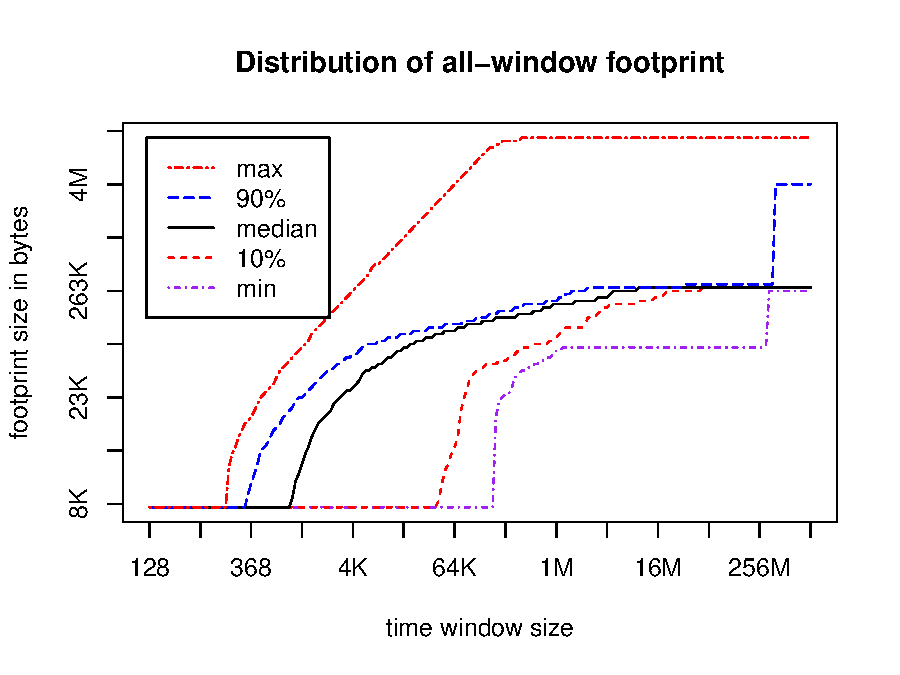
\includegraphics[width=\figwid]{figures/fp/164_gzip_ref}
    \label{fp-gzip-128}
  }\hfill \subfigure[{\bf Bzip2} has a larger working set than
  \emph{Gzip} for windows larger than 256 thousand accesses.] {
    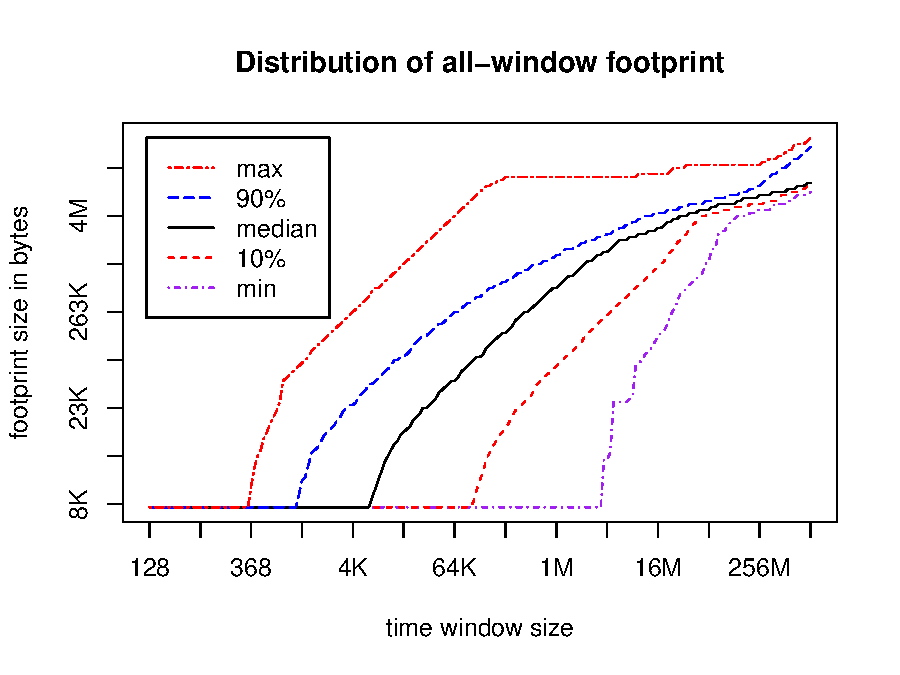
\includegraphics[width=\figwid]{figures/fp/256_bzip2_ref}
    \label{fp-bzip2-128}
  }\hfill
  \subfigure[{\bf Equake} has a streaming access pattern.  The
  footprint increases linearly with the window size.]{
    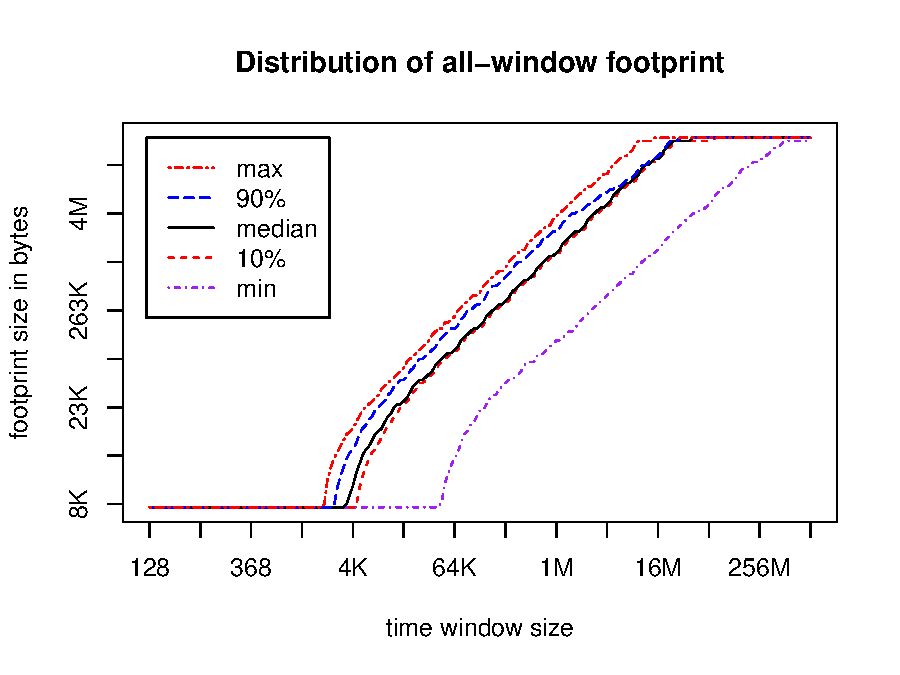
\includegraphics[width=\figwid]{figures/fp/183_equake_ref}
    \label{fp-equake-128}
  }\hfill \subfigure[{\bf Twolf} shows a narrow distribution ---80\%
  windows of the same length have nearly the same footprint. ]{
    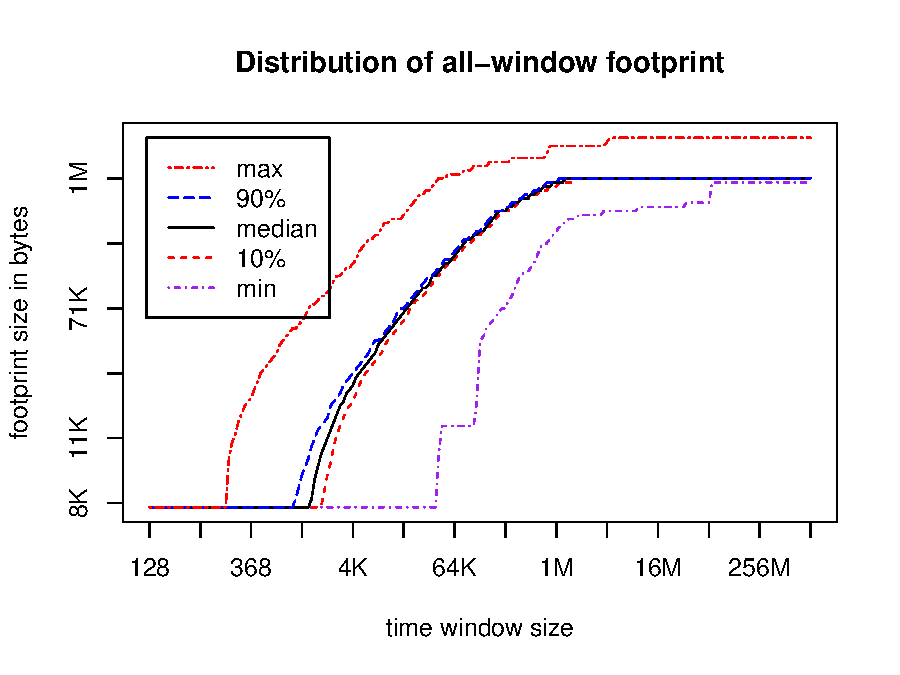
\includegraphics[width=\figwid]{figures/fp/300_twolf_ref}
    \label{fp-twolf-128}
  }\hfill
  \caption{The distribution of all-window footprint shows the
    characteristics of the working set in 4 SPEC2000 benchmarks.}
  \label{fig:all-fp-group}
\end{figure}

The footprint distribution shows highly summarized information about
program data usage.  For example, every point $<x,y>$ in the {\tt min} curve
shows the minimal footprint in all windows of size $x$ is $y$.  
As a sanity check, a reader can verify that the minimal and the
maximal footprints are monotone functions of the window size.  The
monotonicity should hold in theory but in an observation, it is not
guaranteed if we sample a set of windows rather than measure all
windows.

All-window footprint shows the characteristics of the working sets in
a program.  \emph{Gzip} has constant-size median working sets for
windows from 1 million to 256 million accesses, shown by
Figure~\ref{fp-gzip-128}.  In compression or decompression, the same
data buffers are repeatedly used for each chunk of the input or output
file.  Constant-size working sets are a result of complete data reuse.
\emph{Bzip2} creates larger auxiliary data structures in order to
improve compression ratio over a larger scope.  Its working sets
increase in size with the length of the execution window.  The rate of
increase, however, gradually decreases, as shown by
Figure~\ref{fp-bzip2-128}.

Shown in Figure~\ref{fp-equake-128}, {\tt Equake} has the clear
streaming access pattern because its working set size increases
linearly with the execution window length.  In fact, it shows the most
rapid growth, resulting in the largest footprint among all programs we
have tested.  90\% of footprints increase from 8KB to 8MB when window
size increases from 30K to 32M data accesses.  Its footprint
interferes with many other programs when running in shared cache.
{\tt Twolf} in Figure~\ref{fp-twolf-128} shows the smallest variation
in footprint size.  80\% of windows have nearly the
same size footprint.  These examples show that 
applications have different characteristics in their footprint distribution.

\paragraph{Measurement speed}
We have tested 12 SPEC2000 benchmark programs with the reference inputs. 
The length of the traces range from 4 billion to 108 billion, the size
of data ranges from 7 thousand to 787 thousand cache lines(64B), the number of
intervals ranges from 1.8 million to 48 billion, the average interval
length ranges from 504 to 19 thousand, and the measurement speed
ranges from 264 thousand data accesses per second to 8.4 million
accesses per second.  If we measure in terms of the number of windows
measured, the speed ranges from $10^{15}$ (a quadrillion) windows per
second to nearly $10^{18}$ (a quintillion) windows per second.

The speed closely correlates with the average interval length.  The
average length of $k$ means that in a random time window, 128 distinct
data elements are accessed by each $k$ accesses.  When the length is
500, the measurement speed is less than 300 thousand accesses per
second.  However, when the length is 19,000, the speed becomes 7.3
million accesses per second.  The average length is determined by the
length of the trace and the number of intervals.  Hence the cost of
the algorithm is determined by the number of intervals, $K$, more than
any other factor.

%to do: which input is used? test or ref? why it's said ref before and
%now it becomes test input
\paragraph{Comparison between CKlogM and NlogM}
The NlogM algorithm was the first to attempt complete all-window
measurement~\cite{DingC:PPOPP08}.  Here we compare NlogM with
CKlogM for $C=128$ and $C=256$.  Table~\ref{tbl:all-fp-time-compare} shows
the result of 14 SPEC2K benchmarks (that the NlogM method could finish
analyzing), including the length of the trace,
the size of data, the measurement time by NlogM, and the speedup
numbers by CKlogM for two Cs.  We have to use test inputs for comparison because it
takes too long for NlogM to measure larger inputs.  The measurement
time ranges from 414 seconds for \emph{mcf} to 4 hours
for \emph{parser} by NlogM and from 3 and 2 seconds for \emph{twolf}
to 18 and 17 minutes for \emph{ammp} by CKlogM when $C=128$ and
$C=256$.  The largest reduction is a factor of 316 for \emph{twolf}
from 10 minutes to 2 seconds.  The smallest reduction is a factor of 8
for \emph{mcf} from 7 minutes to 53 seconds. 

\begin{table}[h]
\small
\centering
\begin{tabular}{|l|c|c|c|c|c|c|c|}
\hline
prog. & $N$ & $M$ & NlogM & CKlogM C=128  & CKlogM C=256  \\ 
        &     &     & time[sec]  & time(speed) & time(speed) \\ \hline \hline
gzip    & 804M & 9K  & 12K   & 328(35)  & 246(47) \\ \hline
vpr     & 298M & 5K & 4K    & 84(49)  & 41(90) \\ \hline
gcc     & 255M & 15K  & 4K   & 37(102) & 19(198) \\ \hline
mesa    & 173M & 25K  & 2.6K  & 10(259) & 9(288) \\ \hline
art     & 1.0B  & 5K  & 12K   & 119(104) & 108(114) \\ \hline \hline
mcf     & 40M & 5K & 414   & 52(7.8) & 41(10) \\ \hline
equake  & 342M & 40K  & 5K    & 42(126) & 33(161) \\ \hline
crafty  & 935M & 8K & 15K   & 739(20)  & 187(78) \\ \hline
ammp    & 818M & 51K & 13K   & 1129(12)  & 1036(13) \\ \hline
parser  & 929M & 24K & 14K  & 142(101) & 98(147) \\ \hline \hline
gap     & 277M & 147K & 5K    & 30(168) & 20(252) \\ \hline
twolf   & 76M  & 309 & 631   & 3(210) & 2(316) \\ \hline \hline
median  & 320M & 12K & 5178 & 68({\bf 101}) & 41({\bf 131}) \\ \hline
mean    & 497M & 28K & 7343 & 226({\bf 100}) & 153({\bf 143}) \\ \hline
\end{tabular}
\caption{Time comparison for the test input of 12 SPEC 2K benchmarks.  On average, the measurement time is reduced from 2 hours per program to 73 and 52 seconds when $C=128$ and $256$ respectively. }
\label{tbl:all-fp-time-compare}
\end{table}

The average statistics is shown at the bottom of
Table~\ref{tbl:all-fp-time-compare}.  On average across 12 benchmarks, the
length of the trace is half billion memory accesses and the size of
data is 28 thousand words.  The average measurement time of NlogM is
two hours.  The average reduction by CKlogM is a factor of 100 to 73
seconds when $C=128$ and a factor of 142 to 52 seconds when $C=256$.
In other words, \emph{CKlogM reduces the average measurement time from
two hours to one minute.}

% Two programs, bzip2 and gzip, have different size footprints, which suggests that programs running with gzip have much less cache interference than when they are run with bzip.

\paragraph{Relation between $c$ and measurement speedup}
We define the \emph{speedup factor} by $\frac{N}{CK}$.  Intuitively, a
larger $c$ produces a greater speedup.  However, this is not true.  We
have measured all power-of-two $c$ values for all our tests and
studied the relation between $c$ and the potential speedup.  When the
speedup numbers for different $c$ were drawn as a curve, we have
observed variations in terms of whether a curve has a single peak or
whether the shape changes when a program is run with different inputs.
Figure~\ref{fig:ck-speedups} show the speedup factor for 4 programs whose
footprint we have shown in Figure~\ref{fig:all-fp-group}.  The highest
%speedup is in tens of thousands for {\em bzip2} a\cund {\em gzip}, one
speedup is in tens of thousands for {\tt bzip2} and {\tt gzip}, one
hundred thousand for {\tt equake}, and (too large to shown in the
figure) 1.6 million for {\tt twolf}.

\begin{figure}[h]
\centering
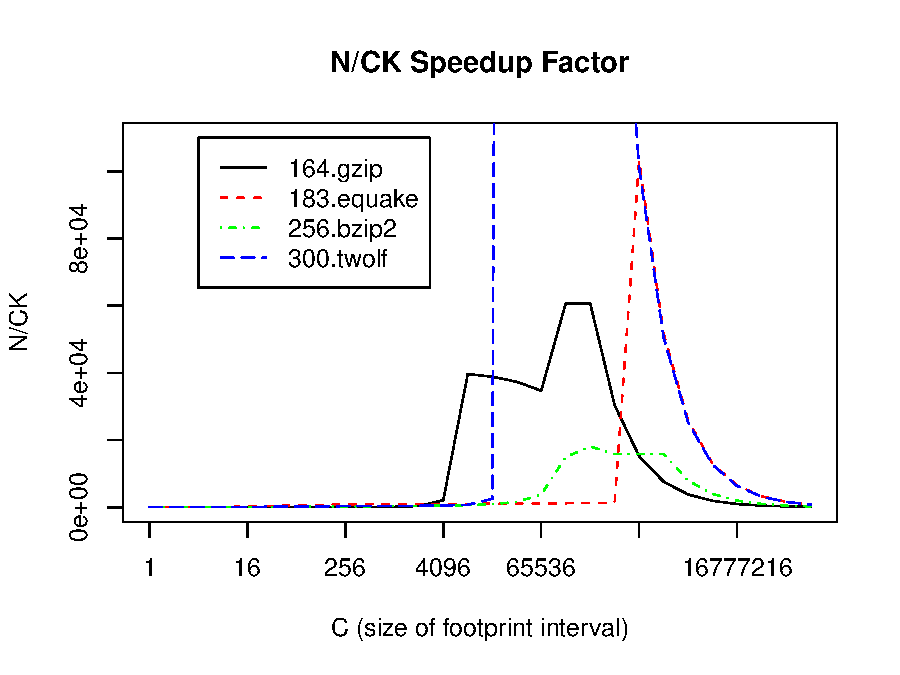
\includegraphics[width=0.7\textwidth]{figures/fp/ck}
\caption{$\frac{N}{CK}$ gives the speedup factors for 4 SPEC CPU2000
  benchmarks.  The speedup factors for {\tt twolf} are as high as 1.6
  million but are not shown above 100K in order to make other numbers
  easy to see.}
\label{fig:ck-speedups}
\end{figure}

\paragraph{Comparison with Miss Count}
It is interesting to consider the relation between the number of
misses in a window and the footprint of the window.  On average, the
number of misses is the miss rate times the window size.  Therefore,
the average miss count grows linearly.  It is unbounded if a program
executes forever.  The footprint is bounded by the size of program
data.  The growth cannot be always linear.

This difference is shown in the example of \emph{Gzip} result in
Figure~\ref{fig:miss-fp-comp}.  The miss count should be in the unit of
64-byte blocks.  The figure shows it in bytes growing linearly from
$2^{-9}$ byte to $2^{26}$ (83MB or 1.3 million misses) for window
sizes ranging from 1 access to 18 billion.  For the same window sizes,
the footprint grows from 64 bytes (1 block) to 83MB.  This difference
leads to different predictions of cache interference.  We compare
the accuracy of these predictions in cache sharing models, which will
be investigated in Chapter~\ref{chap:corun}.

\begin{figure}[h]
\centering
\includegraphics[width=0.7\textwidth]{figures/fp/miss_fp_comp}
\caption{Comparison of linear miss count growth and non-linear
  footprint growth in \emph{Gzip}.}
\label{fig:miss-fp-comp}
\end{figure}


\subsection{Efficiency of Average-footprint Analysis}
\label{subsec:fp-eval-aver-fp}
We have implemented the average-footprint analysis algorithm in a
Pin-based profiling tool
and tested 26 SPEC2K benchmarks, 12 integer and 14 floating-point,
and 29 SPEC2006 benchmarks, 12 integer and 17 floating-point. All
benchmarks are instrumented by Pin~\cite{Pin:PLDI05} and different
benchmarks are profiled on a linux cluster in parallel, with each node
has two 3.2GHz 64-bit Intel Xeon processors with 1MB L2 cache each and
6GB physical memory total.
\begin{comment}
a machine with an Intel Core i5-660 processor and 4GB physical
memory. The machine is installed with Fedora 13 and GCC 4.4.5.
\end{comment}

\paragraph{Average footprint overview}
Figure~\ref{fig:aver-fp-bzip2} shows an example average footprint
graph of bzip2 from SPEC2006 benchmark suite. The graph shows window
size, measured in number of data accesses with linear scale, in
$x$-axis and average footprint, measured in kilo-bytes, in the
$y$-axis. Since our measurements are based on 64-byte blocks, the
footprint sizes are always multiples of 64. At each window size, there
is one and only one average footprint value corresponding to the window
size. We connect all the average footprint points into a line, and
name the line {\em average footprint curve}. For each run of a
sequential program with a given input, only one average footprint curve
exists for this run.

\begin{figure}[!h]
  \centering
  \includegraphics[width=0.7\textwidth]{figures/fp/401_bzip2_fp}
  \caption{The average footprint curve for SPEC20006/bzip2 with
    the first reference input.}
  \label{fig:aver-fp-bzip2}
\end{figure}

\paragraph{Measurement speed}
Table~\ref{tbl:aver-fp-speed} summarizes the analysis cost for the two
benchmark suites, and for each suite, the average for integer and for
floating-point programs.  It divides the 55 tests into four groups: 12
SPEC 2000 integer programs, 14 SPEC 2000 floating-point programs, 12
SPEC 2006 integer programs, and 17 SPEC 2006 floating-point programs.
The result of each group is summarized in three rows and three
columns.  The columns show the trace length, the data size, and the
slowdown ratio of the profiling time to the unmodified run time.  The
rows show the minimum, maximum, and the average slowdown factors for all benchmarks
of the group.

\begin{table*}[!h]
\centering
\small
\begin{tabular}{|c|c|c|c|c|}
\hline
benchmarks        &  stats     &trace length   &data size(64B lines)   &avg-FP slowdown(X) \\ \hline \hline
{\bf SPEC2000 INT}     & min   & 1.41 E+10     & 0.13 E+5      & 8.8 \\\cline{2-5}
    12  programs   & max   & 16.05 E+10    & 32.55 E+5     & 39.7 \\ \cline{2-5}
       & mean          & 7.52 E+10     & 11.67 E+5     & 28.8 \\ \hline \hline
{\bf SPEC2000 FP}      & min   & 3.03 E+10     & 0.56 E+5      & 9.7 \\ \cline{2-5}
    14   programs    & max   & 42.55 E+10    & 31.28 E+5     & 32.4 \\ \cline{2-5}
      & mean          & 17.44 E+10    & 14.16 E+5     & 21.9 \\ \hline \hline
{\bf SPEC2006 INT}     & min   & 4.88 E+10     & 3.01 E+5      & 8.1 \\ \cline{2-5}
     12  programs    & max   & 151.47 E+10   & 137.36 E+5    & 40.9 \\ \cline{2-5}
      & mean          & 47.20 E+10    & 34.05 E+5     & 20.7 \\ \hline \hline
{\bf SPEC2006 FP}      & min   & 20.73 E+10    & 0.40 E+5      & 9.4 \\ \cline{2-5}
      17   programs  & max   & 385.15 E+10   & 145.03 E+5    & 73.9 \\ \cline{2-5}
      & mean          & 138.85 E+10   & 58.69 E+5     & 26.1 \\ \hline
\end{tabular}
\caption{The min, max, and average costs (slowdowns) of average-footprint analysis for 55 SPEC 2000 and SPEC 2006 benchmark programs}
\label{tbl:aver-fp-speed}
\end{table*}

The minimum slowdowns in four benchmark groups are all below 10.  The
maximum slowdowns are 40, 32, 41, and 74.  The average slowdowns are between
21 in SPEC 2006 integer tests and 29 in SPEC 2000 integer tests.  On
average across all four groups, average-footprint analysis takes no more
than 30 times of the original execution time.

The individual results of the 29 SPEC2006  programs are not included in 
Table~\ref{tbl:all-times-spec2k} and Table~\ref{tbl:all-times-spec06}.
%Table~\ref{tbl:spec06-int-basic} and
%Table~\ref{tbl:spec06-fp-basic}. 
On average, an unmodified SPEC 2000 program (the original
program without any instrumentation or analysis) takes less than
3 minutes, and an unmodified SPEC 2006 program takes close to 10 minutes.
Average-footprint analysis takes 3 to 73 minutes for SPEC 2000
programs and 10 minutes (\emph{gcc}) to 10 hours (\emph{calculix}) 
for SPEC 2006 programs.


\paragraph{Comparison with All-footprint Analysis}

All-footprint analysis can analyze SPEC 2000 programs but not SPEC
2006 programs.  We compare average- and all-footprint analysis on SPEC
2000 programs in Table~\ref{tbl:all-aver-compare}. The table summarizes the
cost of the two analyses in these 15 tests in the last two columns.  The slowdowns by
average-footprint analysis are between 8.8 and 40.  The slowdowns by
all-footprint analysis are between 248 and 3160.  The average slowdown
is 40 for average-footprint analysis and about 1500 for all-footprint
analysis.  In other words, on average for these 15 programs,
average-footprint analysis is 38 times faster than all-footprint
analysis.

\begin{table*}[!h]
\small
\centering
\begin{tabular}{|c|c|c|c|c|c|c|c|c|c|c|}
\hline
{\bf 15 SPEC2000}       &trace length   &data size   &avg-FP &all-FP \\ 
{\bf Benchmarks}        &             &(Bytes)   &slowdown(X) &slowdown(X) \\ \hline \hline
min   & 1.41 E+10     & 1.98 E+6      & 8.8  & 248.2\\ \hline
max   & 16.05 E+10    & 2.08 E+8     & 39.7 & 3160.5\\ \hline
mean  & 8.20 E+10     & 6.43 E+7     & 26.1 & 1495.2\\ \hline 
\end{tabular}
\caption{Comparison of the min, max, and average slowdowns by average-footprint analysis and by all-footprint analysis.  On average, average-footprint analysis is 38 times faster.}
\label{tbl:all-aver-compare}
\end{table*}

All-footprint analysis takes too long for SPEC 2006 programs.  For
example, it takes average-footprint analysis 10 hours to profile
\emph{calculix}.  If all-footprint analysis is 38 times slower, it
would take more than two weeks to finish the same analysis.


\subsection{Efficiency of Footprint Sampling}
\label{sec:samp-result}

For this experiment, we choose somewhat arbitrarily the frequency
of one sample every 10 seconds.  The sample length depends on how
fast the footprint reaches cache size. 
In Table~\ref{tbl:sampling-fp-speed}, we 
show the slowdown of footprint sampling in the end-to-end run time by the
column marked $FP\-sampling\ slowdown$.  It ranges from 0\% to
2.14\%. Three programs have a visible cost of over 1\%.  They are
\emph{bwaves} 2.1\%, \emph{GemsFDTD} 1.3\% and \emph{milc} 1.5\%.  The
reason for the relatively high cost may be the non-trivial
interference between the sampling task and the parent task.  Across
all programs, the average visible overhead is below a half percent.
If we measure the total CPU time, sampling takes between 0\% and 80\%
of the original run time.  The average cost is 19\%, of which
over 18\% is hidden by shadow profiling.  The coverage is computed by the ratio of the number of
sampled instructions to the total number of instructions (counted by
our full trace profiling).  The coverage is as low as 0.006\% in
\emph{lbm}.

\begin{comment}
for calculation:
a = [4.2, 1.7, 0.2, 1.2, 0.9, 4.9, 7, 3, 2.6, 1.4, 14.4, 4.8, 3.8, 5.7, 20.6, 6.8, 6.8, 4.8, 9.5, 8.6, 3.3, 8.9]
\end{comment}

\begin{table}[!h]
\centering
\begin{tabular}{|c|c|c|c|c|c|}
\hline
{\bf 22 SPEC2006} &trace length &data size & FP-sampling & coverage \\ 
{\bf Benchmarks} &              &(bytes) & slowdown(\%) & (\%)\\\hline \hline
min & 0.2 E+11 & 0.3 E+7 & 0.00 & 0.01 \\ \hline
max & 20.6 E+11 & 175.7 E+7 & 2.14 & 3.1\\ \hline
mean & 5.69 E+11 & 36.96 E+7 & 0.47 & 0.94\\ \hline
\end{tabular}
\caption{Min, max, and average slowdowns by average-footprint sampling.  On average, sampling incurs only 0.47\% overhead.}
\label{tbl:sampling-fp-speed}
\end{table}


\section{Discussion}

We have presented the first accurate all-window footprint analysis,
CKlogM all-footprint analysis.
The new algorithm combines relative precision
approximation and trace compression to reduce the asymptotic cost to
$O(CKlogM)$.  We have successfully measured all-window footprints in
the SPEC2K benchmark suite in its full-length executions.  It is the
first time such complete measurement is made.  The results show that
applications differ in their footprints in terms of not just the size
but also the relation with time and the compactness of the
distribution.  The previous fastest accurate method, O(NlogM)
algorithm, could only measure these programs on their test input, for
which the new algorithm reduces the profiling time from 2 hours to 1
minute.  The all-window analysis measures a quadrillion to nearly a
quintillion footprints per second.

Although CKlogM algorithm have significantly reduced the measurement
time, the cost is still too high for real-size workloads. We
introduces a technique, average-footprint analysis, for measuring the
average footprint size. By confining the analysis to the average
rather than the full range, the 
problem  can be solved accurately by a linear-time algorithm.
The linear-time algorithm uses differential counting based on the
forward and backward reuse time distance.  When tested on SPEC CPU
2000 and 2006 benchmark suites, the average slowdowns are between 20
to 29, and the new linear-time algorithm is 38 times faster than
all-window footprint analysis. 

To make footprint an online measurable metric, we apply shadow
sampling to average-footprint analysis. Sampling reduces the visible
profiling overhead to around 0.47\%. While approximation and sampling
greatly reduce the profiling overhead, there is no guarantee that they
will preserve all the information. Whether the information captured is
representative of the whole program is the key to the usefulness of
all these techniques. We will evaluate all-footprint analysis,
average-footprint analysis, and shadow sampling in locality
models(Chapter~\ref{chap:model}) and cache sharing
models(Chapter~\ref{chap:corun}), and prove their contributions in real
use. 



\begin{table}[h]
\centering
\footnotesize
\begin{tabular}{|l|c|c|c|c|c|c|}
\hline
benchmark        &trace   &data size   &unmodified  &avg-FP &FP alg \\ 
&length &(64B lines) &time(sec) &time(sec) &cost(X)\\ \hline \hline
164.gzip         & 3.93 E+10     & 14.07 E+5     & 22.7          & 460.0         & 20.3 \\ \hline
175.vpr          & 6.26 E+10     & 0.38 E+5      & 33.7          & 809.0         & 24.0 \\ \hline
176.gcc          & 1.41 E+10     & 32.55 E+5     & 4.7   & 187.0         & 39.7 \\ \hline
181.mcf          & 2.29 E+10     & 12.62 E+5     & 46.6          & 408.0         & 8.8 \\ \hline
186.crafty       & 11.36 E+10    & 0.32 E+5      & 37.2          & 1427.0        & 38.4 \\ \hline
197.parser       & 16.05 E+10    & 4.11 E+5      & 80.2          & 1926.0        & 24.0 \\ \hline
252.eon          & 7.18 E+10     & 0.13 E+5      & 20.1          & 786.0         & 39.2 \\ \hline
253.perlbmk      & 4.69 E+10     & 18.14 E+5     & 14.9          & 542.0         & 36.3 \\ \hline
254.gap          & 11.16 E+10    & 31.50 E+5     & 39.4          & 1261.0        & 32.0 \\ \hline
255.vortex       & 6.45 E+10     & 10.92 E+5     & 19.7          & 770.0         & 39.0 \\ \hline
256.bzip2        & 4.72 E+10     & 14.71 E+5     & 23.4          & 548.0         & 23.4 \\ \hline
300.twolf        & 14.74 E+10    & 0.60 E+5      & 93.8          & 1917.0        & 20.4 \\ \hline
\hline
168.wupwise      & 15.68 E+10    & 28.82 E+5     & 112.8         & 1695.0        & 15.0 \\ \hline
171.swim         & 9.02 E+10     & 31.21 E+5     & 99.7          & 1141.0        & 11.4 \\ \hline
172.mgrid        & 42.55 E+10    & 9.10 E+5      & 175.2         & 4395.0        & 25.1 \\ \hline
173.applu        & 18.47 E+10    & 28.57 E+5     & 68.0          & 1999.0        & 29.4 \\ \hline
177.mesa         & 15.85 E+10    & 1.37 E+5      & 56.1          & 1799.0        & 32.1 \\ \hline
178.galgel       & 39.75 E+10    & 8.47 E+5      & 135.8         & 4397.0        & 32.4 \\ \hline
179.art          & 3.03 E+10     & 0.56 E+5      & 48.2          & 470.0         & 9.7 \\ \hline
183.equake       & 6.87 E+10     & 6.80 E+5      & 33.5          & 774.0         & 23.1 \\ \hline
187.facerec      & 14.62 E+10    & 2.98 E+5      & 63.7          & 1623.0        & 25.5 \\ \hline
188.ammp         & 14.26 E+10    & 2.14 E+5      & 84.4          & 1738.0        & 20.6 \\ \hline
189.lucas        & 15.07 E+10    & 25.95 E+5     & 63.9          & 1685.0        & 26.4 \\ \hline
191.fma3d        & 16.04 E+10    & 17.06 E+5     & 82.6          & 1854.0        & 22.4 \\ \hline
200.sixtrack     & 14.20 E+10    & 3.94 E+5      & 133.0         & 1608.0        & 12.1 \\ \hline
301.apsi         & 18.69 E+10    & 31.28 E+5     & 102.2         & 2218.0        & 21.7 \\ \hline
\end{tabular}
\caption{Individual statistics of the 26 SPEC2000 test programs}
\label{tbl:all-times-spec2k}
\end{table}

\begin{table}[h]
\centering
\footnotesize
\begin{tabular}{|l|c|c|c|c|c|c|}
\hline
benchmark        &trace   &data size   &unmodified  &avg-FP &FP alg \\ 
&length &(64B lines) &time(sec) &time(sec) &cost(X)\\ \hline \hline
400.perlbench    & 21.99 E+10    & 52.31 E+5     & 222.3         & 2478.0        & 11.1 \\ \hline
401.bzip2        & 9.73 E+10     & 11.98 E+5     & 129.4         & 1051.0        & 8.1 \\ \hline
403.gcc          & 4.88 E+10     & 41.74 E+5     & 31.5          & 594.0         & 18.8 \\ \hline
429.mcf          & 21.61 E+10    & 137.36 E+5    & 338.3         & 3627.0        & 10.7 \\ \hline
445.gobmk        & 12.48 E+10    & 3.06 E+5      & 67.0          & 1458.0        & 21.8 \\ \hline
456.hmmer        & 68.40 E+10    & 6.61 E+5      & 178.8         & 6441.0        & 36.0 \\ \hline
458.sjeng        & 110.99 E+10   & 28.56 E+5     & 518.8         & 12906.0       & 24.9 \\ \hline
462.libquantum   & 151.47 E+10   & 20.99 E+5     & 633.3         & 14930.0       & 23.6 \\ \hline
464.h264ref      & 41.10 E+10    & 3.01 E+5      & 99.5          & 4075.0        & 40.9 \\ \hline
471.omnetpp      & 40.77 E+10    & 16.44 E+5     & 422.2         & 5797.0        & 13.7 \\ \hline
473.astar        & 29.57 E+10    & 35.99 E+5     & 229.1         & 3396.0        & 14.8 \\ \hline
483.xalancbmk    & 53.38 E+10    & 50.50 E+5     & 297.9         & 6943.0        & 23.3 \\ \hline
\hline
410.bwaves       & 190.51 E+10   & 145.03 E+5    & 555.4         & 18551.0       & 33.4 \\ \hline
416.gamess       & 144.61 E+10   & 0.52 E+5      & 212.2         & 15682.0       & 73.9 \\ \hline
433.milc         & 51.48 E+10    & 113.33 E+5    & 565.8         & 5852.0        & 10.3 \\ \hline
434.zeusmp       & 85.62 E+10    & 81.21 E+5     & 593.1         & 9584.0        & 16.2 \\ \hline
435.gromacs      & 130.60 E+10   & 2.22 E+5      & 853.8         & 12883.0       & 15.1 \\ \hline
436.cactusADM    & 230.01 E+10   & 102.33 E+5    & 1297.5        & 24751.0       & 19.1 \\ \hline
437.leslie3d     & 112.12 E+10   & 20.18 E+5     & 578.2         & 11546.0       & 20.0 \\ \hline
444.namd         & 117.12 E+10   & 7.36 E+5      & 501.7         & 11799.0       & 23.5 \\ \hline
447.dealII       & 109.73 E+10   & 88.48 E+5     & 417.3         & 12542.0       & 30.1 \\ \hline
450.soplex       & 20.73 E+10    & 76.33 E+5     & 236.3         & 2219.0        & 9.4 \\ \hline
453.povray       & 67.91 E+10    & 0.40 E+5      & 227.9         & 7134.0        & 31.3 \\ \hline
454.calculix     & 385.15 E+10   & 27.92 E+5     & 755.2         & 36728.0       & 48.6 \\ \hline
459.GemsFDTD     & 155.60 E+10   & 136.10 E+5    & 714.4         & 15719.0       & 22.0 \\ \hline
465.tonto        & 146.23 E+10   & 6.45 E+5      & 640.1         & 15280.0       & 23.9 \\ \hline
470.lbm          & 79.73 E+10    & 67.03 E+5     & 430.8         & 8645.0        & 20.1 \\ \hline
481.wrf          & 200.09 E+10   & 116.40 E+5    & 866.4         & 21419.0       & 24.7 \\ \hline
482.sphinx3      & 133.24 E+10   & 6.43 E+5      & 679.6         & 14750.0       & 21.7 \\ \hline

%\hline
\end{tabular}
\caption{Individual statistics of the 29 SPEC2006 test programs}
\label{tbl:all-times-spec06}
\end{table}

\begin{comment}
\begin{table}
\centering
\begin{tabular}{|l|c|c|c|c|}
\hline
$bench name$ & $n$ $(10^{11})$ & $m$ $(10^7 bytes)$ & $T(sec)$ \\ \hline \hline 
400.perlbench & 4.2 & 24.4 & 457 \\ \hline
401.bzip2 & 1.7 & 39.3 & 263 \\ \hline
403.gcc & 0.2 & 40.4 & 72 \\ \hline
429.mcf & 1.2 & 175.7 & 1172 \\ \hline
445.gobmk & 0.9 & 2.7 & 173 \\ \hline
456.hmmer & 4.9 & 4.2 & 303 \\ \hline
458.sjeng & 7.0 & 18.2 & 1356 \\ \hline
462.libquantum & 3.0 & 16.8 & 1391 \\ \hline
464.h264ref & 2.6 & 2.7 & 143 \\ \hline
471.omnetpp & 2.3 & 17.6 & 1048 \\ \hline
473.astar & 1.4 & 29.5 & 512 \\ \hline
483.xalancbmk & 3.6 & 43.8 & 778 \\ \hline
\end{tabular} 
\caption{The SPEC2006 integer benchmarks. 
For each benchmark, $n$ is the memory trace length of whole execution, $m$ is 
the number of distinct data blocks (size in bytes) accessed during the execution, and $T$ is the
execution time without any instrumentation or analysis.}
\label{tbl:spec06-int-basic}
\end{table}

\begin{table}
\centering
\begin{tabular}{|l|c|c|c|c|}
\hline
$bench name$ & $n$ $(10^{11})$ & $m$ $(10^7 bytes)$& $T(sec)$ \\ \hline \hline 
410.bwaves & 14.4 & 98.2 & 1664 \\ \hline
416.gamess & 4.8 & 0.3 & 444 \\ \hline
433.milc & 3.8 & 74.2 & 1077 \\ \hline
434.zeusmp & 5.7 & 51.9 & 1555 \\ \hline
435.gromacs & 9.8 & 1.4 & 1272 \\ \hline
436.cactusADM & 20.6 & 65.5 & 3411 \\ \hline
437.leslie3d & 6.8 & 12.9 & 1212 \\ \hline
444.namd & 6.8 & 4.7 & 915 \\ \hline
447.dealII & 7.3 & 88.5 & 773 \\ \hline
450.soplex & 1.0 & 16.2 & 604 \\ \hline
453.povray & 4.8 & 0.3 & 493 \\ \hline
454.calculix & 9.5 & 16.4 & 1512 \\ \hline
459.GemsFDTD & 8.6 & 86.9 & 1397 \\ \hline
465.tonto & 10.0 & 5.2 & 1312 \\ \hline
470.lbm & 3.3 & 42.9 & 1491 \\ \hline
481.wrf & 9.7 & 76.8 & 1895 \\ \hline
482.sphinx3 & 8.9 & 5.1 & 1765 \\ \hline
\end{tabular} 
\caption{The SPEC2006 floating-point benchmarks. 
For each benchmark, $n$ is the memory trace length of whole execution, $m$ is 
the number of distinct data blocks (size in bytes) accessed during the execution, and $T$ is the
execution time without any instrumentation or analysis.}
\label{tbl:spec06-fp-basic}
\end{table}
\end{comment}


\chapter{A Higher Order Theory of Locality}
\label{chap:model}

An influential theory developed over the past four decades is the
working-set theory (WSLT)~\cite{Denning:TSE80}. In this chapter, we
develop a similar theory for cache locality (CLT), a higher order
theory of locality which connects five different locality metrics,
footprint, inter-miss time, volume fill time, miss ratio, and reuse
distance. The theory includes a series of conversion methods and their
correctness condition. We refer to the new theory as HOTL(a {\bf
  H}igher {\bf O}lder {\bf T}heory of {\bf L}ocality) theory and refer
to these methods collectively as the HOTL conversion for the five
metrics.

Footprint plays an important role in HOTL theory. The fact that
HOTL theory endows each of the five cache locality metrics the
collective strength of all its Filmer peers makes footprint's strength,
such as measuring efficiency and composibility, available to all other
metrics. HOTL theory can be used in many locality related fields, such
as locality measurement, prediction, and optimizations, in both
standalone and multi-tasks environments. 

\section{Introduction}
The memory system of a computer is organized as a hierarchy.  Locality
metrics are used in software and hardware to manage and optimize the
use of the memory hierarchy.  For locality analysis, the basic unit of
information is a data access, and the basic relation is a data reuse.
The theory of locality is concerned with the fundamental properties of
data accesses and reuses, just as the graph theory is with nodes and
their links.

Cache locality metrics are many and varied.  To quantify performance,
we use the miss rate.  To manage sharing, we use the footprint.  To
analyze and optimize a program, we use the reuse distance.  Some
metrics are hardware dependent, useful for evaluating a specific
machine and managing it at run time.  Others are hardware independent,
useful for optimizing a program for all cache sizes.  The two types of
metrics are converging in multicore caching, where the total cache
size is fixed but the available portion for each program varies. 

In this chapter we consider five locality metrics, with a short description
here and the precise definitions in the next section.

\begin{itemize}
\item \emph{Footprint}: the expected amount of data a program accesses
  in a given length window.
\item \emph{Inter-miss time}: the average time between two cache
  misses in a given size cache.
\item \emph{Volume fill time}: the average time for the program to
  access a given volume of data.
\item \emph{Miss ratio}: the fraction of references that cause cache
  misses.
\item \emph{Reuse distance}: for each data access, the amount of data
  accessed between this and the previous access to the same datum.
\end{itemize}

\noindent To denote them collectively, we insert `et' between the last
two,  take the initial letters (except for the fill time from which we
take one 'l'), and produce the acronym ``Filmer''. 

We present a theory showing that the five Filmer
metrics can be mutually derived from each other.  The conversion
involves taking the difference in one direction and the sum in the
reverse direction.  The theoretical relation is analogous to
differentiation and  integration.  Hence we call it a \emph{higher
  order theory} of locality (HOTL).

Similar conversions have been part of the working set theory, making
it the first HOTL theory (Section~\ref{sec:Denning}).  The working set
theory was developed to analyze locality in the main memory.  The new
theory we develop is for cache memory.  It endows each of the five cache locality
metrics the collective strength of all its Filmer peers:

\begin{itemize}
\item \emph{Efficiency}.  If we can measure one
  Filmer metric on-line, we can calculate all the others at the same
  time.
\item \emph{Composability}.  The miss rate does not compose in that
  when a group of programs are run together, the number of misses is
  not the sum of the misses of each member running alone.  If another
  Filmer metric is composable, then we can compose the miss rate
  indirectly.
\item \emph{Hardware sensitivity}.  If we can measure the effect of
  cache associativity and other hardware parameters on the miss rate,
  we can compute their impact on the other metrics.
\end{itemize}

The conversion methods we describe are not always accurate.  The
correctness depends on whether the footprint statistics in reuse
windows is similar to the footprint in general windows, in other
words, whether the reuse windows are representative of general
windows.  We call the condition the \emph{reuse-window hypothesis}.
The Filmer metrics capture different aspects of an execution: the
reuse distance is per access, the footprint is per window, while the
miss-ratio has the characteristics of both. Their conversion creates
conflicts, and the reuse-window hypothesis is the condition
for reconciliation.

We apply the HOTL theory to convert footprint to reuse distance and predict
the miss ratio. The purpose of the miss-ratio prediction is twofold:
to validate the theory and to show a practical value. The main results
are: 

\begin{itemize}
\item \emph{Real-time locality measurement.}  The HOTL-enabled
  technique predicts the miss ratio for thousands of cache sizes with
  a negligible overhead.  When tested on SPEC 2006 and
  PARSEC parallel benchmarks, the prediction matches the actual miss
  ratio measured using the hardware counters.  Without sampling, the
  analysis is 39\% faster than simulating a single cache size.  With
  sampling, the end-to-end slowdown is less than 0.5\% on average with
  only three programs over 1\%.

\item \emph{Cache interference prediction.} The HOTL-enabled technique
  predicts the effect of cache sharing without parallel testing.  We
  will focus on cache sharing models and present the results of
  applying HOTL theory to cache interference prediction in Chapter~\ref{chap:corun}.
\end{itemize}

Knowing the miss rate does not mean knowing the memory performance.
The actual effect of a cache miss depends significantly on data
prefetching, memory-bus arbitration, and other factors either in the
CPU above the cache hierarchy or the main memory below.  In this
chapter, we limit our scope to the models of data and cache usage and to
methods that measure and reduce the number of cache misses.

\section{Locality Metrics}
\label{sec:metrics}

The working set theory defines the locality metrics to measure the
intrinsic demand of a process~\cite{Denning:CACM68}.   The actual
performance is the hardware response to the program demand.  By
defining locality metrics independent of their specific uses, the
approach combines clarity and concision on the one hand and usefulness
and flexibility on the other. We follow the same approach and say that
a locality metric is \emph{program intrinsic} if it uses only the
information from the data access trace of a program.  Throughout this
chapter, we use $n$ to denote the length of the trace and $m$ the
total amount of data accessed in the trace. 

A footprint is defined on a time window, and the miss ratio for a
cache size.  Since we do not know a priori in which window or
cache the metrics may be used, we define the footprint and miss ratio
metrics to include all windows and all cache sizes --- they are
functions over a parameter range.

The five metrics we consider are program intrinsic functions defined
on a sequential data access trace.  The time is logical and counted by
the number of data accesses from the start of the execution.  The
cache is fully associative and uses the LRU replacement, with a fixed
cache-block size.  We will consider the physical time and set
associative cache when we apply the basic theory in
Chapter~\ref{chap:corun}.  We use the term miss ratio if the time is
logical and miss rate if it is physical. 

\subsection{Average Footprint}

In this section we briefly review the concepts and algorithms we
introduced in Chapter~\ref{chap:fp}, a footprint is the amount of data
accessed in a time window.  A performance tool often measures it for
some execution window, i.e. taking a snapshot.  A complete measure
should consider \emph{all} execution windows.  For each length $t$,
the average footprint $fp(t)$ is the average footprint size in all
windows of length $t$. 

Let $W$ be the set of all length-$t$ windows in a length-$n$ trace.
Each window $w$ has a footprint $fp_w$. The average footprint $fp(t)$
is the total footprint in these windows divided by $n-t+1$, the number
of the length-$t$ windows. 

$$fp(t) = \frac{\sum_{all\ w\ of\ length\ t} fp_w}{n-t+1}$$

For example, the trace ``abbb'' has 3 windows of length 2: ``ab'',
``bb'', and ``bb''.  The size of the 3 footprints is 2, 1, and 1, so
$fp(2) = (2+1+1)/3 = 4/3$.  

The footprint is composable in that the combined footprint of two
programs is the sum of their individual footprints (assuming no data
sharing).  We will use this property when developing efficient models
of cache sharing in Chapter~\ref{chap:corun}. Another useful property,
which we have already explored in Section~\ref{sec:sampling}, is that
the footprint is amenable to sampling.

\subsection{Volume Fill Time}
\label{subsec:lf}

Intuitively, we may consider the cache as a reservoir and the data
access of a program a stream feeding into the reservoir with new
content.  Having a fixed capacity, the reservoir discharges (evicts)
previous volumes as it receives the new flows.  The key concept in
this analogy is the volume fill time, the time taken for a stream to
fill the reservoir.

The volume fill time is the time a program takes to access a given
amount of data, or symbolically, $vt(v)$ for volume $v$.  The metric
is program intrinsic.  To model hardware, we simplify and assume that
the cache is fully associative LRU.  Under the assumption, the volume
fill time $vt(c)$ is the time for a program to fill the cache of size
$c$.  Whether the cache is empty or not, after $vt(c)$, the cache
is populated with the data (and only the data) accessed in the last
$vt(c)$ time. In the cold-start cache, all data will be brought in by
cache misses. In the warm cache, the fraction of the data already in
the cache will stay, and the rest will be brought in by cache
misses. We call the volume fill time interchangeably as the
\emph{cache fill time}. 

The fill time can be defined in two different ways. First, we define
it as the inverse of the footprint function:

\begin{align*}
vt(c) = 
\begin{cases}
fp^{\ -1} (c) & \text{if } 0 \le c \le m \\
\infty & \text{if } c > m
\end{cases}
\end{align*}

\noindent where $m$ is the total amount of program data. Within the
range $0 \le c \le m$, the invariant $fp(vt(c)) = fp(fp^{\ -1}(c))= c$
symbolizes the conversion that when the footprint is the cache size,
the footprint window is the fill time. The conversion is shown
visually in Figure~\ref{fig:fp2vt}.  From the average footprint curve,
we find the cache size $c$ on the y-axis and draw a level line to the
right.  At the point the line meets the curve, the $x$-axis value is
the fill time $vt(c)$.

A careful reader may question the uniqueness of the fill time.  For
example for the trace ``xx...x'', it is unclear what should be the fill
time $vt(1)$.  When defined as the inverse function $fp^{-1}$, the same
problem happens if there are $x_1,x_2$ such that $fp(x_1) = fp(x_2)$.
However, this problem does not occur using the footprint-based
definition.  We will prove later in Section~\ref{sec:thm} that the
average footprint is a concave function.  As a result, it is strictly
increasing, and as its inverse, $vt$ is a proper function and strictly
increasing as well.  We call the footprint-based
definition the \emph{Filmer fill time}.

\begin{figure}[t!]
\centering
\includegraphics[width=0.7\textwidth]{figures/model/fp2vt.pdf}
\caption{Defining the volume fill time using the footprint.}
\label{fig:fp2vt}
\end{figure}

Alternatively, we can define the fill time in a different way.  For
the volume $v$, we find all windows in which the program
accesses $v$ amount of data.  The average window length is then the
fill time.We refer to the second definition the \emph{direct fill
  time}, since it is defined directly, not through function inversion.

Consider another example trace ``abbc''. The Filmer fill time is
$vt_{Filmer}(1) = 1$, since all single-element windows access one
datum.  The direct fill time takes the 5 windows with the unit-size
data access: ``a'', ``b'',``b'', ``bb'', and ``c'' and computes the
average $vt_{direct}(1) = (1+1+1+2+1)/5 = 6/5$. The Filmer definition
uses the windows of the same length.  The direct definition uses the
windows of possibly different lengths.

The cache fill time is related to the residence time in the working
set theory~\cite{Denning:TSE80}.  Once a program accesses in a data
block but stops using it afterwards, its residence time in cache is
the time it stays in cache before being evicted.

For a trace of $n$ accesses to $m$ data, the direct fill time can be
measured by an algorithm that counts all $O(n^2)$ windows but reduces
the quadratic cost of counting in three ways.  The solution is similar
in design to all-window footprint measurement as introduced in
Section~\ref{sec:all-fp}. However, the direct definition has serious
flaws, the predicted miss ratio is not monotone.  Worse, the miss
ratio may be negative.  Consider an example trace with 100 a's
followed by 11 b's, 1 c, 20 d's, 15 e's, 1 f and 320 g's.  The average
time to fill a 4-element cache, $vt(4)$, is 161.5, is longer than the
average time to fill a 5-element cache, $vt(5)$, which is 149.5.
Since the direct fill time decreases when the cache size $v$
increases, the predicted miss ratio is negative! 

The preceding example was constructed based on an analysis of real
traces.  During experimentation, we found that the miss ratios of some
cache sizes were negative.  While most of the 3000 or so sizes
had positive predictions, the negatives were fairly frequent and happened in
most test programs.  It seemed contradictory that it could take a
program longer to fill a smaller cache.  The reason is
subtle.  To compute the direct fill time, we find windows with the same
footprint and take the average length.  As we increase the footprint
by 1, the length of these windows will increase but the number of such
windows may increase more, leading to a lower average, as happened in
the preceding example.

In contrast, the Filmer fill time is a positive, concave function
(Corollary~\ref{concavity}).  Its miss-ratio prediction is monotone and
can be measured in near real time (Section~\ref{sec:samp-result}).
Unless explicitly specified in the rest of the chapter, by
fill time we mean the Filmer fill time.

\subsection{Inter-miss Time and Miss Ratio}
\label{subsec:mr}

We derive the inter-miss time for fully associative LRU cache of size
$c$. Starting at a random spot in an execution, run for time $vt(c)$,
the program accesses $c$ amount of data and populates the cache of
size $c$.  It continues to run and use the data in the cache until the
time $vt(c+1)$, when a new data block is accessed, triggering a
capacity or a compulsory miss~\cite{Hill:Dissertation}.  The time
interval, $vt(c+1) - vt(c)$, is the miss-free period when the program
uses only the data in cache.  We use this interval as the average
inter-miss time $im(c)$\footnote{In the working-set theory, the
  corresponding metric is the time between page faults and known as
  the lifetime.}.  The reciprocal of $im(c)$ is the miss ratio
$mr(c)$.

\begin{align*}
im(c) = 
\begin{cases}
vt(c+1)-vt(c) & \text{if } 0 \le c < m \\
\frac{n}{m} & \text{if } c \ge m
\end{cases}
\end{align*}

Since the fill time is the inverse function of the footprint, we can
compute the miss ratio from the footprint directly. The direct
conversion is simpler and more efficient. In practice, we measure the
footprint not for all window sizes but only those in a logarithmic
series.  Let $x$ and $x+\Delta x$ be two consecutive window sizes we
measure, we then compute the miss ratio for cache size $c = fp(x)$:

\begin{align*}
mr(c) = mr(fp(x)) = \frac{fp(x+\Delta x) - fp(x)}{\Delta x}
\end{align*}

\noindent 

Being a simpler and more general formula, we will use it in the theoretical
analysis and empirical evaluation.  To cover all cache sizes in practice, we use it as
the miss ratio for all cache sizes $c \in [fp(x), fp(x+\Delta x))$.

The fill time ($vt$) conversion and the footprint ($fp$) conversion
are equivalent.  Figure~\ref{fig:fp2mr} shows the two visually.  For
the same two data points on the footprint curve, let $\Delta x = x_2 -
x_1$ be the difference in the window length and $\Delta y = y_2 - y_1$
be the difference in the amount of data access.  The fill time
conversion computes the inter-miss time $im(y_1) = \frac{vt(y_2) -
  vt(y_1)}{y_2 - y_1} = \frac{\Delta x}{\Delta y}$, and the footprint
conversion computes the miss ratio $mr(fp(x_1)) = mr(y_1) =
\frac{fp(x_2) - fp(x_1)}{x_2 - x_1} = \frac{\Delta y}{\Delta x}$.

\begin{figure}[t!]
\centering
\includegraphics[width=0.7\textwidth]{figures/model/fp2mr.pdf}
\caption{Equivalent conversions of the footprint to the
  miss ratio and the fill time to the inter-miss time.}
\label{fig:fp2mr}
\end{figure}

For associative cache, Smith showed that cache conflicts can be
estimated based on the reuse distance~\cite{Smith:ICSE76}.  Hill and Smith
evaluated how closely such estimate matched with the result of cache
simulation~\cite{HillS:TOC89}.  We next derive the reuse distance.
Once derived, we can use it and the Smith formula to estimate the
effect of cache conflicts and refine the miss ratio prediction.

\subsection{Reuse Distance}

For each memory access, the {\em reuse distance}, or \emph{LRU stack
  distance}, is the number of distinct data used between this and the
previous access to the same datum~\cite{Mattson+:IBM70}.  The reuse
distance includes the datum itself, so it is at least 1. The
probability function $P(rd=c)$ gives the fraction of data accesses
that have the reuse distance $c$.  The capacity miss ratio, $mr(c)$,
is the total fraction of reuse distances greater than the cache size
$c$, i.e. $mr(c)=P(rd > c)$. Consequently, 

\begin{align*}
P(rd=c) = mr(c-1) - mr(c)
\end{align*}

The reuse distance has extensive uses in program analysis and locality
optimization.  Any transformation that shortens a long reuse distance
reduces the chance of a cache miss. At the program level, reuse
distance analysis extends dependence analysis, which identifies reuses
of program data~\cite{AllenK:Book01}, to count the volume of the
intervening data~\cite{CascavalP:ICS03,BeylsD:JSA05,ChauhanS:ICS10}.
At the trace level, the analysis can correlate the change in locality
in different runs to derive program-level patterns and complement
static analysis~\cite{Zhong+:TOPLAS09,MarinM:SIGMETRICS04,Fang+:CC06}.

\bigskip
To review the conversion formulas, let's consider the example trace
``xyzxyz...''.  Assuming it infinitely repeating, we have $m=3$ and
$n=\infty$.  Table~\ref{tbl:filmer-eg} shows the discrete values of
the Filmer metrics computed according to the HOTL conversion.

\begin{table}
\centering
%\renewcommand{\arraystretch}{1.4}
\begin{tabular}{|cc|ccccc|}
\hline
$t$ & $fp(t)$ & $c$ & $vt(c)$ & $im(c)$ & $mr(c)$ & P(rd=c) \\ \hline
1 & 1 & 1 & 1 & 1 & 1 & 0\\
2 & 2 & 2 & 2 & 1 & 1 & 0  \\
3 & 3 & 3 & 3 & $\infty$ & 0 & 1 \\
4 & 3 & 4 & $\infty$ & $\infty$ & 0 & 0\\ \hline 
\end{tabular}
\caption{Discrete values of the Filmer metrics computed according to
  the HOTL conversion}
\label{tbl:filmer-eg}
\end{table}

\section{The Higher Order Relations}
\label{sec:relations}

In algebra, the term order may refer to the degree of a polynomial.
Through differentiation, a higher order function can derive a lower
order function.  If we use the concept liberally on locality functions
(over the discrete integer domain), we see a higher order locality
theory, as shown in a metrics hierarchy in Figure~\ref{fig:theory}.

\begin{figure}[h!]
\centering
\includegraphics[width=0.7\textwidth]{figures/model/theory}
\caption{The hierarchy of cache locality metrics.  The five locality metrics are
  mutually derivable by either taking the difference of the metrics
  when moving down the hierarchy or taking the sum of the metrics 
  when moving up.}
\label{fig:theory}
\end{figure}

In the preceding sections, we have shown the series of conversions
from the third order metric, the footprint, to the first order metric,
the reuse distance.  To compute a lower order metric, the HOTL
conversion takes the difference of the function of a higher order
metric.  The inter-miss time is the difference of the fill times, and
the reuse distance is the difference of the miss ratios. 

The conversion formulas are all reversible.  We can calculate a higher
order metric by integrating the function of a lower order metric. For
example, the miss ratio is the sum of the reuse distances greater than
the cache size.  The fill time is the sum of the inter-miss times up
to the cache size.

The mathematical property is different depending on the order of the
locality metric, as shown in the second column in
Figure~\ref{fig:theory}.  Going bottom up, the reuse distance is a
distribution, so the range is non-negative.  For just compulsory and
capacity misses, the miss ratio is monotone and non-increasing,
i.e. the stack property~\cite{Mattson+:IBM70}.  The footprint has been
shown to be monotone(Section~\ref{subsec:aver-fp-mono}).  Later we will prove
a stronger property. 

Although the phrase “higher order” was not used, the working set
theory was about the higher order relations between the working set
size, the miss rate, and the reuse-time interval.  In
Section~\ref{sec:Denning}, we will compare the two higher order
theories. 

\section{The Correctness Condition}
\label{sec:thm}

The conversion from the footprint to the miss ratio is not always
correct.  To understand correctness, consider the reuse distance and
the footprint both as window statistics.  The reuse distance is the
footprint of a reuse window.  A reuse window starts and finishes with
two accesses to the same datum with no intervening reuses. For a
program with $n$ accesses  to $m$ data, there are $n-m$ finite-length
reuse windows. They are a subset of all windows.  The number of all
windows is $n$ choose 2 or $\frac{n(n+1)}{2}$.  We define the average
footprint over all reuse windows as $rfp(l)$, the same way we define
$fp(l)$ over all windows.

In this section, we show the correctness condition: for the HOTL
conversions to be correct, the two functions, $fp(l)$ and $rfp(l)$,
must be equal. 

To show this result, we introduce a different formula for predicting
the miss ratio. To estimate whether an access is a miss for cache size
$c$, we take the reuse window length $l$, find the average footprint
$fp(l)$, and predict it a cache miss if and only if $fp(l) > c$.  We
call this method the \emph{reuse-time conversion}.  Let $P(rt=t)$ be
the density function of the reuse time, that is, the fraction of reuse
windows with the length $t$.  The miss ratio predicted by the
reuse-time conversion is as follows.  We label the result $mr_{rt}$ to
indicate that the prediction is based on the reuse time.  The first
access to a datum has the reuse time of $\infty$.

\begin{align*}
mr_{rt}( fp(l) ) = P(rt > l) = \sum_{t=l+1}^{\infty} P(rt = t)
\end{align*}

\noindent If we re-label $fp(l)$ as the working set size, the formula
is identical to that of Denning and Schwartz
(Section~\ref{sec:Denning}).  However, the use of $fp(l)$ is an
important difference.  The reuse-time conversion is a modified version
of Denning and Schwartz. We may call it an augmented Denning-Schwartz
conversion. 

Take the example trace ``xxyxxz''.  Two of the average footprints are
$fp(3) = 2$ and $fp(4) = \frac{7}{3}$.  The reuse times, i.e. the
length of the reuse windows, are $\infty, 2, \infty, 3, 2, \infty$.
The reuse-time conversion is $mr_{rt}( 2 ) = mr_{rt}(fp(3) ) =
\sum_{t=4}^{\infty} P(rt = t) = 50\%$. The Filmer conversion is based
on the footprint.  We call it $mr_{fp}$ and have $mr_{fp}( 2 ) = fp(4)
- fp(3) = 33\%$. In general for small traces, the reuse-time
conversion is more accurate, as is the case in this example.

\medskip

Next we prove that for large traces, the miss ratio prediction is the
same whether using the reuse time or using the footprint.  Then we
will show the correctness condition of the entire HOTL theory as a corollary.

From the view of the locality-metrics hierarchy, the reuse-time conversion is
bottom up from a first-order metric to a second-order metric.
The footprint conversion is top-down from a third-order metric to
the same second-order metric.  If they meet and produce the same result,
we have the equivalence relation across the entire hierarchy.

To prove the equivalence, we need the formula that computes the
average footprint from the reuse-time distribution introduced in
Section~\ref{sec:avg-fp}. 

\begin{lemma}[Average footprint formula]
\begin{eqnarray}
\label{eq1}
& fp(w)
&=m-\frac{1}{n-w+1}(\sum_{i=1}^{m}(f_i-w)I(f_i>w)+\sum_{i=1}^{m}(l_i-w)I(l_i>w)\nonumber
\\
& &r+\sum_{t=rw+1}^{n-1}(t - w)P(rt=t))
\end{eqnarray}
\label{eq:pact11}
\end{lemma}

\noindent The definitions of theses symbols can be found in
Section~\ref{sec:avg-fp}. If we assume $n \gg w$, the equation can be simplified to

$$fp(w) \approx m - \sum_{t=w+1}^{n-1}(t - w) P(rt=t) $$

\begin{theorem}[Footprint and reuse-time conversion equivalence] For
  long executions ($n \gg w$ ), the footprint conversion   and the
  reuse-time conversion produce equivalent miss-ratio predictions. 
\label{cteq}
\end{theorem}

\begin{proof}
  Let the cache size be $c$ and $l$ and $l+x$ be two consecutive window
  sizes such that $c \in [fp(l), fp(l+x))$. The miss ratio by the
    footprint conversion is $\frac{fp(l+x) - fp(l)}{x}$. Expand the
    numerator $fp(l+x)-fp(l)$ using the approximate equation from Lemma~\ref{eq:pact11}:
    
    \begin{align*}
      & fp(l+x) - fp(l) & 
      \approx & \sum_{t=l+1}^{n-1}(t - l) P(rt=t) - \sum_{t=l+x+1}^{n-1}(t - l -x) P(rt=t)\\
      & &= & \sum_{t=l+1}^{l+x}(t - l) P(rt=t) + x \sum_{t=l+x+1}^{n-1} P(rt=t) \\
      & &\approx & \sum_{t=l+1}^{l+x} x P(rt=t) + x \sum_{t=l+x+1}^{n-1} P(rt=t) \\
      & &= & x \sum_{t=l+1}^{n-1} P(rt=t) \\
      & &r\approx & x \sum_{t=l+1}^{\infty} P(rt=t) 
    \end{align*}

The miss ratio, $\frac{fp(l+x) - fp(l) }{x}$, is approximately
$\sum_{t=l+1}^{\infty} P(rt=t)$, which is the result of the reuse-time
conversion.  \qed 
\end{proof}

The two predictions being the same does not mean that they are
correct.  They may be both wrong.  Since the correct calculation can
be done using reuse distance, the correctness would follow if from the
reuse time, we can produce reuse distance.  In other words, the
correctness depends on whether the all-window footprint used by
the reuse time conversion is indeed the reuse distance.  We can phrase the
correctness condition as follows:

\begin{corollary}[Correctness] The footprint-based conversions are
  accurate if the footprints in all reuse windows have the same distribution
  as the footprints in all windows, for every reuse window length $l$.
\label{correctness}
\end{corollary}

\noindent When the two are equal, using the all-window footprint is
the same as using the reuse distance.  We posit as a hypothesis that
the condition holds in practice, so the HOTL conversion is accurate.
We call it the \emph{reuse-window hypothesis}.

\medskip

Consider the following two traces in Table~\ref{tbl:filmer-eg2}.  The
second trace has a smaller difference between the all-window footprint
$fp$ and the reuse-window footprint $rfp$.  The smaller difference
leads to more accurate miss ratio prediction by HOTL. The hypothesis
does not hold in either trace, so the prediction is not completely
accurate.  As to real applications, we will show an empirical
evaluation for the full suite of SPEC CPU2006 benchmark
programs~\cite{Henning:CPU2006} and a number of PARSEC parallel
programs~\cite{Bienia+:PACT08}. 

\begin{table}
\centering
\begin{tabular}{|c|c|c|c|c|c|}
\hline
    & & & \multicolumn{2}{|c|}{mr(1)} & error \\ \cline{4-5}
trace & $fp(2)$ & $rfp(2)$ & $pred$ & $real$ & $\lvert pred-real \rvert$ \\ \hline
wwwx & 4/3 & 1 & 1/3 & 2/4 & 17\%\\ \hline
wwwwx & 5/4 & 1 & 1/4 & 2/5 & 5\% \\ \hline
\end{tabular} 
\caption{A two-traces example showing the effect of reuse-window
  hypothesis on the accuracy of miss ratio prediction.}
\label{tbl:filmer-eg2}
\end{table}

\medskip

Finally, we show another consequence of Theorem~\ref{cteq}.

\begin{corollary}[Concavity] The average footprint $fp(x)$ is a
  concave function.
\label{concavity}
\end{corollary}

Since $\frac{fp(l+x) - fp(l) }{x} \approx \sum_{t=l+1}^{\infty}
P(rt=t)$, $fp(l)$ always increases but increases at a slower rate for
a larger $l$.  The function is obviously concave.  In the higher order
relation, the concavity guarantees that the miss ratio predicted by
HOTL is non-increasing with the cache size (as expected from the
inclusion property~\cite{Mattson+:IBM70}). 

\section{Comparison with Working Set Theory}
\label{sec:Denning}

The first higher-order locality theory is the working set theory,
pioneered in Peter Denning's thesis work~\cite{Denning:CACM68}.  His
1968 paper established the relation between the working set size, the
miss rate, and the inter-reference interval (iri).  The last one is
the same as reuse time.  The notion of reuse distance or the LRU
stack distance was not formalized until 1970~\cite{Mattson+:IBM70}. 
Figure~\ref{fig:hotl} shows the parallels between the working set locality theory (WSLT) 
and the new cache locality theory of this paper (CLT).

\begin{figure}[h!]
\centering
\includegraphics[width=0.7\textwidth]{figures/model/hotl}
\caption{Comparison between two higher order locality theories: the
  working set locality theory (WSLT) for dynamic partitioned primary
  memory and the cache locality theory (CLT) for cache memory.}
\label{fig:hotl}
\end{figure}

\noindent WSLT computes the metrics bottom-up.  The base metric,
$P(iri=x)$, is the histogram of the
inter-reference intervals (reuse time), measured in linear time in a
single pass of the address trace.  The time-window miss ratio $m(T)$ 
is the sum of reuse time.  The mean working set size $s(T)$ is
the sum of $m(T)$. 

\begin{align*}
m(T) = P(rt>T)\\
s(T+1) = s(T) + m(T)
\end{align*}

\noindent Taking together, the working set size $s(T)$ is the second
order sum of the reuse frequency.  

The $s(T)$ formula was first proved by Denning and Schwartz in
1972~\cite{DenningS:CACM72}.  The formulation assumes an infinitely
long execution with a ``stationary'' state (``the stochastic mechanism
... is stationary'').  The working set, $w(t,T)$, is the number of
distinct pages accessed between time $t-T+1$ and $t$.  The average
working set size, $s(T)$, is the limit value when taking the average
of $w(t,T)$ for all $t$.  The proof is based on the fact that only
recurrent pages with an infinite number of accesses contribute to the
mean working set size.

In 1978, Denning and Slutz defined the generalized working set (GWS)
as a time-space product~\cite{DenningS:CACM78}.  The product, denoted
here as $st(T)$, is defined for finite-length execution traces,
variable-size memory segments, all cache replacement policies that
observe the stack property.  Interestingly, they found the same
recursive relation.  The GWS formula is as follows, where the last
term is the extra correction to take into account the finite trace length.

$$st(T+1) = st(T) + Tm(T) - a(T)$$

\noindent Dividing both sides by $T$, we have the last term vanishing for large
$T$ and see the same recursive relation for GWS in finite-length traces as $s(T)$ in infinitely long
traces.

% emerges but not completely in view until now
In the present paper, the same recurrence emerges in Section~\ref{sec:thm} as an
outcome of Theorem~\ref{cteq}.  For the average footprint, we have
effectively

$$fp(T+1) = fp(T) + m(T) $$

If we view the following three as different definitions of the working set: the
limit value in 1972~\cite{DenningS:CACM72}, the time-space product in
1978~\cite{DenningS:CACM78}, and the average footprint in
2011~\cite{Xiang+:PACT11}, we see an identical equation which Denning
envisioned more than four decades ago (before the first proof in 1972).  We
state it as a law of locality and name it after its inventor:

% Denning's Law of Locality
\newenvironment{dlaw}[1][\sc \bf Denning's Law of
Locality]{\begin{trivlist} \item[\hskip \labelsep {\bfseries #1}]}{\end{trivlist}}


\begin{dlaw} \emph{The working set is the second-order sum of the reuse
  frequency, and conversely, the reuse frequency is the second-order
  difference of the working set.}
\end{dlaw}

As the relativity theory gives the relation between space and time,
Denning's law gives the relation between memory and computation: the
working set is the working memory, and the reuse frequency is a
summary of program actions (time transformed into frequency and a
spectrogram of time).  The law states that the relation is higher
order.

Our work augments Denning's law in two ways.  First, it is the final
step to conclusively prove Denning's Law --- that it holds for the
footprint working set in finite-length program executions.  The 1972
proof depends on the idealized condition in infinite-length
executions.  Subsequent research has shown that the working set theory
is accurate and effective in managing physical memory for real
applications~\cite{Denning:TSE80}. The new proof subsumes the
infinitely long case and makes Denning's law a logical conclusion for
all (long enough) executions.  It gives a theoretical explanation to
the long observed effectiveness of the working set theory in practice.

Second, we extend HOTL to include cache memory. For main memory, the
locality is parameterized in time: the working set of a program in a
time quantum.  For cache, the primary constraint is space: the miss
ratio for a given cache size.  Denning et al. named them the
``time-window miss ratio'' and the ``LRU miss ratio'' and noted that
the two are not necessarily
equal~\cite{DenningS:CACM72,DenningS:CACM78}.  The following formulas
show the two miss ratios: 

\medskip
\begin{tabular}{l|l}
working set & $m( T ) = P(rt>T)$ \\ \hline
cache locality &  $mr( fp(T) ) = P(rt>T)$
\end{tabular}
\medskip

In the above juxtaposition, the only difference is the parameter to
the miss rate function.  In $m(T)$, the parameter is the time window length.  In
$mr( fp(T) )$, the parameter is the cache size.  Through the second
formula, this work connects the cache size and the reuse frequency.  In
Section~\ref{subsec:mr}, we have showed how the time-centric and the
space-centric views have different derivations but the same miss
ratio.  In Section~\ref{sec:thm}, we have given the reuse-window
hypothesis as the condition for correctness, which implies the
equality between the time-window miss ratio and the LRU miss ratio.

\section{Sampling-based Locality Analysis}
\label{sec:sampling-phase}

The footprint can be analyzed through sampling, e.g. by
tracing a window of program execution periodically, as introduced in
Section~\ref{sec:sampling}. Sampling has two benefits.  First, by
reducing the sampling frequency, the cost can be arbitrarily reduced.
Second, sampling may better track a program that has significant phase behavior.

\paragraph{Uniform sampling} 
We implement footprint sampling using a technique pioneered by shadow
profiling~\cite{Moseley+:CGO07} and SuperPin~\cite{WallaceH:CGO07}, as introduced in Section~\ref{sec:sampling}.  When a program
starts, we set the system timer to interrupt at some preset interval.
The interrupt handler is shown in Figure~\ref{alg:fp-sampling}.  It forks
a sampling task and attaches the binary rewriting tool
Pin~\cite{Pin:PLDI05}.  The Pin tool instruments the sampling process
to collect its data access trace, measures all-window footprints using
the formula in Section~\ref{sec:avg-fp}.  In the meanwhile, the
base program runs normally until the next interrupt.

\paragraph{Footprint Sampling}
Footprint by definition is amenable to sampling.  We can start a
sample at any point in an execution and continue until the
sample execution accesses enough data to fill the largest cache size
of interest.  We can sample multiple windows independently, which
means they can be parallelized.  It does not matter whether the sample
windows are disjoint or overlapping, as long as the choice of samples
is random and unbiased.  

\paragraph{The Associative Cache}
A program execution produces a series of $m$
samples at regular intervals, $x_1,x_2,\dots,x_m$.  We use them in
the following way:

\begin{enumerate}
\item For each sample $x_i$, with trace length $n_i$, predict the miss ratio function $mr(x_i, c)$ for
  each cache size $c$ by the following:
  \begin{enumerate}
  \item Use the average footprint analysis to compute the average
    footprint function $fp$. 
  \item Use the footprint conversion to compute the capacity miss
    ratio for cache size $c$.
  \item Use the miss-ratio conversion to compute the reuse distance
    distribution and the Smith formula~\cite{Smith:ICSE76} to estimate the
    number of conflict misses for cache size $c$.
  \end{enumerate}
\item For all $x_i$, take the weighted average and compute the miss ratio
  for all cache sizes for the program $mr(c) = \frac{\sum_{i=1}^{m}mr(x_i, c) * n_i}{\sum_{i=1}^{m}n_i}$.
\end{enumerate}

\paragraph{The Phase Effect}
The preceding design assumes phase behavior.  Since different samples
may come from different phases, combining their footprints would lose
the phase distinction.  To validate the conjecture, we will
compare the phase-sensitive sampling with phase-insensitive sampling.
The former, as just described, computes the miss ratio for each sample
and then takes the average.  The next design combines the footprint from
all the samples and then computes the miss ratio.  Specifically, the
second design is as follows:

\begin{enumerate}
\item For each sample $x_i$, with trace length $n_i$,
  \begin{itemize}
  \item Use the average footprint analysis to compute the average footprint function $fp$.
  \end{itemize}
\item For all samples $x_i$, take the weighted average and compute the $fp$
  function for the program $fp = \frac{\sum_{i=1}^{m} fp(x_i)*n_i}{\sum_{i=1}^{m}n_i}$.
 \item Use the footprint and miss-ratio conversions and the Smith
   formula~\cite{Smith:ICSE76} to estimate the number of cache misses.
\end{enumerate}

\paragraph{Comparison with reuse distance sampling}
To be statistically sound, reuse distance sampling must evenly sample
reuse windows.  After picking an access, it needs to trace the
subsequent program accesses until the next data reuse.  When a reuse
window is long, it does not know a priori how long to monitor, so it
has to keep analyzing until seeing the next reuse or until the reuse
distance exceeds the largest cache size of interest.  The cut-off
strategy is also used in footprint sampling.

Beneath this similarity lies two important differences.  The reuse distance
measures the locality by examining reuses.  The footprint measures the
locality by examining data accesses.  Footprint sampling computes
the distribution of all reuse distances from a single sample window using
the HOTL conversion.  The footprint analysis and conversion take
linear time.  In comparison, each reuse window sample produces
just one reuse distance.  It takes asymptotically higher time cost to
measure the reuse distance in the sample (than it takes HOTL
conversion to compute all reuse distances from the same sample). Hence
the advantage of footprint sampling is algorithmic and computational,
and this strength comes from the HOTL theory.

\section{Evaluation}
\label{sec:model_eval}

We have tested the full set of 29 benchmarks from SPEC 2006 and 8
from the PARSEC v2.1 suite.  All programs are instrumented by
Pin~\cite{Pin:PLDI05} and profiled on a Linux cluster where each node
has two Intel Xeon 3.2GHz processors.  PARSEC is run on a machine with
two Intel Xeon E5649 processors.  In simulation, we simulate a
single-level cache, which is shared in the case of parallel code.  On
a real machine, the baseline is the program run time without
instrumentation or any analysis.

For SPEC 2006, we use the first reference input provided by the benchmark
suite. Table~\ref{tbl:all-times-spec06} show for each SPEC 2006 program the
length of trace $n$, the size of data $m$ and the time of the
unmodified program execution. The length of SPEC 2006 traces ranges
from 20 billion in \emph{403.gcc} to 2.1 trillion in
\emph{436.cactusADM}.  The amount of data ranges from 3MB in
\emph{416.gamess} to 1.7GB in \emph{429.mcf}.  For PARSEC, we test
programs using the three provided input sizes: simsmall, simmedium and
simlarge.  We run each with 4 threads, a commonly used configuration.

Locality sampling is implemented using fork, as described in
Section~\ref{sec:sampling}.  The implementation does not yet recognize
system calls, so sampling handles only 22 of the 29 sequential
programs.  Nor does the sampling implementation handle multi-threaded
code.  We evaluate miss-ratio prediction using the full trace of the 8
 parallel programs.

\subsection{Miss-Ratio Prediction}
\label{sec:mr-eval}

We evaluate the accuracy and the speed of miss-ratio prediction,
made by the Filmer conversion and locality sampling, tested on
sequential and parallel programs, and verified through simulation and
hardware counters.

\paragraph{3073 cache sizes}
In the analysis, the footprint and reuse distance numbers are bin-ed
using logarithmic ranges as follows.  For each (large enough)
power-of-two range, we sub-divide it into (up to) 256 equal-size
increments.  As a result, we can predict the miss ratio not just for
power-of-two cache sizes, but 3073 cache sizes between 16KB and 64MB.

\paragraph{Sequential programs}

\begin{figure}[h!]
  \centering
  \subfigure[8-way, 32KB cache]{
    \includegraphics[width=0.85\textwidth]{figures/model/spec_l1}
  }
  \subfigure[8-way, 256KB cache]{
    \includegraphics[width=0.85\textwidth]{figures/model/spec_l2}
  }
  \subfigure[16-way, 8MB cache]{
    \includegraphics[width=0.85\textwidth]{figures/model/spec_l3}
  }
  \caption{Accuracy of the miss-ratio prediction by reuse distance,
    footprint (HOTL conversion in Section~\ref{subsec:mr}), and footprint sampling
    (Section~\ref{sec:sampling-phase}) for 29 SPEC 2006 benchmarks, each on
    3 (of the 3073) cache configurations, compared with cache
    simulation.  (a) 8-way, 32KB cache.  (b) 8-way, 256KB cache.  (c)
    16-way, 8MB cache.  The sampling results are for 22 out of 29
    programs (not the last 7).  The average time cost of sampling is
    0.5\% (Table~\ref{tbl:speed}).}
  \label{fig:spec_pred}
\end{figure} 

We first use cache simulation to evaluate the accuracy of Filmer-based
miss ratio prediction.  Instead of evaluating each of the 29 programs
on 3073 cache sizes, we show results for 3 configurations: 32KB, 8-way
associative L1D; 256KB, 8-way associative L2; and 8MB, 16-way
associative L3. They are the cache configurations on our test
machine. We will compare our prediction to the performance counter
result later. The cache-block size is 64 bytes in all cases.  The
accuracy for the other 3070 cache sizes looks similar.

Figure~\ref{fig:spec_pred} plots the measured and predicted miss ratios.
The \emph{rd-prediction}, which uses the measured reuse distance, is the
most accurate.  The other two, \emph{fp-prediction} and \emph{sampling}
measure the footprint and then use the HOTL conversion in
Section~\ref{subsec:mr}.  The HOTL conversion \emph{fp-prediction}
closely matches the reuse-distance analysis \emph{rd-prediction} in
almost all cases, showing that the footprint-converted reuse distance
is almost identical to the measured reuse distance---hence the
validity of the reuse-window hypothesis.  

\paragraph{The phase effect}
The reuse distances of a program, when added together regardless of
phases, predict the (capacity) miss ratio accurately, because an
access is a cache capacity miss if and only if its reuse distance is
greater than the cache size.  On the other hand, the footprint should
be affected by phases.  As the footprint changes from phase to phase,
it is possible that taking the global average might lose critical
information.

A consistent result from the theory and the experiments is that the
two are largely equivalent, as far as computing the miss ratio is
concerned.  The theory gives the conversion procedure from the
footprint to the reuse distance.  The experiments show, by the
close match between \emph{rd-prediction} and \emph{fp-prediction} in
Figure~\ref{fig:spec_pred}, the conversion is accurate for most
programs.  This suggests that reuse windows are representative of all
windows, and this is why the prediction is accurate in spite of the
phase effect.

Another evidence, for which we do not include the results in the
paper, is that the two sampling designs in Section~\ref{sec:sampling-phase},
phase sensitive and insensitive, produce almost identical predictions.

\paragraph{Analysis speed}
Table~\ref{tbl:speed} compares the cost of four analysis methods: the
simulation
$sim$, the reuse distance $rd$~\cite{Zhong+:TOPLAS09}, the footprint
$fp$~\cite{Xiang+:PACT11}, and the footprint sampling $sp$.  For simulation we could use the
algorithm of Smith and Hill~\cite{HillS:TOC89} to simulate all three
configurations in one pass.  For speed comparison, we ran the simplest
simulator once for each configuration.  The simulation cost in
table~\ref{tbl:speed} is the average of the three runs.

The cost for reuse distance analysis ranges from 52 times to 426 times
with an average of 153 times.  The footprint analysis costs about 7
times less, with slowdowns between 6 and 66 times and on average 23
times.  Simulation for a single configuration has slowdowns from 14 to
80 times, with an average of 38 times.

Comparing the average, we see that measuring the footprint, the third
order Filmer metric that can compute the second order metric miss
ratio for all cache sizes, is 39\% faster than simulating for a single
cache size, before we use footprint sampling.

\begin{comment}
\begin{table}
\small
\centering
\begin{tabular}{|c|c|c|c|c|c|}
\hline
$bench name$ & $sim$ & $rd$ & $fp$ & $samp$ & $cov$ \\ \hline \hline
400.perlbench & 49 & 219 & 34 & 0.24\% & 3.1\% \\ \hline
401.bzip2 & 34 & 139 & 24 & 0.73\% & 1.5\% \\ \hline
403.gcc & 24 & 88 & 15 & 0.55\% & 0.1\% \\ \hline
410.bwaves & 57 & 196 & 35 & 2.14\% & 0.5\% \\ \hline
416.gamess & 62 & 286 & 40 & 0.29\% & 2.9\% \\ \hline
429.mcf & 10 & 56 & 6 & 0.14\% & 0.03\% \\ \hline
433.milc & 21 & 74 & 9 & 1.53\% & 0.04\% \\ \hline
434.zeusmp & 25 & 102 & 14 & 0.81\% & 0.06\% \\ \hline
435.gromacs & 40 & 142 & 19 & - & - \\ \hline
436.cactusADM & 40 & 167 & 21 & 0.00\% & 1.1\% \\ \hline
437.leslie3d & 42 & 131 & 23 & 0.00\% & 0.01\% \\ \hline
444.namd & 44 & 155 & 24 & 0.00\% & 2.2\% \\ \hline
445.gobmk & 35 & 130 & 23 & 0.22\% & 1.1\% \\ \hline
447.dealII & 54 & 209 & 34 & - & - \\ \hline
450.soplex & 13 & 52 & 7 & - & - \\ \hline
453.povray & 51 & 220 & 33 & 0.00\% & 1.8\% \\ \hline
454.calculix & 39 & 127 & 19 & 0.11\% & 1.8\% \\ \hline
456.hmmer & 80 & 426 & 59 & 0.00\% & 0.8\% \\ \hline
458.sjeng & 34 & 152 & 23 & 0.82\% & 0.4\% \\ \hline
459.GemsFDTD & 42 & 181 & 21 & 1.28\% & 0.01\% \\ \hline
462.libquantum & 17 & 48 & 9 & 0.00\% & 0.01\%\\ \hline
464.h264ref & 101 & 424 & 66 & 0.00\% & 1.2\% \\ \hline
465.tonto & 52 & 168 & 30 & - & - \\ \hline
470.lbm & 14 & 76 & 6 & 0.00\% & 0.01\% \\ \hline
471.omnetpp & 17 & 69 & 10 & - & - \\ \hline
473.astar & 15 & 73 & 11 & 0.80\% & 0.9\% \\ \hline
481.wrf & 33 & 113 & 19 & - & - \\ \hline
482.sphinx3 & 30 & 117 & 16 & 0.59\% & 1.2\%\\ \hline
483.xalancbmk & 31 & 99 & 21 & - & - \\ \hline
average & 38 & 153 & 23 & 0.47\% & 0.9\%\\ \hline
\end{tabular}
\caption{Time comparison between different profiling methods and
  cache simulation for SPEC 2006.
  The baseline is the execution time without any 
  instrumentation or analysis. The middle four columns show the
  slowdown compared to the baseline:
$sim$ for simulating one cache size, $rd$
 for reuse distance profiling, $fp$ for footprint profiling, and
  $samp$ for footprint sampling.  The last column $cov$ gives the sampling coverage.
}
\label{tbl:speed}
\end{table}
\end{comment}

\begin{table}
\small
\centering
\begin{tabular}{|c|c|c|c|c|c|c|c|c|c|c|c|c|}
\hline
$bench$ & $sim$ & $rd$ & $fp$ & $sp$ & $cov$ & $bench$ & $sim$ & $rd$ & $fp$ & $sp$ & $cov$ \\
$name$ & & & & (\%) & (\%) &$name$ & & & & (\%) & (\%) \\ \hline \hline
400.perl & 49 & 219 & 34 & 0.24 & 3.1 & 453.povr & 51 & 220 & 33 & 0.00 & 1.8 \\ \hline
401.bzip & 34 & 139 & 24 & 0.73 & 1.5 & 454.calc & 39 & 127 & 19 & 0.11 & 1.8 \\ \hline
403.gcc & 24 & 88 & 15 & 0.55 & 0.1 & 456.hmme & 80 & 426 & 59 & 0.00 & 0.8 \\ \hline
410.bwav & 57 & 196 & 35 & 2.14 & 0.5 & 458.sjen & 34 & 152 & 23 & 0.82 & 0.4 \\ \hline
416.game & 62 & 286 & 40 & 0.29 & 2.9 & 459.Gems & 42 & 181 & 21 & 1.28 & 0.01 \\ \hline
429.mcf & 10 & 56 & 6 & 0.14 & 0.03 & 462.libq & 17 & 48 & 9 & 0.00 & 0.01\\ \hline
433.milc & 21 & 74 & 9 & 1.53 & 0.04 & 464.h264 & 101 & 424 & 66 & 0.00 & 1.2 \\ \hline
434.zeus & 25 & 102 & 14 & 0.81 & 0.06 & 465.tont & 52 & 168 & 30 & - & - \\ \hline
435.grom & 40 & 142 & 19 & - & - & 470.lbm & 14 & 76 & 6 & 0.00 & 0.01 \\ \hline
436.cact & 40 & 167 & 21 & 0.00 & 1.1 & 471.omne & 17 & 69 & 10 & - & - \\ \hline
437.lesl & 42 & 131 & 23 & 0.00 & 0.01 & 473.asta & 15 & 73 & 11 & 0.80 & 0.9 \\ \hline
444.namd & 44 & 155 & 24 & 0.00 & 2.2 & 481.wrf & 33 & 113 & 19 & - & - \\ \hline
445.gobm & 35 & 130 & 23 & 0.22 & 1.1 & 482.sphi & 30 & 117 & 16 & 0.59 & 1.2\\ \hline
447.deal & 54 & 209 & 34 & - & - & 483.xala & 31 & 99 & 21 & - & - \\ \hline
450.sopl & 13 & 52 & 7 & - & - & {\bf average} & {\bf 38} & {\bf 153} & {\bf 23} & {\bf 0.47} & {\bf 0.9}\\ \hline
\end{tabular}
\caption{Time comparison between different profiling methods and
  cache simulation for SPEC 2006.
  The baseline is the execution time without any 
  instrumentation or analysis. The middle four columns show the
  slowdown compared to the baseline:
$sim$ for simulating one cache size, $rd$
 for reuse distance profiling, $fp$ for footprint profiling, and
  $samp$ for footprint sampling.  The last column $cov$ gives the sampling coverage.
}
\label{tbl:speed}
\end{table}


\paragraph{Locality sampling}
\label{sec:samp-result}

For this experiment, we choose somewhat arbitrarily the frequency of
one sample every 10 seconds.  The sample length is the volume fill
time for the cache size.  Sampling analysis is not always accurate.
Visible errors are seen in \emph{mcf}, \emph{libquantum} and
\emph{astar} in Figure~\ref{fig:spec_pred}.  The reason, as shown by
the last column of Table~\ref{tbl:speed}, is that it covers less than
1\% of the execution.  The coverage is computed by the ratio of the
number of sampled instructions to the total number of instructions
(counted by our full trace profiling).  The coverage is as low as
0.006\% in \emph{lbm}.  The low coverage does not mean low
accuracy. The prediction of \emph{lbm} is 99\% accurate for the 32KB
cache, 97\% for the 256KB cache, and 92\% for the 8MB cache.

% Neither does the low coverage mean low cost.  

In Table~\ref{tbl:speed}, we show the slowdown in the end-to-end run
time by the column marked $samp$.  It ranges from 0\% to 2.14\%. Three
programs have a visible cost of over 1\%.  They are \emph{bwaves}
2.1\%, \emph{GemsFDTD} 1.3\% and \emph{milc} 1.5\%.  The reason for
the relatively high cost may be the non-trivial interference between
the sampling task and the parent task.  Across all programs, the
average visible overhead is below a half percent. If we measure the
total CPU time, sampling takes between 0\% and 80\% of the original
run time.  The average cost is 19\%, of which over 18\% is hidden by
shadow profiling. 

\paragraph{Parallel programs}
Figure~\ref{fig:parsec_pred} shows that for 3 of the 3073 cache
configurations and across the 3 input sizes, the predicted miss ratio
matches closely with the simulated miss ratio, similar to the results
we saw in the sequential programs.  The accuracy shows that the
reuse-window hypothesis holds for these threaded applications.

The last column of table~\ref{tbl:parsec_basic} shows the slowdowns of
footprint profiling, which ranges from 14 times to 159 times with an average
of 113 times.  We did not profile reuse distance for PARSEC because it took
too long.  We note that the footprint analysis shows 5 times as much
overhead in 4-threaded tests as in sequential programs (159 times in
PARSEC vs. 23 times in SPEC
2006).  The reason is that our data analysis is still serial, so the
overhead is proportional to the total amount of work.  We plan to
parallelize the footprint analysis in the future, building on recent
work in parallelizing the reuse-distance analysis~\cite{Cui+:IPDPS12,
Gupta+:IPDPS12,Niu+:IPDPS12}.

\begin{figure}[h!]
  \centering
  \subfigure[8-way, 32KB cache]{
    \includegraphics[width=0.7\textwidth]{figures/model/parsec_l1}
  }
  \subfigure[8-way, 256KB cache]{
    \includegraphics[width=0.7\textwidth]{figures/model/parsec_l2}
  }
  \subfigure[16-way, 8MB cache]{
    \includegraphics[width=0.7\textwidth]{figures/model/parsec_l3}
  }
  \caption{Accuracy of the miss-ratio prediction for 3 (of the 3073) cache
    configurations and 3 input sizes, compared with cache simulation.  (a) 8-way, 32KB
    cache.  (b) 8-way, 256KB cache.  (c) 16-way, 8MB cache.}
  \label{fig:parsec_pred}
\end{figure} 

\begin{table}
\small
\centering
\begin{tabular}{|l|c|c|c|c|c|}
\hline
$bench name$ & $input size$ & $n$ $(10^9)$ & $m$ $(10^6 bytes)$ & $T(sec)$ & slowdown \\ \hline \hline 
blackscholes &S& 0.1 & 0.4 & 0.093 & 129 \\ \cline{2-6}
 &M& 0.4 & 1.2 & 0.384 & 91 \\ \cline{2-6}
 &L& 1.6 & 4.4 & 1.542 & 88 \\ \hline
bodytrack &S& 0.3 & 8.1 & 0.285 & 129 \\ \cline{2-6}
 &M& 1.1 & 11.1 & 0.948 & 155 \\ \cline{2-6}
 &L& 4.0 & 14.8 & 3.35 & 111 \\ \hline
canneal &S& 0.6 & 43.0 & 1.525 & 19 \\ \cline{2-6}
 &M& 1.3 & 84.3 & 3.859 & 15 \\ \cline{2-6}
 &L& 2.7 & 164.9 & 8.804 & 14 \\ \hline
facesim &S& 12.7 & 344.2 & 7.448 & 139 \\ \cline{2-6}
 &M& 12.7 & 344.2 & 7.306 & 131 \\ \cline{2-6}
 &L& 12.7 & 344.2 & 7.86 & 116 \\ \hline
fluid animate &S& 0.5 & 10.5 & 0.429 & 114 \\ \cline{2-6}
 &M& 1.3 & 20.6 & 0.983 & 145 \\ \cline{2-6}
 &L& 3.9 & 57.6 & 2.9 & 124 \\ \hline
stream cluster &S& 0.5 & 1.2 & 0.722 & 87 \\ \cline{2-6}
 &M& 2.6 & 2.9 & 1.641 & 138 \\ \cline{2-6}
 &L& 9.6 & 9.5 & 6.951 & 173 \\ \hline
swaptions &S& 3.6 & 0.9 & 2.349 & 134 \\ \cline{2-6}
 &M& 1.4 & 1.2 & 0.935 & 114 \\ \cline{2-6}
 &L& 5.7 & 1.9 & 3.766 & 132 \\ \hline
vips &S& 1.0 & 13.5 & 0.748 & 159 \\ \cline{2-6}
 &M& 3.1 & 26.9 & 2.228 & 140 \\ \cline{2-6}
 &L& 8.6 & 15.7 & 7.332 & 103 \\ \hline
\end{tabular}
\caption{The PARSEC parallel benchmarks. 
  For each benchmark, $n$ is the memory trace length of whole execution, $m$ is 
  the size of program data (in bytes) accessed during the execution, and $T$ is the
  execution time without any instrumentation or analysis.  The last
  column is the slowdown of
  the footprint analysis.}
\label{tbl:parsec_basic}
\end{table}


\subsection{Validation on a Real Machine}

In Figure~\ref{fig:counter}, we compare the simulation result with the
miss ratio measured by the hardware counters on our test machine. To
measure the actual misses, we use Intel's VTune tool to record three
hardware counter events named 

\medskip
\begin{tabular}{l}
\texttt{OFFCORE\_RESPONSE\_0.DATA\_IN.LOCAL\_DRAM} \\
\texttt{MEM\_INST\_RETIRED.LOADS} \\
\texttt{MEM\_INST\_RETIRED.STORES} \\
\end{tabular}
\smallskip

\noindent The measured miss ratio is the first count
divided by the sum of the last two counts.

The figure shows a significant difference in \emph{gcc}.  The reason
is that the simulation considers only data accesses but the hardware
counter counts instruction misses in the data cache, which we believe are significant in
\emph{gcc}.  

\begin{figure}[h!]
  \centering
  \includegraphics[width=0.8\textwidth]{figures/model/hwc_sim}
  \caption{Comparison between hardware counter measured L3 cache miss
    ratio and the simulation result.}
  \label{fig:counter}
\end{figure} 


\section{Discussion}
\label{sec:model_sum}
We proposed a higher order theory of locality to connect five
different locality metrics. The model endows each metric the strength
of all the other metrics. Give footprint's advantage of fast
measurement speed, we are able to get miss ratio of any cache size for
both sequential and parallel programs with very low overhead. This
technique is especially useful when we optimize system performance by
cache partitioning. The model also provides strong support for
evaluating cache sharing effect. We will bring cache sharing models
into the context in next Chapter and evaluate the model under cache
sharing environment. 

\chapter{Cache Sharing Models}
\label{chap:corun}

In this chapter, we investigate cache sharing models. By applying
footprint into cache sharing models to predict and evaluate program
co-locating penalties, we propose two cache sharing models, iterative
model and pressure-sensitivity model. While iterative model provides
in-depth insight on circular effect of program corun interference,
pressure-sensitivity model gives a simple 2-step solution on
interference prediction. Both models are offline cache sharing models
and are evaluated to be accurate in performance prediction. 

\section{Iterative Cache Sharing Models}
\label{sec:iter-model}
A basic question in multi-core processor design is whether to use
partitioned or shared cache.  Partitioned cache can be wasteful when
only one program is running.  Shared cache is risky since programs
interfere with each other. To answer this question, cache sharing
models are essentially important. Accurate cache interference
predictions are the key to improve the throughput and ensure the
fairness for a set of co-running programs. 

Recall the introduction of cache sharing models in
Chapter~\ref{chap:intro}, cache sharing models can be loosely divided
into on-line and off-line types.  On-line models are used to minimize
the interference among programs that are currently being executed on a
given machine.  Off-line models do not improve performance directly
but can be used to understand the causes of interference and to
predict its effect before running the programs (so they may be grouped
to reduce interference). Compared to on-line models which usually only
consider cache misses, off-line analysis takes all data accesses into
account and provides clean-room statistics that make the cache sharing
models composable. Composition is superior to exhaustive testing,
especially when the corun options are exponential to the number of
tasks. In this chapter, we will mainly focus on offline cache sharing
models. 

\subsection{Off-line Analysis}
Before we explore the iterative models, let us briefly review some
basic concepts in offline cache sharing models.   
For each memory access, the temporal locality is determined by its
reuse window, which includes all data access between this and the
previous access to the same datum.   Specifically, whether the access
is a cache (capacity) miss depends on the reuse distance, the number
of distinct data elements accessed in the reuse window. 
The capacity miss rate can be defined by a probability function
involving the reuse distance and the cache size.  Let the test program
be $A$. 

\begin{equation*}
\begin{array}{l}
  P(\mbox{capacity miss by A alone}) = P(\mbox{A's reuse distance $\ge$ cache size})
\end{array}
\end{equation*}

Let $A,B$ be two programs share the same cache but do not shared
data. Reuse windows in program $A$ concur with time windows in program
$B$.  The reuse distance of $A$ is lengthened by the footprint of
$B$'s window. The effect of $B$ on the locality of $A$ is shown in the
following equation, where $rd$ and $fp$ are short for reuse distance
and footprint correspondingly.  

\begin{equation*}
\begin{array}{l}
 P(\mbox{capacity miss by A(with B)}) = P(\mbox{(A's rd + B's fp) $\ge$ cache size})
\end{array}
\end{equation*}

An implication of the cache sharing model is that cache interference
is asymmetric if locality and footprint are different metrics of a
program.  A program with large footprints and short reuse distances may
disproportionally slowdown other programs while experiencing little to
no slow down itself.  This is confirmed in our experiments.  In one
program pair, the first program shows near 85\% slowdown while the
other program shows only 15\% slowdown.

\subsection{Iterative Models}

Shared cache is a dynamic system.  The interaction between active
programs is likely non-linear since the cause and effect form a loop.
The memory access of one program affects the performance of its peers,
whose effect ``feed back'' to itself.  In this section we first
express this relation in an equation system and then present our
solution.

Let programs 1 and 2 of infinite length run on shared cache. Their
speeds, measured by cycles per instruction, are denoted as $cpi_1,
cpi_2$ correspondingly when running alone. When they execute together,
their speed may change. We use $\delta_1, \delta_2$ to denote the
speed changes for program 1 and 2 correspondingly. If we assume
uniform speed change, an original time window of size $t$ in an
individual execution will take time $t\delta_1$ in program 1 and
$t\delta_2$ in program 2. We call this effect \emph{execution
  dilation} and the term $\delta_i$ the dilation factor of program
$i$. 

With execution dilation, we can easily compute that a reuse window
of size $t$ in program 1 concurs with a footprint window of size
$t\frac{cpi_1\delta_1}{cpi_2\delta_2}$ in program 2. The equation of
capacity misses in shared cache is extended to

\begin{equation}
\label{eq:x}
P(\mbox{capacity miss by P1(with P2)}) = P\left[d_1 + f_2\left(t(d_1)\frac{cpi_1\delta_1}{cpi_2\delta_2}\right) \ge C\right]
\end{equation}

\noindent where $d_1$ is a reuse distance of program 1, $t(d_1)$ is the
size of reuse window of $d_1$ when program 1 is running alone, $f_2(x)$ is
the footprint of program 2 in a window of size $x$, and $c$ is the
size of shared cache. The relative increase in shared-cache misses
for program 1 is computed as $x_1$ as below. The relative increase in
shared-cache misses for program 2 is similarly computed as $x_2$.

\begin{equation}
\label{eq:x}
x_1 = \frac{P\left[d_1 + f_2\left(t(d_1)\frac{cpi_1\delta_1}{cpi_2\delta_2}\right) \ge C\right]}{P\left[d_1 \ge C\right]}
\end{equation}

To connect caching effect with execution time, we need a timing model.
An accurate model is highly unlikely to exist given the complexity of
modern computers.  For example, the penalty of a cache miss on an
out-of-order issue processor depends on the parallelism with
surrounding instructions, the overlapping with other memory accesses,
and the choice of hardware or software prefetching.  Instead of
looking for an accurate model, we use a simple model that can capture
some first-order effect in the relation between cache misses and
execution time.  

We use a linear model, $T = T^n n + T^p m^p + T^s m^s$, where $T$ is
the execution time, $n$ is the number of instructions, $m^p$ is the number
of private-cache misses, $m^s$ is the number of shared-cache misses,
and $T^n, T^p, T^s$ are the average cost of an instruction, a
private-cache miss, and a shared-cache miss.  Of the 6 factors, $n,
m^p, m^s$ are trace specific, and $T^n, T^p, T^s$ are machine
specific.  The values of $T^n$, $T^p$, and $T^s$ are learned by 
linear regression given the linear model and a set of measured
execution times  and predicted L1 and L2 cache misses from SPEC2K
benchmarks. The product of $T^n n$ can be viewed as the execution time
when all data access are cache hits.  The other two factors, $T^p m^p,
T^s m^s$, are the penalty from cache misses.  We make the simplifying
assumption that all misses have the same penalty.  A similar
assumption was used by Marin and
Mellor-Crummey~\cite{MarinM:SIGMETRICS04}. 

% MarinM:LACSI05

Combining the cache model and the time model, the dilation factor for
program $i$($i=1,2$) can be derived by the following equation. 

\begin{equation}
\label{eq:delta_i}
\frac{T^n n_i + T^p m^p_i + T^s m^s_i x_i}{T^n n_i + T^p m^p_i + T^s m^s_i} = \delta_i
\end{equation}

\noindent Substituting $x_i$ with its equation, we have two recursive
equations of two unknowns, $\delta_i$.  The formulation can be
extended to $p$ programs by changing the equation for $x_i$ to the
following equation and generating $p$ equations with $p$ unknowns.  

\begin{equation}
\label{eq:x_i}
x_i = \frac{P\left[d_i + \Sigma_{j\ne i}f_j\left(t(d_i)\frac{cpi_i\delta_i}{cpi_j\delta_j}\right) \ge C\right]}{P\left[d_i \ge C\right]}
\end{equation}

The recursive equations are solved using an iterative method.  We first
set $\delta_i$ to be 1, use the equations to compute the new value of
$\delta'_i$, and repeat until all $\delta_i$ stops changing
($|\delta'_i-\delta_i| < \epsilon \delta_i$, where $\epsilon$ is set
to 0.01 in our experiments).

To analyze the convergence property of the solution, consider the
2-program run case.  We symbolize $x_i$ in Equation~\ref{eq:x_i} as a
function $x_i(\frac{\delta_1}{\delta_2})$.  Substituting this function
into Equation~\ref{eq:delta_i} for $\delta_1,\delta_2$ and putting one
over the other we have

\begin{equation}
\label{eq:fp}
\frac{\frac{T^n n_1 + T^p m^p_1 + T^s m^s_1 x_1\left(\frac{\delta_1}{\delta_2}\right)}{T^n n_1 + T^p m^p_1 + T^s m^s_1} }
{\frac{T^n n_2 + T^p m^p_2 + T^s m^s_2 x_2\left(\frac{\delta_1}{\delta_2}\right)}{T^n n_2 + T^p m^p_2 + T^s m^s_2} }  = \frac{\delta_1}{\delta_2}
\end{equation}

\noindent If we represent the left-hand size as a function $F$, the
equation becomes $F(\frac{\delta_1}{\delta_2}) =
\frac{\delta_1}{\delta_2}$.  Following theorem ensures the convergence of our 
iteration model.

\begin{theorem} 
$\exists \delta_1,\delta_2$, such that $\frac{\delta_1}{\delta_2}= F(\frac{\delta_1}{\delta_2})$.
\end {theorem}
\begin{proof}
Let $r=\frac{\delta_1}{\delta_2}$. 
According to the definition of $F$, we have the following 3 statements immediately. 
\begin{itemize}
\item $y=F(r)$ is non-decreasing. Notice, when $r$ increases $x_1(r)$ increases while $x_2(r)$ decreases. 
\item $F(0_+)=C1>0$, where C1 is constant.
\item $F(\inf)=C2<\inf$, where C2 is constant.
\end{itemize}
Let $r_1=max$ $S_1$, where $S1=\{r|\forall s \le r, F(s) \ge s\}$,  
$r_2=min$ $S_2$, where $S2=\{r|\forall s<r, F(s) \ge s, F(r) \le r\}$. 
Obviously $r_1 \le r_2$. we claim $r_1=r_2$.
\indent

Assume $r_1 \ne r_2$ by contradiction.
According to the definition of $r_1$, $F(r_1) \ge r_1$,
which means $F(r_1) \not\in S_1$.
According to the definition of $r_2$, $F(r_1) \in S_2$, which means 
$F(r_1) \ge r_2$.  Because $F(r_2) \le r_2$, we have $F(r_1) \ge F(r_2)$, 
which contradicts the assumption that $F(r)$ is non-decreasing.
Since $r_1=r_2$ by definition, we conclude $F(r_1)=r_1$.
\qed
\end{proof}

This iterative cache sharing model can be easily scale to $n$ programs
situation. To run $n$ programs on a machine with $p$ processors, there
are $n \choose p$ choices of co-execution. Our model can capture the
asymmetrical and iterative effect of cache sharing by accurately
predict each program's execution dilation. Users can rank the corun
choices according to the dilation and choose program combinations
that have least interference. 

\section{Pressure and Sensitivity Models}

The idea of pressure-sensitivity model is to use two intuitive
metrics, cache pressure and cache sensitivity, to characterize the
programs in a shared cache environment. Pressure is the effect a
program imposes on the system and in turn on its peer
programs. Sensitivity is how strong the program responds to the
pressure imposed by the system or peer programs. While low
pressure means more ``friendly'' or ``polite'' to other programs, low
sensitivity indicates high defensiveness against unknown peers. We
call the new metrics together as the program's personality.  

There are different ways of computing cache pressure and
sensitivity. For example, Bubble-Up system proposed by Mars et
al.~\cite{Mars+:IEEEM12} devised special utilities, reporter and
bubble-up, to test pressure and sensitivity correspondingly. However,
their measurement is machine dependent and corun testing dependent. 

We use program intrinsic metrics to derive pressure and
sensitivity. The key concept used here is the fill time(short for
volume fill time in Section~\ref{subsec:lf}), which can be
derived from average footprint. To help with the presentation, we show
the high-level relations among different concepts as well as the input
and the output of information in Figure~\ref{fig:roadmap}.

\begin{figure}[h!]
\centering
\includegraphics[width=0.7\textwidth,type=pdf,ext=.pdf,read=.pdf]{figures/corun/feeling_roadmap} 
\caption{Cache pressure and sensitivity are computed from the miss ratio and reuse time histogram in private cache and used to compute the miss ratios in shared cache}
\label{fig:roadmap}
\end{figure}

\subsection{Fill Time, Fill Rate, and Flow Rate}
\label{sec:fill_time}

Recall the concept introduced in Section~\ref{subsec:lf}. The volume fill
time is the time a program takes to access a given amount of data, or
symbolically, $vt(v)$ for volume $v$. We define the cache fill time as
the time a program takes to access the amount of data equal to the
size of the cache, or symbolically $vt(c)$, where $c$ is the cache
size.  It is important here we count all accesses in this definition.
An alternative is to count only cache misses --- the time a program
takes to load through cache misses the same amount of data as the
cache size.  To distinguish the two, we call the former the
\emph{access fill time} and the latter the \emph{miss fill time}.  The
two are equivalent if the cache is empty.  But in the ``warm'' cache,
the miss fill time is the upper bound of the access fill time.  The
relation is intuitive if we consider that by counting only misses, we
ignore the effect of cache hits and hence we under-estimate the cache
activity and over-estimate the fill time. If not mentioned
explicitly, by fill time we always mean access fill time.

We have already shown in Section~\ref{subsec:lf} how to precisely compute
the volume fill time. The invariant $fp(vt(c)) = fp(fp^{\ -1}(c))= c$
symbolizes the conversion that when the footprint is the cache size,
the footprint window is the fill time. The conversion is shown
visually in Figure~\ref{fig:fp2vt}.  From the average footprint curve,
we find the cache size $c$ on the y-axis and draw a level line to the
right.  At the point the line meets the curve, the $x$-axis value is
the fill time $vt(c)$. The function of computing the fill time is the
inverse function of computing the average footprint.

\paragraph{The Fill Rate}
If we inverse of the fill time, we get the \emph{fill rate} $fr(c)$.  

$$fr(c) = \frac{1}{vt(c)}$$

\noindent It shows the percentage of cache a program fills at a unit
time.  For example, if a program takes 4 seconds to fill the 4MB
cache, the fill rate is 1/4 = 25\%.  Each second, the program fills
25\% of the cache.  The fill rate makes it convenient to compare the activities by co-running programs.  A program with a higher
fill rate produces greater interference.  

\paragraph{The Flow Rate}
While the fill rate measures the activity in cache by a relative size,
the flow rate measures it directly by the data volume:

$$fr'(c) = fr(c) * c$$

\noindent If the fill rate is 25\% a second for the 4MB cache, the
flow rate is 1MB per second.  

\bigskip 

From the formulas, a program may exist for which the fill rate
decreases with the cache size while the flow rate increases.  However,
our new theory of locality in Chapter~\ref{chap:model} shows that the
average footprint (the average amount of data accessed in a time
interval) is a non-decreasing concave function over the length of the
time interval.  We omit the derivation here, but we can prove as a
corollary that the flow rate is non-increasing with the cache size.
From the same theorem, we can prove that the fill rate is
non-increasing and convex as a function over the cache size. 

The fill rate and the flow rate are composable in that the combined
rate of a set of programs is the sum of their individual rates.
However, the resulting rate cannot be used directly to compute the
miss ratio in shared cache.  For this purpose, we next present the
pressure function.

% explain this a bit?

\subsection{The Cache Pressure}

The pressure is the inverse of the fill time.  As a function, the fill
time maps the cache size to time.  The pressure function, which we
denote as $\Omega( ft )$, the size of the cache that is filled in time
$ft$.  Since the cache pressure and the fill time are inverse
functions of each other, we have the following equality:

$$\Omega( ft( c ) ) = c$$

\noindent The invariance symbolizes the relation that when the time is
the fill time, the pressure is the cache size. Since we have already
proved that average footprint is the inverse function of the fill
time, the pressure curve is the average footprint curve with a different
$x$-axis.  Instead of showing the average footprints over different
window lengths(logical time), it shows the average footprints over
varying time window(real time). 

Figure~\ref{fig:bzip2_pressure} shows the cache pressure of
\emph{bzip2}, a program from the SPEC 2006 benchmark suite running on
one of the reference inputs.  Between 0 and 0.006 second, it fills the
cache up to 2.5MB in size.  To compute this pressure function, we first
compute the average footprint function and then translated the logical
time, i.e. number of memory accesses, to real time based on the
measured run time, by multiplying the inverse of data access rate.

\begin{figure}[h!]
\centering
\includegraphics[width=0.7\textwidth,type=pdf,ext=.pdf,read=.pdf]{figures/corun/bzip2_pres} 
\caption{The cache pressure of \emph{bzip2} from SPEC 2006}
\label{fig:bzip2_pressure}
\end{figure}

The cache pressure of \emph{bzip2} is curved, as the figure shows.
Initially, it accesses new data at a rapid rate.  As more data are in
cache, the rate of new data access decreases, indicating an increase
in data reuse, i.e. locality.  Note that we can see the effect
of locality because our definition of the fill rate considers all data
accesses.  If we consider just cache misses, the pressure function
would be strictly linear, as shown in Figure~\ref{fig:miss-fp-comp}.
In fact, this is the reason that the fill rate from multiple programs
can be added but the miss ratios cannot be. 

The use of the pressure function will be clear after we define the
sensitivity function and when we show how the two are used together.

\subsection{The Cache Sensitivity}

Cache sensitivity is how much a program's miss ratio changes with the
cache pressure.  The pressure, as defined earlier, is the fill time.
The higher the pressure is, the shorter the fill time will be.  The
sensitivity shows how quickly the miss ratio increases as the fill time
decreases.

There is a simple relation between the fill time and the miss ratio.
The relation depends on the reuse time, that is, how long the access
happens after the previous access to the same datum.  After the
previous access, if the cache has enough time to be filled, the cached
copy will have been evicted by the time of the reuse, so the access
will be a miss.  For fully associative LRU cache, the condition is
necessary and sufficient.  A data access is a miss if and only if the
reuse time is greater than the cache fill time.

The sensitivity function is one minus the cumulative distribution of
the reuse times.  When the fill time is zero, the cumulative
distribution is 0, and the miss ratio is 100\%.
Figure~\ref{fig:bzip2_sens}(a) shows the reuse time histogram of
\emph{bzip2}, and computed from it, the cache sensitivity in
Figure~\ref{fig:bzip2_sens}(b).  The three peaks in the histogram show the
concentration of reuse times between 0.0015 and 0.03 second.  If due to
cache pressure that the fill time drops below 0.0015 second, the reuses
in the three peaks will become misses, increasing the miss ratio
sharply.  On the other hand, these reuses will always be cache hits,
insensitive to the change in cache pressure if the fill time stays
over 0.03 second.  The range of pressure in which
\emph{bzip2} is sensitive is between 0.0015 and 0.03 second in fill time.

\begin{figure}[h!]
\centering
  \subfigure[the reuse time histogram]{
    \includegraphics[width=7.5cm,type=pdf,ext=.pdf,read=.pdf]{figures/corun/401.bzip2.time_rt}
  }%\hfill
  \subfigure[the cache sensitivity]{
    \includegraphics[width=7.5cm,type=pdf,ext=.pdf,read=.pdf]{figures/corun/bzip2_sens}
 }\hfill
\caption{The reuse time histogram (a) is used to compute the cache sensitivity (b) in \emph{bzip2}}
\label{fig:bzip2_sens}
\end{figure}

The sensitivity curve is the miss-ratio curve with a different
$x$-axis.  Instead of showing the miss ratios over different cache
sizes, it shows the miss ratios over varying cache pressure.  Next 
we connect the pressure and the sensitivity metrics together.

\subsection{Solo-run Miss Ratio Prediction}

As an intermediate step, we first show the composition of the pressure
and sensitivity to predict the miss ratio of a single program running
by itself.  Its pressure plot maps from the cache size to the fill
time.  The sensitivity plot gives the miss ratio for that fill time.
Figure~\ref{fig:bzip2_compute_mr} shows these two steps for the
example program \emph{bzip2}.  The three arrow lines show the direct
conversion from the cache size to the fill time and then to the miss
ratio.  Only the pressure and the sensitivity plots are needed in the
conversion.  

\begin{figure}[h!]
\centering
\includegraphics[width=7.5cm,type=pdf,ext=.pdf,read=.pdf]{figures/corun/bzip2_compute_mr}
\caption{The solo execution of \emph{bzip2}.  The miss ratio $M$ is predicted for cache size $C$ using the cache pressure and sensitivity. }
\label{fig:bzip2_compute_mr}
\end{figure}

As a test, we predict the solo-run miss ratios for a machine with 4MB
last level cache and compare it with the measurement from the hardware
counters.  The exact setup will be described in the evaluation
section.  Here we show a quick comparison in
Figure~\ref{fig:seq_mr_comp} to convince the reader that these
abstract concepts can be useful in modeling what actually happens in
the cache of a real machine.  The most interesting evaluation will be
given in the evaluation section for the cache sharing prediction.

\begin{figure}[h!]
\centering
\includegraphics[width=0.7\textwidth,type=pdf,ext=.pdf,read=.pdf]{figures/corun/seq_mr_comp}
\caption{The solo-run miss ratio prediction of SPEC2006 benchmarks
  compared with the hardware counter results}
\label{fig:seq_mr_comp}
\end{figure}

The pressure-sensitivity composition can predict the miss ratio for
any cache size.  Effectively, the result is the miss ratio curve.  
The modeling of pressure and sensitivity is a balance between
simplicity and accuracy.  In design, the models are simple to compute
and use.  Whether they are useful in practice completely depends on
their accuracy, which we will evaluate empirically, after we show the
main purpose of the models in the next section.

\subsection{Co-run Miss Ratio Prediction}

The co-run prediction generalizes the two steps of the solo-run
prediction as follows.  In the first step, the pressure of all co-run
programs is added to produce the combined pressure.  The shared-cache
fill time is the one whose combined pressure equals to the cache size.
In the second step, the shared-cache fill time is used to look up the
sensitivity curve of each program to find the miss ratio, which is its
miss ratio in the shared cache.

Figure~\ref{fig:mix_compute_mr} shows the co-run prediction for
\emph{bzip2} and \emph{mcf} running together sharing the cache
size $C$.  The top graph shows the combined pressure plot.  The bottom
two graphs show the individual sensitivity plots.  The four arrow
lines show the conversion from the cache size to the shared-cache fill
time and then to the miss ratio of each program. The cache pressure
has the cache size as the $y$-axis, which makes it straightforward to
look up the cache size directly and find the fill time.  

\begin{figure}[h!]
\centering
\includegraphics[width=7.5cm,type=pdf,ext=.pdf,read=.pdf]{figures/corun/mix_compute_mr}
\caption{The co-run execution of \emph{bzip2} and \emph{mcf}.  The miss ratios ($M$ for each program) are predicted for the shared cache size $C$.  The combined pressure plot is used to read the fill time on its $x$-axis.  The fill time is used in each of the sensitivity plots to find the shared-cache miss ratio. }
\label{fig:mix_compute_mr}
\end{figure}

As abstractions, these models may not be accurate.  We have discussed
the source of errors due to phase behavior.  The co-run programs may
each have phase behavior.  On the one hand, the number of phase
combinations is much greater.  On the other hand, at least for
independent programs, the phases are not synchronized and may be more
likely to produce the average behavior predicted by the model.

Another complication is the non-uniform effect of cache sharing.  Our
time model assumes that the speed of execution of all programs changes
by the same relative amount.  It has been observed and explained that
co-run slowdown is asymmetrical (e.g.~\cite{Zhang+:EuroSys09}).  The
iterative model we introduced in Section~\ref{sec:iter-model} used an
iterative solution to compute the mutual effect on time dilation until
it converged. The prediction from the new model can be used as the
input to the iterative solution.  In this paper, we maintain the
simplicity and will evaluate the accuracy of the model without this or
other refinements.

By now we have defined the two shared-cache metrics and shown that
they are sufficient, after simplifications mentioned earlier, to predict
the shared-cache performance of any number of co-run programs for any
cache size.

\section{Evaluation}

\subsection{Iterative Model}
\label{sec:iter-rank}
\paragraph{Experimental design}
We apply both all-footprint analysis and average-footprint analysis to
the iterative model to evaluate 1)the accuracy of iterative model and
2)the representativeness of average footprint. To evaluate
cache-sharing predictions, we run two sets of experiments:  

\begin{itemize}
\item 2-program co-runs. We predict all 2-program co-runs and compare
  the predicted ranking with that of the previous work using the 15 SPEC
  2000 benchmarks.

\item 3-program co-runs. We evaluate the prediction for all
  program triples of 8 representative benchmarks in SPEC2006 as
  selected by Zhuravlev et al.~\cite{Zhuravlev+:ASPLOS10}.
\end{itemize}


\paragraph{Two-program co-run ranking}
\label{sec:2-corun}
We run our test set of 15 programs on a dual-core machine that has
2.0GHz Intel Core Duo processor with two cores sharing 2MB L2 cache
and 2GB memory.  There are ${15 \choose 2} = 105$ ways of
pairing two of the 15 programs to share cache. We use all-footprint
analysis and average-footprint analysis on each of 15 programs in a
sequential run and use the iterative model to rank cache interference
of co-run choices.  The ranking is based on the predicted slowdown
(the geometric mean in each group). To show how useful the model is in
predicting the performance of shared cache, we evaluate the ranking by
measuring the change in the actual execution time. To measure the
interference, we run a pair of programs long enough and take the
average slow down, following the method used in~\cite{Zhang+:EuroSys09}. 

We evaluate the prediction by plotting an \emph{interference-ranking
  graph}. The prediction results are shown in a 2-D plot.  The
$x$-axis is the rank of program co-run groups.  In this test, the rank
ranges from 1 (the least interfering pair) to 105 (the most
interfering pair).  The $y$-axis shows the interference, measured by
the quadratic mean of the slowdowns of programs in the co-run group.
The slowdown of a co-run program is the ratio of its co-run time and
the time running alone on the same machine (cache).  For two programs
with slowdowns $s_1,s_2$, we have $y = \sqrt{ \frac{s_1^2 + s_2^2}{2}}$.

\begin{figure}[h!]
\centering
\subfigure{
  \includegraphics[width=0.6\textwidth]{figures/corun/paw}
}\\
\subfigure{
  \includegraphics[width=0.6\textwidth]{figures/corun/fix}
}\\
\caption{Evaluation of 2-program co-run predictions for 15 SPEC2000
  benchmark programs.  The prediction quality of average-footprint analysis is similar to that of all-footprint analysis.}
\label{fig:2corun}
\end{figure}

\begin{figure}[h!]
\centering
\includegraphics[width=0.6\textwidth]{figures/corun/mr}
\caption{Evaluation of 2-program corun predictions with miss-rate
  based method.}
\label{fig:2corun-mr}
\end{figure}

The three graphs in Figure~\ref{fig:2corun-mr} and
Figure~\ref{fig:2corun} show the plots for the predictions based on
miss rate(by ranking the total miss rate of the programs in the
co-run group), all-footprint analysis, and average-footprint
analysis. In each plot, the accurate result from exhaustive testing is
shown by a monotonically increasing red line as a reference.

The simple miss-rate based prediction does not show an increasing trend,
suggesting no correlation between the prediction and the actual
interference.  The two footprint-based predictions show significant
correlation.  Programs predicted to have a high interference tend to
actually have a high interference.  

Average-footprint analysis ranks several program pairs better than
all-footprint analysis. Consider the pair with the highest
interference, \emph{art,mcf} with a slowdown of 2.  The pair is ranked
23 by miss rate, 99 by all-footprint analysis, and 105 by
average-footprint analysis.  The average-footprint rank is precisely
correct.

All-footprint ranking has a significant misprediction for the program
pair \emph{gcc,art}.  The pair slows down each other by 1.6 times.  It
should be ranked 97 but ranked 44 by all-footprint analysis, which is
worse than the miss-rate rank 70.  The rank by average-footprint
analysis is relatively the best at 86. 

\paragraph{Three-program co-run ranking}

Evaluating larger group co-runs is difficult because the number of
tests increases exponentially with the size of co-run group.  To test all
3-program co-runs in SPEC 2006 benchmarks, we would have to run
${27\choose3} = 2925$ tests.  Even if we ran all the tests, it would
have been impossible to show the results clearly.  Fortunately,
Zhuravlev et al. have analyzed the benchmark set based on the cache
miss rates and access rates and identified 10
representatives~\cite{Zhuravlev+:ASPLOS10}.  We had to narrow
down further because the reuse-distance analysis could finish only for
8 out of the 10 representatives:  $403.gcc$, $416.gamess$, $429.mcf$,
$444.namd$, $445.gobmk$, $450.soplex$, $453.povray$, and
$470.lbm$. There are 56 different 3-program groups from these 8
benchmarks. We show the prediction results in Figure~\ref{fig:3corun}. 

\begin{figure}[h!]
\centering
\subfigure{
  \includegraphics[width=0.6\textwidth]{figures/corun/3mr}
}\\
\subfigure{
  \includegraphics[width=0.6\textwidth]{figures/corun/3rd}
}
\caption{Comparison of 3-program co-run predictions for 8 SPEC2006
  benchmarks.  All-footprint analysis cannot model these programs
  because of its high cost.}
\label{fig:3corun}
\end{figure}

The results for 3-program co-runs of SPEC 2006 programs are similar to
those of 2-program co-runs of SPEC 2000 programs.  As before, the
miss-rate based prediction does not show a detectable correlation
while the average-footprint analysis shows a clear correlation with the
actual interference.

The maximal slowdown increases from 2.0 in 2-program co-runs to 3.3 in
3-program co-runs, confirming the expectation that the interference
becomes worse as the cache is shared by more programs.
Exhaustive testing is also increasingly infeasible.  For both reasons, the
composable model is more valuable, so is the higher efficiency from the
average-footprint analysis.  

\paragraph{Rank and performance closeness}

To quantify the difference between the predicted ranking and the
accurate ranking, we define two metrics: the rank closeness and the
performance closeness.  The \emph{rank closeness} shows on average how
the predicted rank of a co-run group differs from the actual rank.
We number $n$ co-run groups by their accurate rank $i$.  Let $pred(i)$
be the predicted rank for group $i$.  The rank closeness is defined as

$$\text{rank closeness} = \frac{\sum_{i=1}^n | pred(i) - i |}{n}$$ 

\noindent The formula is the Manhattan distance between two vectors
$<p(1), p(2), \dots, p(n)>$ and $<1,2,\dots,n>$, divided by $n$.
The worst possible ranking has a rank-closeness score of $n/2$ if $n$
is even or $(n-1)/2$ otherwise.

% what's the expected closeness from random ranking?

Next we quantify the error in terms of the mis-predicted
slowdown.  Let $f(i)$ be the slowdown of the co-run group with the
accurate rank $i$, and $f(pred(i))$ be the slowdown of the co-run group
with the predicted rank $i$.  The difference $|f(pred(i)) - f(i)|$
gives the mis-prediction. The performance closeness is the average
mis-prediction for all groups:

$$\text{performance closeness} = \frac{\sum_{i=1}^n | f(pred(i)) - f(i)|}{n}$$ 

The two metrics are shown in Table~\ref{tbl:compare-dis}.  On average
for 2-program co-runs, the miss-rate rank errs by 35 positions, while
the footprint-based ranks err by 14 and 15 positions.  For 3-program
co-runs, the miss-rate rank errs by 19 positions, while the
average-footprint rank errs by 6.  In terms of performance, the
miss-rate based ranking mis-predicts twice as bad as the
footprint-based ranking. 

\begin{table}[h]
\centering
\begin{tabular}{|l|c|c|c|}
\multicolumn{3}{c}{2-program co-run over 15 SPEC2000 benchmarks}\\ \hline
ranking strategy       & perf closeness   & rank closeness   \\ \hline \hline
miss rate   & 0.385     & 35       \\ \hline
all-footprint   & 0.194    & 15    \\ \hline
avg-footprint  & 0.170     & 14    \\ \hline
\multicolumn{3}{c}{}\\
\multicolumn{3}{c}{3-program co-run over 10 SPEC2006 benchmarks}\\ \hline
ranking strategy       & perf closeness   & rank closeness  \\ \hline \hline
miss rate   & 0.632     & 19     \\ \hline
avg-footprint  & 0.225     & 6  \\ \hline 

\end{tabular}
\caption{Compare different ranking strategies}
\label{tbl:compare-dis}
\end{table}

In search of a closeness metric, we also measured the Levenshtein
distance.  For two permutations of a set of numbers, the Levenshtein
distance measures the number of ``edits'' needed to convert one to the
other.  For the 2-program co-run test, the distance is 103 for miss
rate, 97 for all-footprint, and 96 for average-footprint.  For the
3-program co-run test, the distance is 54 for miss rate and 48 for
average-footprint. Levenshtein is not a good metric since it does not
distinguish a ranking that does not show a correlation from rankings
that do. 


\paragraph{More results with SPEC2006}
\label{sec:pair}

A complete 2-program co-run test for the 29 SPEC 2006 benchmarks would
include ${29 \choose 2} = 406$ program pairs. We choose 20 programs
out of 29 and reduce the number of pair-run tests to ${20 \choose 2} =
190$. Figure~\ref{fig:co-run} compares the measured and predicted miss
ratios. There are 190 pair runs for a total of 380 executions.  
The $x$-axis orders these executions by the measured miss ratios 
from the lowest to the highest.  For easy viewing, we connect the
points into a line. The measured curve is necessarily monotone.  The
prediction is to match the measurement.

\begin{figure}[t]
  \centering
  %\includegraphics[width=\wid]{../sampling/figures/corun/corun-prediction-20}
  \subfigure[linear scale miss ratios]{
    \includegraphics[width=0.4\textwidth,type=pdf,ext=.pdf,read=.pdf]{figures/corun/rank}
  }\hfill
  \subfigure[logarithmic scale miss ratios]{
    \includegraphics[width=0.4\textwidth,type=pdf,ext=.pdf,read=.pdf]{figures/corun/rank_log}
  }\hfill
  \caption{The predicted and measured miss ratios of the 380
    executions in 190 pair runs. The executions are ordered by the
    ascending miss ratio as measured by the hardware counters in
    exhaustive testing.  For each execution, the solid (black) line
    shows the hardware counter result, and the dotted (red) line shows
    the prediction.  The prediction takes about a \emph{half} percent of the
    time of exhaustive testing.  Just two executions have a significant
    error in both graphs, which are a \emph{half} percent of all executions.}
  \label{fig:co-run}
\end{figure}

Figure~\ref{fig:co-run} has two graphs, showing the miss ratio in the
linear scale in the upper graph and the logarithmic scale in the lower
graph.  The prediction is mostly accurate.  The errors happen but 
for different executions in the two graphs.  If an error is visible in
the linear scale but not in the logarithmic scale, the error is
significant in absolute terms but not in relative terms.  Similarly,
we have errors significant relatively but not absolutely.  The two
graphs show just two errors that are significant in both scales.
% at the index ? and ? (what are the two programs and their pairings?).
In the other 378 (99.5\%) executions, the prediction is either
accurate or the error insignificant.  From visual 
inspection, the error is significant in just 0.5\% of all executions.

To make the prediction, the analysis needs 1 hour 4 minutes CPU time
for sampling, almost as fast as we can run the 20 programs without
analysis.  In comparison, the exhaustive testing takes over 9 days
(estimated) of CPU time.  The cost saving is 99.5\%. 

To see interference in
3-program co-runs, the exhaustive testing has to re-test and collect
results anew, but the modeling needs no additional testing.
Indeed, the new model has been used in an on-line system 
to regroup eight programs to run on two quad-core processors 
(to have a higher performance or at least a more repeatable
performance). We will introduce the system in
Chapter~\ref{chap:regroup}. The exhaustive testing of the 4-program
co-runs in our 20-program suite would need 19 thousand test executions
and have taken months of time. To summarize the pair interference
experiment, we can say that the result is half and half: the modeling
takes half percent of the time and has a significant error in a half
percent of executions. 

\subsection{Pressure-Sensitivity Model}
\paragraph{Experiment design and implementation}
We have tested the full set of 29 SPEC2006 benchmarks and 13 benchmarks
from the PARSEC v2.1 suite. For SPEC 2006, we use the first reference
input provided by the test suite.  The length of SPEC 2006 traces
ranges from 20 billion in \emph{403.gcc} to 2.1 trillion in
\emph{436.cactusADM}.  The amount of data ranges from 3MB in
\emph{416.gamess} to 1.7GB in \emph{429.mcf}.  

We instrument the test programs using Pin~\cite{Pin:PLDI05}, run the
linear-time algorithm to measure the average
footprint(Section~\ref{sec:avg-fp}) and invert it to obtain the fill
time. In the same profiling run with no additional cost, we measure
the reuse-time histogram.  At the end of profiling, we have the cache
pressure and sensitivity. Profiling is done on a Linux cluster where
each node has two Intel Xeon 3.2GHz processors.  The cost is about 38
times slowdown compared to the unmodified execution when profiling the
whole trace (and 0.5\% if we use sampling), as reported in
Table~\ref{tbl:speed}. Our data collection is machine independent.
The measured fill time is the same regardless which hardware
environment is used for data collection.  We will use hardware
counters to verify the modeling results. 

The SPEC suite has 29 programs.  To reduce the cluster in the graphs
we show, we choose a subset of programs.  To avoid bias, we pick
programs with the smallest benchmark ids.  We profile data accesses
only.  This becomes a problem when comparing with the hardware counter
results since the actual miss ratio includes code misses.  For this
reason we removed \emph{perlbench} and \emph{gcc} from the first 22
programs because their code size is large enough to matter to cache
locality.  After the removal, we have 20 SPEC benchmark programs in
our test set, from \emph{401.bzip2} to \emph{464.h264ref}.

For PARSEC, we use the simlarge input.  We run each benchmark with 1, 4,
16, and 64 threads.  Pin can handle multithreaded programs.  We
interleave the memory access traces of the parallel threads and
process the interleaved sequence as a sequential trace.  The parallel
executions are profiled on a machine with two 6-core 2.53GHz Intel
Xeon E5649 processors.

For program co-run testing, we use a machine with two quad-core
2.27GHz Intel Xeon E5520 processors.  The last level (level three)
cache is 4MB per processor, 16-way set associative.  We run two
programs on the same processor.  To measure the actual number of cache
misses, we use Intel's VTune tool to record three hardware counter
events named 

\begin{tabular}{l}
\texttt{OFFCORE\_RESPONSE\_0.DATA\_IN.LOCAL\_DRAM} \\
\texttt{MEM\_INST\_RETIRED.LOADS} \\
\texttt{MEM\_INST\_RETIRED.STORES} \\
\end{tabular}

\noindent The miss ratio is the first count divided by the sum of the
last two counts. 

In modeling, the time is first measured logically by the number of
data accesses.  Then we convert it to real time as follows.  Let
$w_{logical}$ be a time period, e.g. the fill time, measured in the
number of memory accesses, $N$ the total number of memory accesses,
and $T$ the measured solo-run time without instrumentation.  The
corresponding real time $w_{real}$ is

\begin{equation*}
w_{real} = w_{logical} * T / N
\label{eq:time}
\end{equation*}

\begin{comment}
462.libquantum   851.180780780781
437.leslie3d     1151.30810810811
429.mcf  1303.83183183183
433.milc         1431.75495495495
450.soplex       1471.11591591592
410.bwaves       1535.07747747748
459.GemsFDTD     1549.83783783784
434.zeusmp       4575.71171171171
447.dealII       5608.93693693694
436.cactusADM    7695.06786786787

401.bzip2        21963.4162162162
454.calculix     34795.0894894895
456.hmmer        45186.3831831832
458.sjeng        47233.1531531532
445.gobmk        58883.9975975976
435.gromacs      59041.4414414414
464.h264ref      135716.593393393
444.namd         260727.005405405
416.gamess      inf
453.povray      inf
\end{comment}


\paragraph{Pressure and sensitivity of sequential code}

Once we collected the data and sorted the 20 SPEC programs by their fill
time for the 4MB cache, we were surprised to find that they form two
well-separated groups.  Half of the programs have short fill times
from 0.0009 to 0.008 second.  The other half have much longer fill
times from 0.02 to infinity (data size less than 4MB).  If we take the
analogy of pressure as weights, the lightest program in the first
group weighs 2.5 times of the heaviest program in the second group.
We call them high- and low- pressure groups.

It is not the case that floating-point programs have a higher pressure
than integer programs.  Among the 20 programs, two of the three
heaviest, \emph{libquantum,mcf}, are integer programs, and all three
lightest, \emph{namd,gamess,povray}, are floating-point programs,
as can be seen in Figure~\ref{fig:spec06-ps}.

\begin{figure}[t!]
\centering
  \subfigure[The cache pressure of the high-pressure group]{
    \includegraphics[width=0.47\textwidth,type=pdf,ext=.pdf,read=.pdf]{figures/corun/pres1st}
  }\hfill
  \subfigure[The cache pressure of the low-pressure group]{
    \includegraphics[width=0.47\textwidth,type=pdf,ext=.pdf,read=.pdf]{figures/corun/pres2nd}
 }\hfill
  \subfigure[The cache sensitivity of the high-pressure group]{
    \includegraphics[width=0.47\textwidth,type=pdf,ext=.pdf,read=.pdf]{figures/corun/sens1st}
  }\hfill
  \subfigure[The cache sensitivity of the low-pressure group]{
    \includegraphics[width=0.47\textwidth,type=pdf,ext=.pdf,read=.pdf]{figures/corun/sens2nd}
 }\hfill
\caption{The cache pressure and sensitivity of 20 SPEC 2006 benchmark programs}
\label{fig:spec06-ps}
\end{figure}

Figure~\ref{fig:spec06-ps} shows 4 graphs plotting the pressure and the
sensitivity for the two groups.  Due to the large difference in
pressure, we use very different fill times on the $x$-axis.  The
high-pressure group fills cache faster, so the plotted range of the
fill time is 1/25 of that of the low-pressure group.

The two pressure graphs show a factor of 10 spread within each group,
showing a wide range in the intensity of the shared cache activity by
the benchmark programs.  Six high-pressure programs and one
low-pressure program have straight lines.  The linear relationship
between the fill time and the cache size means a constant flow rate.
The majority, 13 programs, have some variation.  The greatest is
\emph{h264ref}, with a rapid pressure rise before 2MB and a much
slower climb after 2MB.

The two sensitivity graphs differ by a factor of 13 in the range of
the miss ratios on the $y$-axis.  Most of the heavy weight programs
have much higher miss ratios than the other programs do.  Half of them
show a straight line, the unambiguous mark of insensitivity.  Two of
them and all the light-weight programs have a significant down slope,
which marks the sensitive area where the miss ratio may change sharply
depending on the co-run environment.  

\paragraph{Program personality in shared cache}

To compare programs directly, we fix the cache size so each program
has a single number for the pressure and for the sensitivity.  Visually,
this is done using the graphs in Figure~\ref{fig:spec06-ps} as follows.
On the pressure graph, we find the cache size on the $y$-axis, and then
find the fill time on the $x$-axis.  The pressure is the reciprocal of 
the fill time, i.e. the fill rate.  On the sensitivity graph, we find
the miss ratio corresponding to the fill time.  

We plot these two numbers as 2D coordinates with the miss ratio on the
$y$-axis and fill rate on the $x$-axis.  Since the plot includes both
aspects of cache sharing, we call it the \emph{program personality}
chart.  The position in the personality chart completely represents
the interactivity of a program in shared cache.

\begin{figure}[t!]
\centering
  \subfigure[The sensitivity-pressure (program personality) graph, 4MB cache]{
    \includegraphics[width=8.5cm,type=pdf,ext=.pdf,read=.pdf]{figures/corun/dist_4m}
  }\hfill
  \subfigure[The sensitivity-pressure (program personality) graph, 32KB cache]{
    \includegraphics[width=8.5cm,type=pdf,ext=.pdf,read=.pdf]{figures/corun/dist_32k}
 }
\caption{The program personality in shared cache, represented by plotting
  the sensitivity (miss ratio) and pressure (fill rate) in a single
  chart first for the 4MB cache and then for the 32KB cache}
\label{fig:personality}
\end{figure}

Figure~\ref{fig:personality} shows the program personality charts for
the 4MB and the 32KB cache respectively.  The range of personalities
differs in the two cache sizes but the general trend is a band
stretching from the lower-left corner to the upper-right corner.  The
personalities vary from low-pressure and low sensitivity to
high-pressure and high-sensitivity.  Next we show the co-run
interference for the 4 of the 20 programs to cover all the extreme
personalities in shared cache.

\paragraph{Co-run interference}

Prominent in Figure~\ref{fig:spec06-ps}(a,c) the pressure and sensitivity
graphs, \emph{libquantum} is predicted to have the greatest pressure
and zero sensitivity.  We verify this by testing it in 20 co-runs each
with one of the 20 programs (including itself).  We measure its
shared-cache miss ratio using the hardware counters.  The 20 co-run
miss ratios are shown by the 20 bars in Figure~\ref{fig:corun-bar}(a).
They change between 17.82\% and 17.89\%.  Effectively they do not
change, which is the prediction (of around 17.9\%), shown by the 20 bars shown
side-by-side with the measured bars in the same figure.  The
prediction is the direct consequence of the sensitivity curve.  In
fact, the 17.9\% prediction can be read directly from
Figure~\ref{fig:spec06-ps}(c).

The reason for the slight over-prediction (0.1\%) is possibly the
simplifications we made in modeling.  But it is also possibly that the
Intel cache is not strictly LRU while our model assumes (fully
associative) LRU.

\begin{figure}[h!]
\centering
\footnotesize
\subfigure[Co-run interference of \emph{libquantum}; high pressure, zero sensitivity; measured miss ratio 17.82\% to 17.89\%, predicted 17.9437\% to 17.9447\%]{
    \includegraphics[width=0.47\textwidth,type=pdf,ext=.pdf,read=.pdf]{figures/corun/corun_mr_comp_462.libquantum}
  }\hfill
  \subfigure[Co-run interference of \emph{mcf}; high pressure, highly sensitive; measured miss ratio 11.2\% to 16.4\%, predicted 11.6\% to 14.4\%]{
    \includegraphics[width=0.47\textwidth,type=pdf,ext=.pdf,read=.pdf]{figures/corun/corun_mr_comp_429.mcf}
  }\hfill
  \subfigure[Co-run interference of \emph{gobmk}; low pressure, highly sensitive; measured miss ratio 0.13\% to 0.33\%, predicted 0.08\% to 0.32\%]{
    \includegraphics[width=0.47\textwidth,type=pdf,ext=.pdf,read=.pdf]{figures/corun/corun_mr_comp_445.gobmk}
  }
 \hfill
  \subfigure[Co-run interference of \emph{gamess}; low pressure, low sensitivity; measured miss ratio 0.0002\% to 0.04\%, predicted 0.000013\% to 0.03\%]{
    \includegraphics[width=0.47\textwidth,type=pdf,ext=.pdf,read=.pdf]{figures/corun/corun_mr_comp_416.gamess}
  }
  \caption{The predicted and measured co-run miss ratios of four
    programs, each is tested when running with one of the 20 programs
    including itself. The four programs are selected by their
    different shared-cache personality (Figure~\ref{fig:personality}).
    {\bf Note that the measured miss ratios (the $y$-axis in
      these plots) vary by three orders of magnitude.  It is
      remarkable that the software prediction (with no parallel
      testing nor any hardware counter input) matches with the
      hardware measurement in every case.}}
\label{fig:corun-bar}
\end{figure}

\emph{Mcf} is predicted to have a high pressure and high sensitivity.
The measured results in Figure~\ref{fig:corun-bar}(b) confirms this
prediction.  Depending on cache sharing, the actual miss ratio varies
by 5.2\% from 11.2\% to 16.4\%.  The predicted variation is 2.8\% from
11.6\% to 14.4\%.  Among the 20 programs, \emph{Mcf} has one of the
largest performance variations due to cache sharing.

According to the prediction, the next two programs,
\emph{gobmk,gamess}, should have a low pressure.  In addition,
\emph{gobmk} should be highly sensitive, while \emph{gamess} should be
the opposite and highly insensitive.  At the first glance, the
measurement shown by the two graphs in Figure~\ref{fig:corun-bar}(c,d)
does not seem to support the prediction.  If anything, the relative
variation of the insensitive \emph{gamess} is more dramatic.  However,
if we consider the miss ratio numbers, \emph{gamess} is at most
0.04\%, effectively zero.  If Figure~\ref{fig:corun-bar}(d) were plotted
with the same $y$-axis as Figure~\ref{fig:corun-bar}(c), there will be
little visible variation.

The four programs shown here have very different miss ratios, from
$10^{-7}$ to 19\%.  Given the \emph{six} orders of magnitude
difference, just predicting the miss ratio to within the range of the
actual miss ratios would be a commendable result.  The fact our
predictions match the variation in extremely large and extremely small
miss ratios is more than remarkable.  It gives us the greatest
confidence that the new models are not just simple and easy to
understand and use but actually capture the program characteristics
essential to its performance in shared cache.

\paragraph{Parallel code}

Like co-run sequential code, a parallel program has to contend with
the same problem that using more CPU cores leads to higher contention
in the shared cache.  A difference is that parallel threads share
data, so the increase in cache pressure may be moderated.  An
important optimization is to maximize the data sharing.  The new
metrics of pressure and sensitivity may assist such optimization.  In
this section, we show their use in understanding parallel performance.

We have tested the full set of the 13 multi-threaded PARSEC
benchmarks, with 1, 4, 16, and 64 threads.  For space limitation we
choose two programs, {\em dedup, facesim}.  {\em Dedup} compresses a
data stream using both global and local compression through
'deduplication'. The compression kernel exploits pipelined parallelism
and mimics ``real-world implementations.'' {\em Facesim} computes a
visually realistic animation of a human face by simulating the
underlying physics.

We choose these two based on their parallel execution times, shown in
Table~\ref{tbl:parsec_runtime}.  When the number of threads is increased
from 16 to 64, {\em facesim} shows a similar speed but {\em dedup}
loses 83\% performance.  The pair makes a good contrast and case study
in shared cache performance analysis.

\begin{table}[h!]
\centering
\begin{tabular}{|c|c|c|c|c|}
\hline
num. threads & 1 & 4 & 16 & 64 \\ \hline \hline
{\em facesim} & 14.054 & 8.140 & 5.807 & 5.880 \\ \hline
{\em dedup} & 8.267 & 2.817 & 2.930 & 5.276 \\ \hline
\end{tabular}
\caption{{\em Facesim, dedup} exhibit a drastically different effect on
  running time when the number of threads is increased from 16 to 64}
\label{tbl:parsec_runtime}
\end{table}

Figure~\ref{fig:parsec} shows how the pressure and the sensitivity
changes with the number of threads in both programs.  When the number
of threads is increased from 16 to 64, we see a much larger increase
in the cache pressure of {\em dedup} than in {\em facesim} and in the
cache sensitivity of {\em dedup}.  The sensitivity of {\em facesim}
stays virtually the same.  The combination of intensified pressure and 
heightened sensitivity in {\em dedup} should lead to a significant
increase in the miss count, which would explain the 83\% performance
drop.

\begin{figure}[t!]
\centering
  \subfigure[The pressure graph for PARSEC/dedup]{
    \includegraphics[width=0.47\textwidth,type=pdf,ext=.pdf,read=.pdf]{figures/corun/pres_dedup}
    \label{fig:dedup_pres}
  }\hfill
  \subfigure[The pressure graph for PARSEC/facesim]{
    \includegraphics[width=0.47\textwidth,type=pdf,ext=.pdf,read=.pdf]{figures/corun/pres_facesim}
 }\hfill
  \subfigure[The sensitivity graph for PARSEC/dedup]{
    \includegraphics[width=0.47\textwidth,type=pdf,ext=.pdf,read=.pdf]{figures/corun/sens_dedup}
    \label{fig:dedup_sens}
  }\hfill
  \subfigure[The sensitivity graph for PARSEC/facesim]{
    \includegraphics[width=0.47\textwidth,type=pdf,ext=.pdf,read=.pdf]{figures/corun/sens_facesim}
 }\hfill
\caption{The cache pressure and sensitivity of 2 multi-threaded
  programs, running with 1, 4, 16, and 64 threads.  The increase in
  the {\em dedup} pressure and sensitivity at the 64-thread run helps
  to explain the 83\% performance loss shown in Table~\ref{tbl:parsec_runtime}}
\label{fig:parsec}
\end{figure}

Under the other thread counts, the sensitivity of both
programs do not change much.  The parallel execution is not
significantly affected by cache sharing.  Interestingly, {\em Facesim}
becomes less sensitive when adding threads from 4 to 16.  It would be
interesting to investigate what program organization produces this
beneficial effect to improve cache sharing.

\section{Discussion}

We have present two new cache sharing models in this
Chapter. Iterative models focus on programs' circular effect in shared
cache and defines program actions. Pressure and sensitivity models
focus on programs' intrinsic characteristics and defines program
personalities. These two kinds of models can be used either in
different way to explore their best potential or combined together to
aggregate their strength. We will leave it as an topic of future
work. 

\chapter{Task Regrouping Framework}
\label{chap:regroup}

In this chapter, we apply on-line trace sampling(~\ref{sec:sampling})
and composable cache sharing models(~\ref{sec:iter-model}) to solve
the problem of cache conscious task regrouping.  Given a multicore
machine with $p$ processors and $c$ cores per processor, and $c \cdot
p$ tasks to execute, the goal is to divide the $c \cdot p$ tasks among
the $p$ processors to maximize the overall performance.  We present a
complete on-line setup to regroup a given set of programs for the
overall speed, which means to minimize the finish time for the longest
running task.  A similar setup may be used to maximize the throughput,
which means to minimize the average slowdown compared to running each
task in dedicated cache with no sharing. 

\section{On-line Locality Testing}
\subsection{Lifetime Sampling per Program}
\label{sec:lf-sampling}
Recall the trace sampling algorithm in
Figure~\ref{alg:fp-sampling}. Sampling is applied to average footprint
by first measuring average footprint for sampled traces and then take
the average over all the segments. In this framework, we customize the
sampling to be lifetime sampling, that is, we sample a run-time window
as long as the lifetime. Specifically, we start sampling at a random
point in execution and continue until the program accesses as much
data as the size of the cache. 

Similar to the sampling introduced in Figure~\ref{alg:fp-sampling},
lifetime sampling takes a sample every $k$ seconds for a lifetime
window for cache size $c$. When a program starts, we set the system
timer to interrupt every $k$ seconds. The interrupt handler forks a
sampling task and attaches the binary rewriting tool
Pin~\cite{Pin:PLDI05}.  The Pin tool instruments the sampling process
to collect its data access trace, measures all-window footprint using
our technique described in~\ref{sec:avg-fp}, and finds the
lifetime $lf(c),lf(c+1)$.  

For in situ testing, we do not increase the number of tasks.  The
sampling algorithm ensures this in two ways.  First, the sampling task
does not run in parallel with the base task.  This is done by the base
task waiting for the sampling task to finish before continuing.
Second, no concurrent sampling is allowed.  Timer interrupt is turned
off for the sampling task.  The base task sets a flag when a sampling
task is running and ignores the timer interrupt if the flag is up.

\paragraph{Comparison with reuse-distance sampling}
Lifetime by definition is more amenable to sampling.  We can start a
lifetime sample at any point in an execution and continue until the
sample execution contains enough access to fill the size of target cache.
We can sample multiple windows independently, which means they can be
parallelized.  It does not matter whether the sample windows are
disjoint or overlapping, as long as the choice of samples is random
and unbiased.  In contrast, reuse distance sampling must sample evenly
for different lengths of reuse windows.  When picking an access, it
needs to measure the distance to the next reuse.  Since most reuse
distances are short, we have to pick more samples.  When a reuse
distance is long, we do not know a priori how long so we need to keep
analyzing until seeing the next reuse.  Therefore, reuse distance
sampling is more costly than lifetime sampling because it needs more
samples and longer samples (a reuse window can be arbitrarily longer
than a lifetime window). 


\subsection{Predicting the Miss Rate}
With trace fastly sampled, we are able to compute footprint in linear
time and derive other useful metrics, such as reuse distance,
immediately with our higher older theory of locality(\ref{chap:model}). 
For each sample $x_i$, we predict the miss rate function $mr(x_i, c)$
for each cache size $c$ with the following steps.

\begin{enumerate}
\item Use average footprint analysis(\ref{sec:avg-fp}) to compute
  the average footprint function $\overline{fp}$.  
\item Compute reuse distance distribution by the conversion from
  footprint provided by the higher order theory of locality.
\item Use reuse distance distribution and the Smith
  formula~\cite{Smith:ICSE76} to estimate the number of conflict
  misses for given cache associativity and cache size. 
\end{enumerate}

\subsection{Group Sampling per Phase}
A phase is a unit of time that co-run tasks are regrouped once.
Group sampling proceeds in phases.  It solves two problems.  First, a
program collects and analyzes one and only one lifetime sample (trace)
in each phase.  Second, when all programs have finished
sampling, the regrouping routine is called to
process the sample results and reorganize the co-run tasks (see the next
section).

We use shared memory to coordinate but do so in a distributed fashion
without a central controller.  When started, each program connects to
shared memory of a preset identifier and allocates this shared memory
if it is the first to connect.  The shared memory contains a sample
counter initialized to the number of co-run tasks and a phase counter
initialized to 0.  When a program finishes collecting a sample, it
decrements the sample counter.  The last program to finish sampling
would reduce the sample counter to 0.  It would call the regrouping
routine, reset the sample counter, and advance the phase counter.
With the two counters, the tasks would sample once and only once in
each phase.  The pseudo code is shown in Figure~\ref{alg:phase_control}.

\medskip
\begin{figure}[h!]
 \centering
 \small
 \begin{minipage}{\linewidth}
   \begin{algorithmic}[1]
     \REQUIRE group sampling, coordinated using shared memory
     \STATE \COMMENT{when a program starts}
     \STATE connect to shared memory
     \IF { shared memory not exists}
        \STATE allocate shared memory
        \STATE $count \gets 8$
        \STATE $phase\_count \gets 0$
     \ENDIF
     \STATE \COMMENT{when a program finishes a sample}
     \STATE lock shared memory
     \STATE $count \gets (count - 1)$
     \IF {$count == 0 $}
         \STATE call the regrouping routine
         \STATE $count \gets 8$
         \STATE $phase\_count \gets (phase\_count+1)$
     \ENDIF
     \STATE unlock shared memory
   \end{algorithmic}
   \caption{Group sampling per phase}
   \label{alg:phase_control}
 \end{minipage}
\end{figure}

\section{Dynamic Regrouping}

We use the following terms.  A \emph{peer group} is a set of programs
that share cache.  A \emph{configuration} (or \emph{grouping}) of a
set of programs is one way to divide the programs into peer groups.
Two groupings differ if their peer groups are not all identical.

The regrouping algorithm is shown in two parts. The first part, shown in
Figure~\ref{alg:feet}, takes the sample results, predicts and ranks
the performance of all groupings. In this algorithm, we assume that
the machine in use is a multicore machine with 2 processors and 4
cores per processor. Our algorithm can be easily generalized to $m$
processors and $n$ cores per processor, where $m$ and $n$ are positive
integers. We further assume that the first peer group, denoted by
$s_1$, includes four programs run on the first processor, and the
second peer group, denoted by $s_2$, includes the other four programs
run on the second processor. The eight programs are denoted as $p_0, p_1, ..., p_7$. 

\medskip
\begin{figure}[h!]
 \centering
 \small
 \begin{minipage}{\linewidth}
   \begin{algorithmic}[1]
     \REQUIRE regrouping routine, called when all
       programs finish sampling for the current phase.
     \STATE $d_{old}$ is the previous grouping
     \FOR {each $prog$}
        \STATE $fp[prog] \gets$ average footprint curves for $prog$
        \STATE $rd[prog] \gets$ reuse distance computed from $fp[prog]$
     \ENDFOR
     \FOR {each even division $d_i=\{s_1, s_2\}$}
        \FOR {$p_i$ in $s_1=[p_0, p_1, p_2, p_3]$}
           \STATE $mr[p_i] \gets$ shared cache miss rate from 
           \STATE \indent \indent ($rd[p_i]$, $fp[p_{j}\|p_{j} \in s_1, j \ne i]$)
           \STATE $runtime[p_i] \gets$ time\_model($mr[p_i]$)
        \ENDFOR
        \FOR {$p_i$ in $s_2=[p_4, p_5, p_6, p_7]$}
           \STATE $mr[p_i] \gets$ shared cache miss rate from 
           \STATE \indent \indent ($rd[p_i]$, $fp[p_{j}\|p_{j} \in s_2, j \ne i]$)
           \STATE $runtime[p_i] \gets$ time\_model($mr$[$p_i$])
        \ENDFOR
        \STATE $time[d_i] = \max(\ runtime[p_j\| 0 \le j \le 7])$
     \ENDFOR
     \STATE find $d_{new}$, where $time[d_{new}] \le time[d_{j, 0\le j \le 34}]$
     \STATE call the remapping routine
     \STATE $d_{old} = d_{new}$
   \end{algorithmic}
   \caption{The regrouping routine to select the grouping that
     minimizes the slowest finish time.}
   \label{alg:feet}
 \end{minipage}
\end{figure}

Once a new grouping is selected, we need to move programs between
peer groups.  Program migration incurs two types of overheads.  The
first is the direct cost of migration, including the OS delay and
re-warming of the cache.  The second is the indirect cost that happens on
machines that have NUMA memory.  When a program is started, its
data is allocated in the close-by memory module.  Migration would lose
the processor-memory affinity and cause memory access to incur additional
latency.

For these reasons, we use a remapping routine, shown in
Figure~\ref{alg:remapping}, to minimize the number of cross-processor
program migration. The routine takes the old grouping and new
grouping as the inputs, figures out the minimum process moves to
switch from old grouping to new grouping. Specifically, it compares
the peer groups in the old and the new groupings.  If we assume two
peer groups per grouping, we simply check which group assignment has
fewer migrations and choose that one. 


\medskip
\begin{figure}[h!]
 \centering
 \small
 \begin{minipage}{\linewidth}
   \begin{algorithmic}[1]
     \REQUIRE remapping routine, called after the regrouping routine
     to implement the regrouping with minimal cross-socket task migration.
     \STATE INPUTS: $d_{old}=\{s1_{o}, s2_{o}\}$, $d_{new}=\{s1_{n}, s2_{n}\}$
     \STATE $half = s1_{o}$
     \STATE $list_1 \gets (half - s1_{n})$
     \IF {$list_1$ has more than 2 elements}
        \STATE $half = s2_{o}$
        \STATE $list_1 \gets (half - s1_{n})$
     \ENDIF
     \STATE $list_2 \gets (s1_{n} - half)$
     \FOR {($p_i, q_i$) where $p_i$ and $q_i$ are the i-th elements in $list_1$ and $list_2$ correspondingly}
        \STATE swap $p_i$ and $q_i$
        \STATE update the cpu id for $p_i$ and $q_i$
     \ENDFOR
   \end{algorithmic}
   \caption{The remapping routine that minimizes the number of
     cross-processor program migration.}
   \label{alg:remapping}
 \end{minipage}
\end{figure}

To simplify the demonstration, we suppose There are
only two cores, each has 4 CPUs. $s1$ and $s2$ are the sets of
processes run on two cores correspondingly. The subscript $o$ and $n$
represents old grouping and new grouping correspondingly. Since each
set has 4 processes, there are at most 2 moves for any possible
grouping changes. The processes are moved with system command
$taskset$. The CPU id's for each processes are also updated to track
the migrations. 


\section{Evaluation}

\subsection{Target Machine and Applications}
\label{sec:eval_setup}

We test our framework of task regrouping on a machine with two Intel
Nehalem quad-core processors. Each socket has four 2.27GHz cores
sharing an 8MB L3 cache. Private L1 and L2 cache are 32KB and 256KB
respectively. The machine organizes the main memory in a NUMA
structure, and each processor has 4GB 1066MHz DDR3 memory local to
it. The machine is installed with Fedora 11 and GCC 4.4.1. 

To create a parallel workload, we select the test programs from the
SPEC 2006 benchmark suite.  To fairly evaluate co-run choices by the
longest finish time, we select the programs that have a similar
execution time when running by itself on our test machine.  
 
We have selected 12 programs shown in Table~\ref{tbl:bench}.  The
targeted time for the stand-alone execution is around 10 minutes.  
We adjusted the input for several programs to nudge their
run time closer to the target.  The stand-alone run time ranges from
530 seconds to 704 seconds for the 8 floating-point programs, shown in
the two leftmost groups, and from 459 seconds to 693 seconds for the 4
integer programs, shown in the rightmost group.

\begin{table}[h]
\centering
\small
\begin{tabular}{|l|c|c|c|c|c|}
\hline
benchmark & time & benchmark &time & benchmark & time \\
(fp) &(sec.)& (fp) &(sec.) & (int) &(sec.)\\ \hline \hline
433.milc & 530 &436.cactus &617& 401.bzip2&613 \\ \hline
434.zeusmp &704 &450.soplex &626& 429.mcf&459 \\ \hline
437.leslie3d &555& 459.Gems &629& 458.sjeng&644 \\ \hline
444.namd &608& 470.lbm &648& 462.libquan&693 \\ \hline
\end{tabular}
\caption{Benchmark statistics}
\label{tbl:bench}
\end{table}

We form two workloads from the 12 programs, each with 8 programs. The
leftmost 8 programs in Table~\ref{tbl:bench} form the floating-point
workload.  The rightmost 8 programs form the mixed workload with both
floating-point and integer code.  The middle 4 floating-point programs
are shared in both workloads.

%\newlength{\wid}
%\setlength{\wid}{8.7cm}
\begin{figure}[h]
\centering
\includegraphics[width=0.45\textwidth]{figures/regroup/mix_max.pdf}
\includegraphics[width=0.45\textwidth]{figures/regroup/fp_max.pdf}
\caption{Max-time co-run graphs to compare cache-conscious task
  regrouping with default Linux scheduling and exhaustive
  testing. (Left) Mixed floating-point and integer workload.  (Right)
  Floating-point only workload.  The choice selected by task
  regrouping is grouping 27 in both workloads. }
\label{fig:max}
\end{figure}

\newlength{\height}
\setlength{\height}{8.5cm}
\begin{figure}[h]
\centering
\includegraphics[width=0.45\textwidth,height=\height]{figures/regroup/mix_static.pdf}
\includegraphics[width=0.45\textwidth,height=\height]{figures/regroup/fp_static.pdf}
\caption{All-time co-run graphs.  (Left) Mixed floating-point and
  integer workload.  (Right) Floating-point only workload.  The choice selected by task
  regrouping is grouping 27 in both workloads.  }
\label{fig:all}
\end{figure}

\subsection{Effect of Task Regrouping}

We compare co-run results in two types of graphs.  The first plots the
finish time of the longest running program in each grouping.  The
$x$-axis enumerates all groupings, and the $y$-axis shows the slowest
finish time.  We call it a \emph{max-time co-run graph}.  For our tests,
the $x$-axis has 35 points for the 35 groupings of 8 programs on two
quad-core processors.  

The second type of graphs also enumerate all groupings
along the $x$-axis, but the $y$-axis shows the finish time for all
the programs.  We connect the points of each program in a line.  We
call it an \emph{all-time co-run graph}.  For our tests, there are 8
lines each connecting 35 points in an all-time graph.

\paragraph{The effect of cache sharing}
The main results are shown by the two max-time co-run graphs in
Figure~\ref{fig:max}.  The max finish time for all groupings are
sorted from shortest to longest.  We see that multicore program
co-runs have a significant impact in single-program performance.  For
the mixed workload, the longest execution when running alone is 693
seconds.  In the 8-program co-run, the shortest time to finish is 1585
seconds, and the longest 2828 seconds.  The results show
the strength and the weakness of the multicore architecture. 
The single-program speed is lower, but the throughput is higher.
Cache-conscious scheduling is important because it may improve
single-program speed from 24\% to 43\% of the sequential speed and the
parallel throughput from 200\% to 350\% of the sequential throughput. 

The potential benefit is equally significant for the floating-point
workload.  The longest stand-alone time is 704 seconds.  For the
35 co-runs.  Cache-conscious scheduling may improve single-program
speed from 30\% to 50\% of the sequential speed and the parallel
throughput from 200\% to 340\% of the sequential throughput. 

The difference between the best and the worst co-run performance is
78\% for the mixed workload and 69\% for the floating-point workload.
The choice of task grouping is highly important, considering that the
potential improvement is for each of the 8 programs, not just a single
program. 

\paragraph{Task regrouping for the mixed workload}
We tested five runs of task regrouping and five runs of the default
Linux scheduling and show the 10 finish times as 10 horizontal lines
in the left-hand side graph in Figure~\ref{fig:max}.  Default Linux
times, plotted in red, are 1687, 1955, 2560, 2578, and 2844 seconds.  Task
regrouping times, plotted in blue, are 1764, 1892, 1939, 2043, and
2059 seconds.  If we take the geometric mean (to reduce the effect of
outliers), the average finish time in the five runs is 2282 seconds
for Linux and 1937 for task regrouping.  The improvement is 18\%.

In addition to being on average faster, the performance variation 
is smaller from run to run when using task regrouping.  The
difference between the largest and the smallest numbers in the five 
runs are 1157 seconds for Linux and 295 seconds for task
regrouping, a reduction by a factor of nearly 4(3.9).  

Task regrouping chooses the same grouping in every run.  Its
performance varies for two reasons.  The first is that the current
system stops regrouping once one of the 8 programs finishes.  The
remaining period is at the whim of the default Linux scheduler.  The
second is the processor-memory affinity, which depends on the initial
configuration that varies from run to run.

The all-time co-run graph in Figure~\ref{fig:all} shows how
individual programs are affected by the program co-run.  The groupings
are not sorted in the graph.  We see that the speed of some programs, in
particular \emph{cactus} and \emph{sjeng}, does not vary with the co-run
peers (even though the co-run speed is significantly slower
than stand alone).  The speed of other programs, in particular \emph{lbm},
\emph{libq}, and \emph{soplex}, vary by a factor of 2 in performance
depending on who their peers are.

The task regrouping chooses grouping 27, which includes \emph{lbm,
  soplex, sjeng, bzip2} in one peer group and the rest in the other
peer group.   Each peer group has two floating-point and two integer
programs.  

\paragraph{Task regrouping for the floating-point workload}
For the floating-point workload, task regrouping does not improve the
average finish time.  Default Linux runs finish in 1412, 1426, 1709,
1713, and 2223 seconds.  Task regrouping runs finish in 1403, 1576,
1850, 1857, and 1874 seconds.  The geometric mean is 1673 seconds for
Linux and 1701 seconds for task regrouping.  The latter is 1.7\%
slower.  However, task regrouping has much smaller variation.  The
largest difference between the five runs is 811 seconds for Linux and
471 seconds for regrouping.  The latter is a factor of 1.7 smaller.

The regrouping chooses also grouping 27, which includes
\emph{lbm,milc,leslie3d,namd} in one peer group and the rest in the
other peer group.  The relatively poor result is partly due to the
accuracy of the model and partly due to overhead of sampling, which we
discuss next.

\subsection{Overhead of On-line Sampling}

Sampling has a direct overhead, because it pauses the base program,
and an indirect overhead, because it adds to cache interference and
competes for other resources such as memory bandwidth.  We
have measured the first overhead.  Tables~\ref{tbl:mix_overhead}
and~\ref{tbl:fp_overhead} show for each program, the total length of
the sampling pause as a portion of the total length of the co-run
execution. 

In the mixed workload, the top three overheads are 18\%, 14\%, and
5\%.  The rest are between 0.9\% and 1.3\%.  In the floating-point
workload, all overheads are below 1\% except for \emph{cactus} 21\%
and \emph{namd} 31\%.  The \emph{namd} cost is likely a main reason
for the relatively poor performance of task regrouping for the
floating-point workload.  

\begin{table}[t!]
\centering
\small
\begin{tabular}{|l|c|c|c|}
\hline
benchmark & overhead (\%) & benchmark & overhead (\%) \\ \hline \hline
436.cactus &18.0& 401.bzip2&13.7 \\ \hline
450.soplex &1.3& 429.mcf&1.2 \\ \hline
459.Gems &1.3& 458.sjeng&5.1 \\ \hline
470.lbm &0.9& 462.libquan&1.1 \\ \hline
\end{tabular}
\caption{Sampling overhead when regrouping for the mixed
  floating-point and integer workload}
\label{tbl:mix_overhead}
\end{table}

\begin{table}[t!]
\centering
\small
\begin{tabular}{|l|c|c|c|}
\hline
benchmark & overhead (\%) & benchmark & overhead (\%) \\ \hline \hline
433.milc & 1.0 &436.cactus &21.1 \\ \hline
434.zeusmp &0.6 &450.soplex &0.2 \\ \hline
437.leslie3d &0.1& 459.Gems &0.3 \\ \hline
444.namd &31.2& 470.lbm &0.1 \\ \hline
\end{tabular}
\caption{Sampling overhead when regrouping for the floating-point workload}
\label{tbl:fp_overhead}
\end{table}

\section{Discussion}
In this chapter, we have proposed a framework of cache-conscious task
regrouping. This is a system that integrates our previously introduced
techniques, trace sampling, higher order theory of locality, and
offline cache interference prediction. It combines the strength of
both online and offline models and provides accurate performance
predictions. In this work, we consider only parallel workloads of
independent sequential programs.  Multi-threaded workloads pose the
additional problems of data and code sharing and thread interleaving,
which we will consider in future work.  


\chapter{Conclusions}
\label{chap:summary}
In this dissertation, we have developed new algorithms, models, and
techniques to characterize, predict, and improve the performance of
co-running applications in shared cache.  These include

% The following is too detailed and not showing the interconnection
% between the studies.  Maybe reordering the content to talk about the
% pressure/sensitivity first, then the efficiency, and grouping the
% experimental results together.

\section{Efficient Measurements of Footprint}
We have presented the first accurate all-window footprint analysis.
Complete characterization of footprint requires measuring data
access in all execution windows. Early works either use a small portion
of windows for efficiency without an estimation of accuracy or use all
windows while suffering from impractical overhead. 
The new algorithm measures all windows, combining footprint counting,
relative precision approximation, and trace compression to reduce the
asymptotic cost from $O(N^2)$ to $O(CKlogM)$.  We have successfully
measured all-window footprints in the SPEC2K benchmark suite in its
full-length executions.  It is the first time such complete
measurement is made.  The results show that applications differ in
their footprints in terms of not just the size but also the relation
with time and the compactness of the distribution.  The previous
fastest accurate method could only measure these programs on their
test input, for which the new algorithm reduces the profiling time
from 2 hours to 1 minute.  The all-window analysis measures a
quadrillion to nearly a quintillion footprints per second.

Furthermore, we have presented the average footprint as a metric of
all-window footprint. We have presented a linear-time algorithm for
accurately measuring the average footprint.  The linear-time algorithm
uses differential counting based on the forward and backward reuse
time distance. When tested on SPEC CPU 2000 benchmarks, the
average-footprint analysis is on average 38 times faster than the
previous, all-footprint analysis. The average-footprint analysis was
efficient enough to measure the newer, SPEC 2006 benchmarks, but the
all-footprint analysis could not. 

\section{A Higher Order Theory of Locality}

We have introduced a higher order theory of locality, a new locality
model which compiled five Filmer metrics--- the
footprint, the inter-miss time, the volume fill time, the miss ratio
curve and the reuse distance---and shown that they are mutually
derivable.  The derivations form a higher order relation.  We prove
that two of the miss-ratio derivations, by the footprint and by the
reuse time, are mathematically equivalent.  As a result, the
correctness of the conversion depends on the reuse-window
hypothesis.  In addition, we prove that the average footprint is a
concave function.  We also give a direct definition of the fill
time and show it to be unusable in practice.  When comparing with the
working set theory, we show the recurring theoretical result which we call
Denning's law of locality.  We show how the new theory complements and
extends the previous theory.

We have shown that the Filmer metrics can be measured in real time and
are easy to compose and convert by using it to predict the miss ratio
for the full suite of the SPEC2006 benchmarks. The new theory
predicts the miss ratio for over 3000 cache sizes at a
speed 39\% faster than cache simulation for a single cache size.  The
prediction is accurate compared to simulation and hardware counter
results.  Locality sampling obtains a similar accuracy by
examining 0.9\% of the execution and incurring a cost of less than
0.5\% of the time of the unmodified code.  When used to predict cache
interference, the new technique takes 0.5\% of the time of the
exhaustive testing and predicts the interference accurately for 99.5\%
of the executions. Given the low overhead and high accuracy, we expect that
the higher order theory will provide a new
foundation for developing future techniques of locality analysis and
optimization. 

\section{Intuitive and Accurate Cache Interference Predictions} 

We have presented an iterative algorithm to compute the
non-linear, asymmetrical effect of cache sharing with all-window
footprint distribution and developed a tool
for ranking program co-run choices without parallel testing.  The
ranking is close to that from exhaustive parallel testing, reducing
performance slowdown by as much as a factor of 3 compared to miss-rate
based ranking. We have also shown that the average footprint curve can
be used in the composable model instead of all-footprint
distribution. The model using average footprint shows comparable
accuracy in shared-cache locality prediction.  

We have presented the cache pressure and sensitivity metrics as tools
for program analysis and targets for program optimization for shared
cache, for which the total size is fixed and the replacement is highly
dynamic.  The new metrics are derived from traditional metrics such as
program footprint and reuse time histogram. The calculation used to
predict cache sharing is intuitive and extremely simple.  In fact,
co-run miss ratios can be computed by hand by looking at the pressure
and the sensitivity curves. 

The extensive testing of both sequential and parallel benchmarks show
that the new models produce consistently accurate predictions for
co-run miss ratios that vary by six orders of magnitude from $10^{-7}$
to nearly 20\%.  The accuracy is obtained by the models without
parallel testing or hardware counter inputs.  In these empirical
results we acquire the greatest confidence that the new models,
despite of the simplifications we have made to make it usable, have
captured the program characteristics essential to its performance in
shared cache and will be useful in shared-cache program tuning and
optimization.

With accurate interference information in hand, we have presented
cache-conscious task regrouping, a system that 
reorganizes multicore co-run executions to minimize interference in
shared cache.  We have developed algorithms for lifetime sampling,
group sampling, task regrouping, and task remapping.  When evaluated
using 12 SPEC 2006 benchmarks, cache-conscious regrouping
significantly improved over Linux scheduling for mixed floating-point
and integer workload while gave a similar result for the
floating-point workload.  In both workloads, it reduced the run-to-run
performance variation by factors of 2 and 4.  The on-line sampling 
overhead was negligible for most of the tested programs but could be
as high as 30\% for a small number of programs.  


\bibliographystyle{urcsbiblio}
%\bibliographystyle{abbrvnat}
\bibliography{bib/all,bib/misc}

%\include{appendix}

\end{document}
